% ihope_pipeline.tex

In this chapter we describe in detail the \ihope~pipeline, which is the
pipeline used in the all-sky search for gravitational waves from \acp{CBC}.
This pipeline has been developed by a number of people over the past several
years. The \texttt{inspiral} and \texttt{tmpltbank} programs (discussed in
sections \ref{sec:tmpltbank}, \ref{sec:first_inspiral}, and
\ref{sec:second_inspiral}) were developed during \ac{LIGO}'s first Science run,
and refined for \ac{LIGO}'s second Science run \cite{Allen:2005fk,
brown-2005-22}. By \ac{S5}, these programs had become a part of the
Hierarchical Inspiral Pipeline Executable (\hipe) \cite{Collaboration:2009tt,
Keppel:thesis}, which is discussed in section \ref{sec:hipe_overview} and
\ref{sec:HIPEdetail}. During \ac{S5} the pipeline was automated, and it
became known as \ihope~\cite{Abbott:2009qj}. Finally, during \ac{S6}, Pipedown
was developed and added to \ihope. Pipedown is detailed in sections
\ref{sec:pipedown_overview} and \ref{sec:PipedownDetail}. The current version of
\ihope, discussed here, is currently being used to analyze data from \ac{S6} and
\ac{VSR2} and \ac{VSR3} \cite{Collaboration:S6CBClowmass}.

\verb|Ihope| can by modeled by a \ac{DAG}. A \ac{DAG} is a workflow in which
the output of one program, or {\it node}, is the input of another node or
nodes, such that the flow never loops back onto itself \cite{brown-2005-22}. It
is represented by a diagram in which the vertices are the programs and the
edges show the interdependencies. \ihope~is a \ac{DAG} of \ac{DAG}s: its nodes
are workflows that launch sub-workflows, which in-turn launch the programs that
carry out the analysis. These \ac{DAG}s are managed by the Condor High
Throughput Computing system, which distributes the jobs across the computer
cluster and manages the dependencies \cite{beowulfbook-condor}. Figure
\ref{fig:ihopeOverview} shows an overview of the \ihope~workflow. Data from
each detector is retrieved, analyzed in parallel workflows, combined, and then
output to a webpage. Each of these steps involves one or more \ac{DAG}s.

In this chapter we discuss each of these steps in detail. Section
\ref{sec:PipelineRequirements} reviews the requirements of a \ac{CBC} \ac{GW}
search pipeline; section \ref{sec:ihopeRuntime} explains how the \ac{DAG} is
created at run-time; section \ref{sec:HIPEdetail} describes the in detail; \ref{sec:data_storage}
describes the tables used to store data; \ref{sec:PipedownDetail} describes
Pipedown in detail and how the results are presented. Throughout this chapter
we will make extensive use of the methods and concepts established in Chatpers
\ref{ch:pipeline_principles} and \ref{ch:far}. We refer the reader to those
chpaters and the sources cited therein for more information.

\begin{figure}[h]
\center
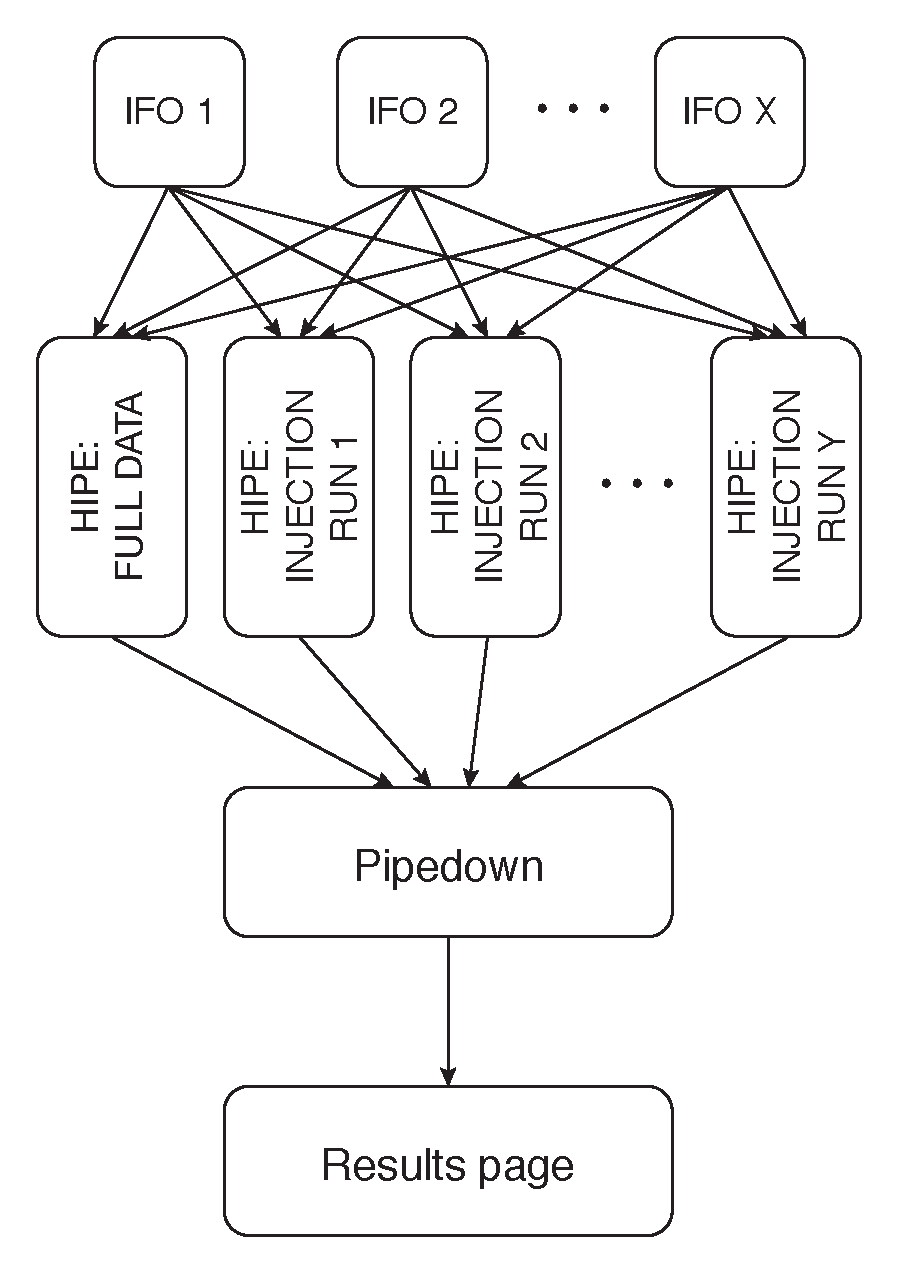
\includegraphics[width=2.5in]{figures/ihopeOverview.pdf}
\caption{
An overview of the \ihope~pipeline. The HIPE and Pipedown nodes are themselves
workflows, and are detailed in sections \ref{sec:HipeDetail} and
\ref{sec:PipedownDetail}, respectively. 
}
\label{fig:ihopeOverview}
\end{figure}

\section{Pipeline Requirements}
\label{sec:PipelineRequirements}

Here we briefly review the key requirements of a pipeline used to search for
\ac{GW}s. Our goal is to search for \ac{GW}s from coalescing binaries in a
range of masses. Since gravitational waves couple very weakly to matter we must
be able to detect strains of $\sim10^{-21}$ in noise that has an RMS amplitude
of $\mathcal{O}(10^{-22})$ at $100\,$Hz. Our target sensitivity is to detect
signals with a \ac{SNR} of $8$ in each detector.

When averaged over time the detectors' have a colored Gaussian noise
distrubtion; as shown in Chapter \ref{ch:pipeline_principles}, the optimal tool
to search for signals is therefore a matched filter \cite{Brown}. Match
filtering requires knowing the morphology of the waveform. Binaries with total
masses (\mtotal) less than $25\Msun$ emit most of their power in the \ac{LIGO}
and Virgo bands during their {\it inspiral} phases.  This means that the
waveform from these systems can be well modelled by the post-Newtonian
approximation. Thus, to cover the desired range,
we can fill a bank of templates using the methods described in section
\ref{sec:multiple_templates} of Chapter \ref{ch:pipeline_principles}.

Environmental and instrumental factors can cause non-Gaussian transient noise
(\emph{glitches}) in the data. To deal with this our pipeline must be able to
distinguish between triggers resulting from glitches and triggers resulting
from gravitational waves. Since the morhpologies of signals is known, and since
 the signals have a number of cycles in the frequency range (\emph{band}) we
are sensitive to, the $\chi^2$ test discussed in section \ref{sec:chisq} is a
powerful tool for discrimination \cite{Allen:2004}. Demanding that triggers be
coincident in multiple detectors using the e-thinca ellipsoids discussed in
section \ref{sec:coincidence_test} will also filter out spurious triggers,
since we do not expect environmental correlations across great distances
\cite{Robinson:2008}. After all filtering and tests have been applied, the
statistical significance of a set of triggers has to be evaluated to determine
the probability that a gravitational wave exists in the data. We can do this by
calculating the triggers' \emph{false alarm rates} (FARs) using the time-slide
method discussed in Chapter \ref{ch:far}. Since they only consist of noise
triggers (assuming equation \ref{eqn:valid_slide_condition} holds), the
coincident triggers resulting from time-slides are reffered to as
\emph{background}, to distinguish them from coincident triggers in which no
offset has been applied between detectors, or \emph{foreground}.

Even though we apply $\chi^2$ and coincidence tests, environmental factors can
cause periods of elevated glitch rate in the detectors. If these periods are
analyzed with periods of relatively clean data, they will pollute the
background estimation, thereby decreasing statistical confidence in candidates.
We therefore seek to remove such periods from the analysis. This is
accomplished using \emph{vetoes} \cite{Slutsky:2010ff, Christensen:2010}. A
veto is a half-open time-interval, or \emph{segment} in which all the triggers
are discarded. Vetoed time is not counted in the analyzed, or \emph{live}, time
when false alarm rates are calculated.

We define veto times by using \emph{\ac{DQ} flags}. The detectors are equipped
with environmental and instrumental monitors that are auxillary to the \ac{GW}
channel. If these channels detect periods of heightened activity in the
environment, such as elevated seismic noise, an automated monitor will mark the
period of time with a \ac{DQ} flag \cite{glitchmon}. Additional \ac{DQ} flags
can be added by hand; e.g., if a truck drives onto the site while \ac{GW} data
is being recorded, a person in the control room may add a flag for that period
of time.  The periods of time that these various flags are on are stored in a
\emph{segment database}, which is a central database that contains lists of
segments detailing the times that the detectors were in various states
\cite{BPP:segdb}. If a \ac{DQ} flag can be found to be strongly
correlated with elevated glitch rates in the \ac{GW} channel, and if it is
found that the flag is \emph{safe} --- i.e., it will not be triggered by a
\ac{GW} wave\footnote{This can be checked using hardware and software
injections.} --- then it is used as a veto. 

Vetoes are categorized according to how well we can couple them to known
environmental sources \cite{Slutsky:2010ff, Christensen:2010}. Table
\ref{tab:veto_cats} lists the various categories and their defining
characteristics. These categories are applied cumulatively. We refer to
category 1 vetoes as \emph{CAT1}. Category 1 and 2 vetoes are reffered to as
\emph{CAT2}; category 3 vetoes are refferred to as \emph{CAT3}. For \ac{CBC}
searches, we do not analyze anything prior to category 1; i.e., all matched
filtering is carried out after category 1 vetoes are applied. CAT2 and CAT3
vetoes are applied when second stage coincidence is carried out (see section
\ref{sec:second_thinca}, below). We quote false alarm rates and base upper
limits on data in which category 1-3 vetoes have been applied. We additionally
check the data after category 1 and 2 vetoes have been applied for any loud
triggers that may have been removed by category 3 vetoes. We do not use
category 4 for the analysis.  However, we do use category 4 vetoes in follow-up
studies of loud candidates to provide insight into the cause of triggers.
Hardware injections are left in the data after category 1 and 2, and are
removed as a special veto prior to category 3 vetoes being applied.

The use of vetoes is key to our ability to detect gravitational waves. Without
them, we could not detect signals at a \ac{SNR} of $8$ in each detector (see
Chapter \ref{ch:ligo_south_study}). To determe what \ac{DQ} flags are most
effective at removing triggers caused by environmental factors we perform
\emph{glitch studies}. This allows us to \emph{tune} vetoes such that we
maximize the probability of detecting a signal.

In addition to vetoes, each of the analysis methods described above have
various parameters that can be tuned. This includes the number of $\chi^2$ bins
to use \cite{Brown}, the $\chi^2$ threshold to apply \cite{Keppel:thesis}, the
duration of the $r^2$ veto \cite{Rodriguez:2007}, how finely to grid the
parameter space and what coordinates to use \cite{Owen:1998dk, Tanaka:2000,
BBCCS:2006, hexabank}, what \ac{pN} order to use to generate templates
\cite{Collaboration:2009tt, Abbott:2009qj, Collaboration:S6CBClowmass}, the
size of the e-thinca parameter \cite{Robinson:2008, Keppel:thesis}, the number
and placement of the chirp-mass bins for calculating \acp{FAR}
\cite{Keppel:thesis}, and many other paramters not discussed here. Like vetoes,
we wish to tune these parameters such that we maximize the probability of
detecting a signal. However, we must do this in a {\it blind} fashion. That is,
we must be able to tune parameters without knowledge of what is in the data,
else the results will sway in favor of the analysts' bias.

To satisfy these conflicting requirements, we have designated a subset of data
as \emph{playground}. Playground is defined as data that occurs during the
first $600$ seconds of every $6370$ seconds, starting from February 14, 2003 at
16:00:00 UTC (GPS time $729273613$). It therefore consists of $\sim10\%$ of the
full data. The results of tuning studies are evaluated by considering the
results of analyzing playground data. In addition to playground data, we permit
ourselves to look at the most significant (\emph{loudest}) coincidence triggers
from slide data when ranked by \ac{FAR}. If an auxillary environmental or
instrumental channel can be correlated with a loudest slide trigger, we can
veto it. (For more on these \emph{loudest slide studies} see chapter
\ref{ch:s6_results}.) Only after all of the vetoes and parameters have been
tuned do we look at, or \emph{un-blind}, the full data results to see if a
\ac{GW} candidate exists.\footnote{Full data results include data from
playground time. Although playground is included in the final unblinded
results, we exculde it for computing upper-limits \cite{Collaboration:2009tt,
Abbott:2009qj, Collaboration:S6CBClowmass}.} 

Finally, the pipeline must be able to evaluate its sensitivity and efficiency
to sources in the universe. Doing so allows tuning studies to be carried out
prior to doing the full analysis, and for the astrophysical rate of \ac{CBC}s
to be bounded after the analysis has completed. This can be done by performing
\emph{injections} of signals with known parameters into the detectors. Both
\emph{hardware} and \emph{software} injections may be performed. Hardware
injections involve actuating the mirrors to physically simulate a passing
gravitational wave. This is the most robust test as it checks the ability of
the detectors' response loop to measure \ac{GW} strains and the ability of the
pipeline to detect them. However, hardware injections prevent real \ac{GW}s
from being detected while they are occurring, limiting the number that can be
preformed.  Software injections involve adding a gravitational wave signal to
the data stream on disk just prior to analyzing it. While this method does not
test the hardware control systems, it has the advantage that it can be
performed many times in parallel, without corrupting the original data. Thus,
our pipeline must be able to perform software injections, and have a method for
associating triggers with the injections that went into the data.

In summary, a pipeline used to search for gravitational waves from \ac{CBC}s must:
\begin{itemize}
\item{construct a bank of templates with which to filter \cite{Owen:1998dk, Tanaka:2000, BBCCS:2006, hexabank};}
\item{identify \emph{triggers} by filtering templates through the detector data \cite{Brown};}
\item{distinguish noise triggers from gravitational wave triggers \cite{Allen:2004};}
\item{veto periods with elevated glitch rate due to environmental factors \cite{Slutsky:2010ff, Christensen:2010}}
\item{quantify statistical significance of triggers and rank them in a blind manner;}
\item{evaluate the sensitivity and efficiency of the search to \ac{CBC}s in the universe \cite{Collaboration:2009tt, Abbott:2009qj, Collaboration:S6CBClowmass}.}
\end{itemize}
In the following sections we will see how \ihope~meets these requirements.

\begin{table}
\label{tab:veto_cats}
\center
\begin{tabular}{c | p{5cm} | p{8cm}}
Category    &    Description    &   Procedure    \\
\hline
    1       &    Data seriously compromised or missing.    &    Data never analyzed. \\
\hline
    2       &    Instrumental problems with known coupling to h(t).    &    Vetoed triggers discarded after second coincidence. Surviving triggers checked for candidates, but not used for upper limits. \\
\hline
    3       &    Instrumental problems likely, casting doubt on triggers found during these times.    &    Vetoed triggers discarded after second coincidence. False alarm rates of surviving triggers are used in publications; upper limits are calculated using these vetoes.  \\
\hline
    4       &    Positive, but weak, correlations with false alarms. Large dead times.    &     Not used in the analysis, but used as a guide in detailed followups of loud triggers. \\
\end{tabular}

\caption{The various veto categories used by the CBC group. Vetoes are applied cumulatively; statistical significance of candidates and upper limits are calculated after category 1, 2, and 3 vetoes are applied.}
\end{table}

\section{\ihope~at Runtime}
\label{sec:ihopeRuntime}

The \ihope~pipeline is created by running \texttt{lalapps\_ihope}. This sets up
the workflow by doing the following at run time:

\begin{itemize}
\item{set-up the directory structure to save all data to;}
\item{copy all needed programs from their installed location to a local directory;}
\item{retrieve analysis start and stop times;}
\item{download a {\it veto-definer file} and find the start and stop times of all veto segments;}
\item{run \texttt{lalapps\_inspiral\_hipe} multiple times;}
\item{run \texttt{lalapps\_cbc\_pipedown};}
\item{create a cache file of the names and locations of all files that will be created;}
\item{write a DAG that can be used to start and run the worflow.}
\end{itemize}

These steps require the start and stop time (in GPS seconds) of the period to
be analyzed --- which we shall refer to as the \emph{analysis
period}\footnote{We typically analyze periods that are on order of a week to a
month. For analysis periods used in \ac{S5} and \ac{S6} see chapters
\ref{ch:s5_results} and \ref{s6:results}, respectively.} --- as well as a
\emph{configuration file}. The configuration file is a text file containing all
the information needed to setup and run the analysis. This includes: the names
and locations of all the executables that will be run; variable arguments that
these programs will need; the name and number of interferometers to analyze;
the version of data files to retrieve and what channels to analyze; how many
and what type of software injection runs to do; any other information needed by
the \ac{DAG}s to run. The configuration file provides a convenient way to
manipulate the pipeline. Changing tuning parameters is largely accomplished by
editing this file. Likewise, the difference between running a {\it low-mass}
search ($2 < \mtotal/\Msun < 25$) and a {\it high-mass} search ($25 <
\mtotal/\Msun < 100$) is determined entirely by the configuration file.

A directory named by the gps start/stop times of the analysis period is created
at runtime. All work is done in this directory. In it, a \texttt{segments},
\texttt{executables}, \texttt{datafind}, \texttt{full\_data}, and
\texttt{pipedown} directory are created, along with a directory for each
injection run that will be carried out. With the exception of the
\texttt{executables} and \texttt{segments} directory, each of the sub
directories store a sub-\ac{DAG} that will be run during the analysis (and will
be explained below). The master \ac{DAG} is saved in the gps-times direcotory
along with a master cache file of all the files that will be created. All
programs that will be run are copied to the \texttt{executables} directory.

\subsection{Science and Veto Segments Retrieval}
\label{sec:science_segs_and_vetoes}

During a Science run the \ac{LIGO} and Virgo detectors can be in one of several
different states at any given time, which we categorize into five different
operating modes. We are only interested in analyzing times in which the
detectors are in {\it Science} mode. This means they are
``locked,"\footnote{Recall from Chapter \ref{ch:theory} that the interferometer
light must be resonant in the Fabry-Perot cavities for the interferometer to
operate. We refer to this as the interferometer being ``in lock."} no other
experimental work is being done on them, and their state has been verified by a
human. The interferometers can come out of Science mode many times across an
analysis period; thus \ihope~must retrieve the start and stop times of Science
segments that occurred in the analysis period. \verb|Ihope| does this by
running \texttt{ligolw\_segment\_query} \cite{BPP:segdb} at run time. This program queries the
segment database (described above) to retrieve the list of Science times during
the desired analysis period.  These results are saved to files in the
\texttt{segments} directory. These files do not contain strain data; they only
list the times that data can be retrieved. The results are later used to
retrieve files containing strain data.

The Science segments, as well as most of the results of each step in the
pipeline, are saved in \emph{XML} files. An XML file stores data in a
hierarchical structure of ``elements," where each element may contain other
elements \cite{tech:Williams:2005}. In our case, the elements of the document
are data tables; in turn, the data tables have columns, which are the elements
of the table. The XML files used by \ihope~conform to the \verb|LIGO_LW| data
format, which specifies how tables and columns are named, and how they are
stored to XML files. For more details on XML and the \verb|LIGO_LW| format see
\cite{tech:Williams:2005}.

As discussed in section \ref{sec:PipelineRequirements}, all of the \ac{DQ}
flags that may be used for vetoes are stored in the segment database
\cite{BPP:segdb}. What flags to use for vetoes, at what category, and for how
long, are stored in a \emph{veto-definer file}. This XML file contains a
\texttt{veto\_definer} table that lists each flag that should be used, what
category the flag should be used at, the dates the flag is valid, and any
padding (in seconds) to add to the flag. The table is veto-definer file is
created by analysts who carry out studies to determine what \ac{DQ} flags to
use for a specific search. These studies draw on a number of different
resources, including: data-monitoring tools that run at the observatories, an
online log, or \emph{e-log} that scientists use document events and studies
carried out at the observatories,\footnote{See section \ref{sec:printlc-minifups} for
more details on the e-log.} as well as results \ihope~produces from playground
data and injection studies. Entries are added to this table by hand after
extensive data-quality investigations and safety checks.\footnote{For more
details on how these studies were carried out for the low-mass \ac{CBC} search
in \ac{S6}, see chapter \ref{ch:s6_results}.} Vetoes are fine tuned for
specific searches and Science runs; each searches' set is saved in a different
veto-definer file in a central repository. What veto definer file to use is
specified in the \ihope~ configuration file. At run-time, \ihope~downloads the
desired file to the \texttt{segments} directory. It then runs
\texttt{ligolw\_segments\_from\_cats} \cite{BPP:segdb} to query the segment
database for flags specified in the veto-definer file. The vetoed segments for
all of the instruments are added together and saved in XML files in the
\texttt{segments} directory.


\subsection{HIPE}
\label{sec:hipe_overview}

Once the analyzable Science segments and the veto segments that will be applied
are obtained, \ihope~runs \texttt{lalapps\_inspiral\_hipe}. This sets up the
\hipe~\acp{DAG}, which are the pipelines that carry out the search. Figure
\ref{fig:HIPEDiagram} shows a \hipe~\ac{DAG} for a single $2048\rm{s}$ block of
time. As can be seen in the diagram, \hipe~is a \emph{two-stage} pipeline. Data
is matched-filtered \cite{Brown}, coincidence tests \cite{Robinson:2004} are applied, then the process is
repeated. The reason for using two-stages is the $\chi^2$ test is
computationally expensive \cite{Allen:2005fk}. To reduce the number of triggers for which we need
to compute $\chi^2$, an initial coincidence test is applied to single-detector
triggers for which only \ac{SNR} is calculated.\footnote{Using two stages
complicates the pipeline, however, and makes it difficult to trace an event's
progression through the various steps. It also hampers efforts to estimate
\acp{FAR} from single-detector triggers. For this reason, a single-stage
pipeline is being developed which takes advantage of advances in computational
power. See Chapter \ref{ch:future_developments} for more details.} Recall from
Chapter \ref{ch:pipeline_principles} that a coincidence test reduces the number
of triggers in the detectors since noise sources are uncorrelated between the
sites.\footnote{There are correlated noise sources between the two Hanford
interferometers, H1 and H2, so this test is less effective for those two
interferometers.} After applying this \emph{first coincidence} test, we
calculate $\chi^2$ for the surviving triggers and apply the $\chi^2$ threshold
and $r^2$ veto. We then perform a \emph{second coincidence} test to check for
coincidence among triggers that survived the $\chi^2$ cuts \cite{Allen:2005fk}.

\hipe~can be run either with or without software injections. If injections are
desired, \texttt{lalapps\_inspinj} is run to create a list of injections to
perform,\footnote{See section \ref{sec:inspinj} for details on how this is
done.} which are created and inserted into the data just prior to match
filtering by \texttt{lalapps\_inspiral} \cite{brown-2005-22} when the \ac{DAG}
is run. At run-time \ihope~runs \hipe~several times: once for each desired
injection \ac{DAG}\footnote{The number of injection runs to carry out and the
types of injections to perform in those runs are specified in the configuration
file.  See section \ref{sec:inspinj} for more details.} and once each for
\emph{zero-lag} and \emph{time-slid} data. Zero-lag data is data for which the
coincidence test is applied \emph{without} adding a time offset to each
detector. This is the data that could potentially contain coincident triggers
from \acp{GW}.  ``Time-slid" data is data for which the coincidence test is
applied after adding a time offset to each detector. Since the data is slid
such that the offset is larger than the light-travel time between the
detectors, time-slid contains ``accidental" coincidences, i.e., we do not
expect single-detector triggers from a single \ac{GW} to be coincident with
each other in time-slid data. This is the data we use for our \emph{background}
when calculating false alarm rates. (For details, see Chapter \ref{far}.) Each
of these \hipe~\acp{DAG} are distinguished from each other by a
\emph{user-tag}. Zero-lag data is labelled \verb|FULL_DATA|, while time-slid
data is labelled \verb|FULL_DATA_SLIDE|. The user tag to use for each injection
\ac{DAG} is set in the configuration file by the analyst.

A description of what each program does when the \hipe~\acp{DAG} are launched
are discussed in section \ref{sec:HIPEdetail}.

\begin{figure}[p]
\begin{center}
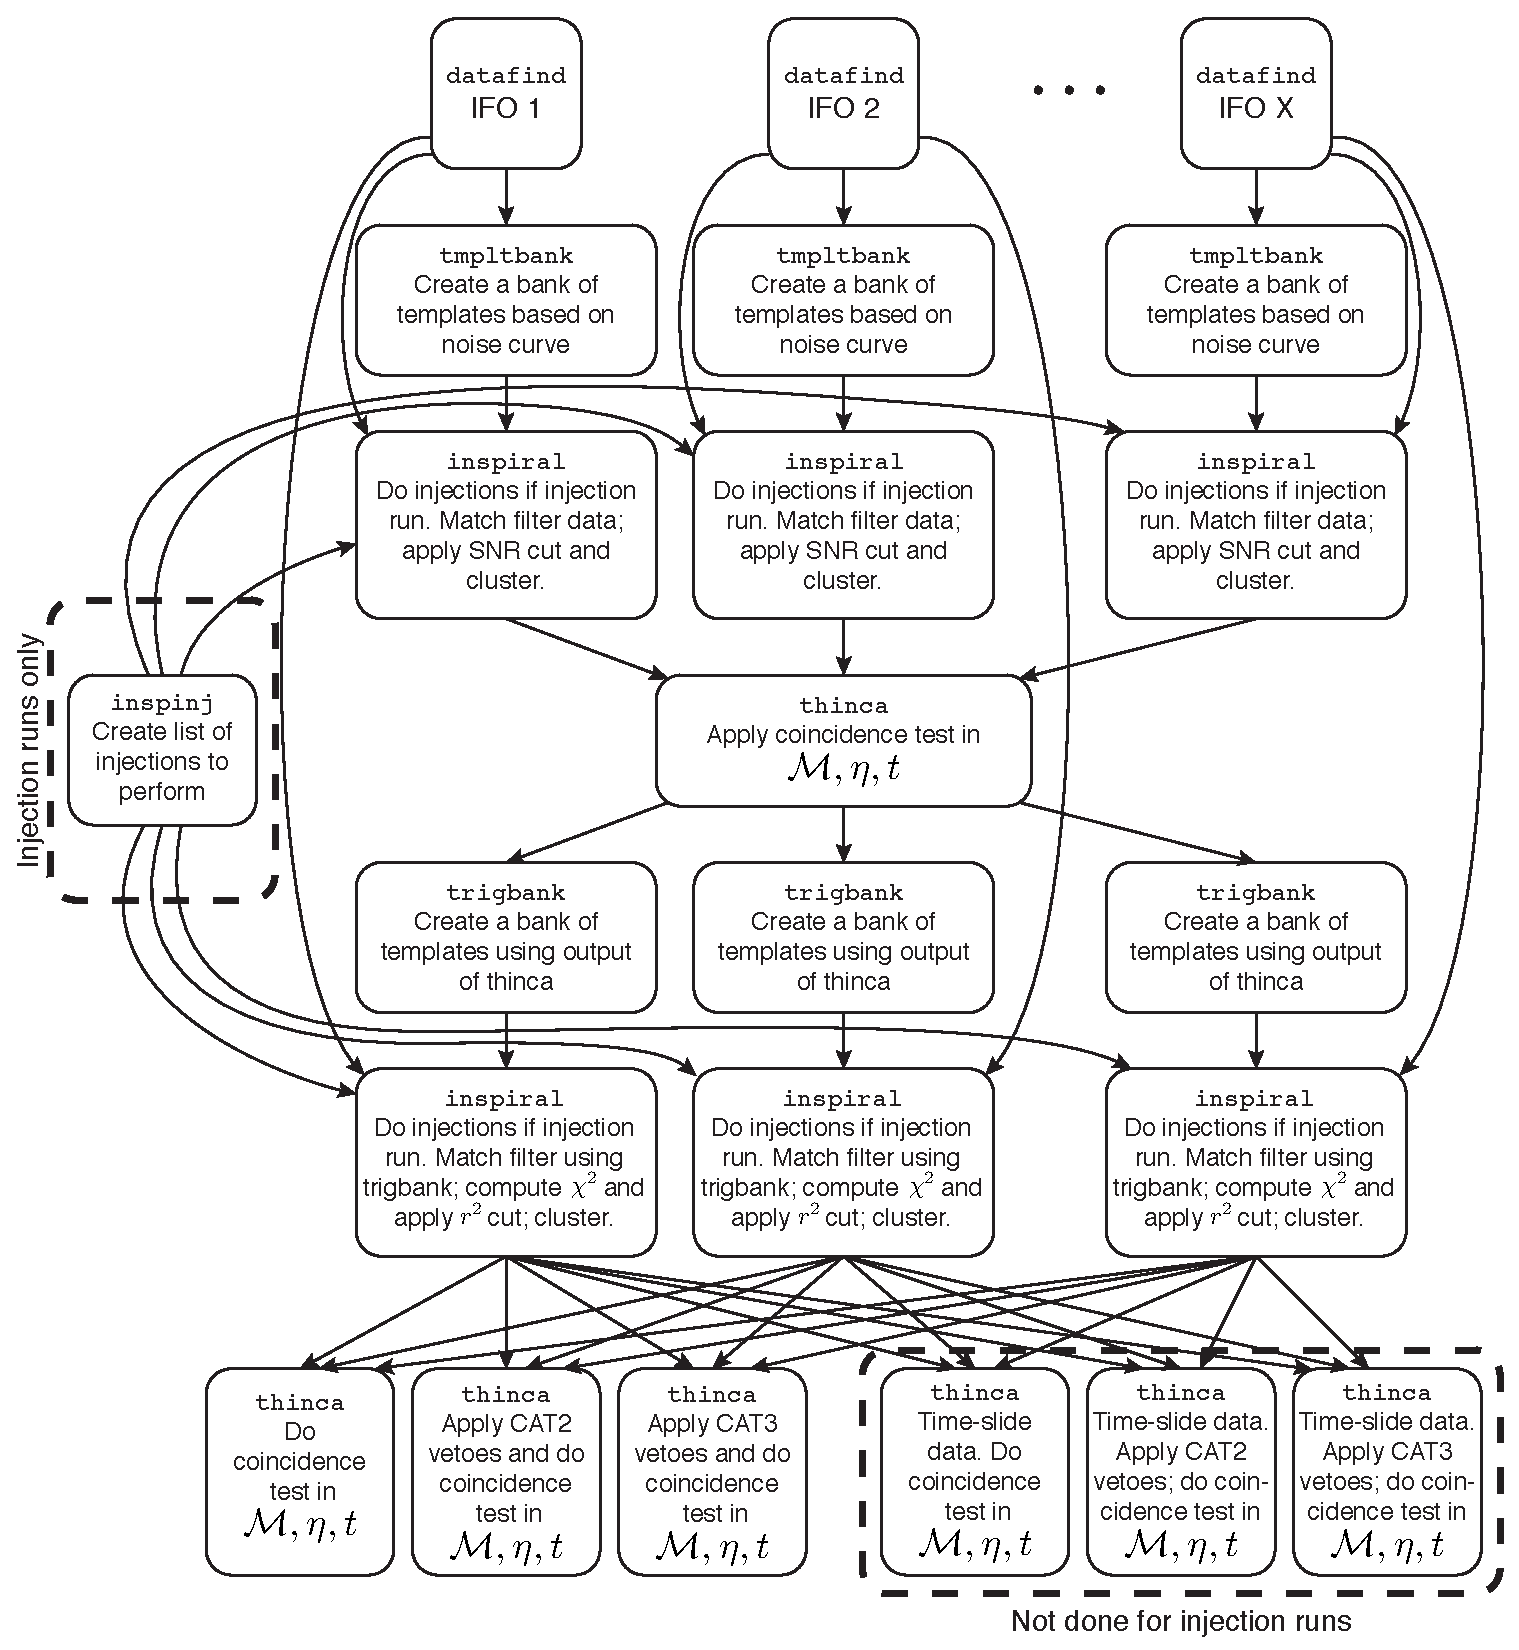
\includegraphics[width=6in]{figures/HIPEDiagram.pdf}
\end{center}
\caption{
The \hipe pipeline. This is run once for full-data and once for
each injection run. For injection runs, \texttt{lalapps\_inspinj} is run to
generate a list of injections to create, and time slides are not done.
}
\label{fig:HIPEDiagram}
\end{figure}

\subsection{Pipedown}
\label{sec:pipedown_overview}

After all the instances of \texttt{lalapps\_inspiral\_hipe} have run, \ihope~
runs \texttt{lalapps\_cbc\_pipedown} which sets up the Pipedown \ac{DAG}.
Pipedown takes the results of all the different HIPE \acp{DAG}, combines them into
SQLite databases, computes and ranks triggers by \ac{FAR}, and creates plots
and tables of the results. Figure \ref{fig:PipedownDiagram} details the steps
Pipedown takes to carry out these goals. Shown are the steps taken for a single
veto-category; this diagram is repated for each veto-category (by Pipedown, not
by \ihope). In-depth details of Pipedown are discussed in Section
\ref{sec:PipedownDetail}.

\begin{figure}[p]
\begin{center}
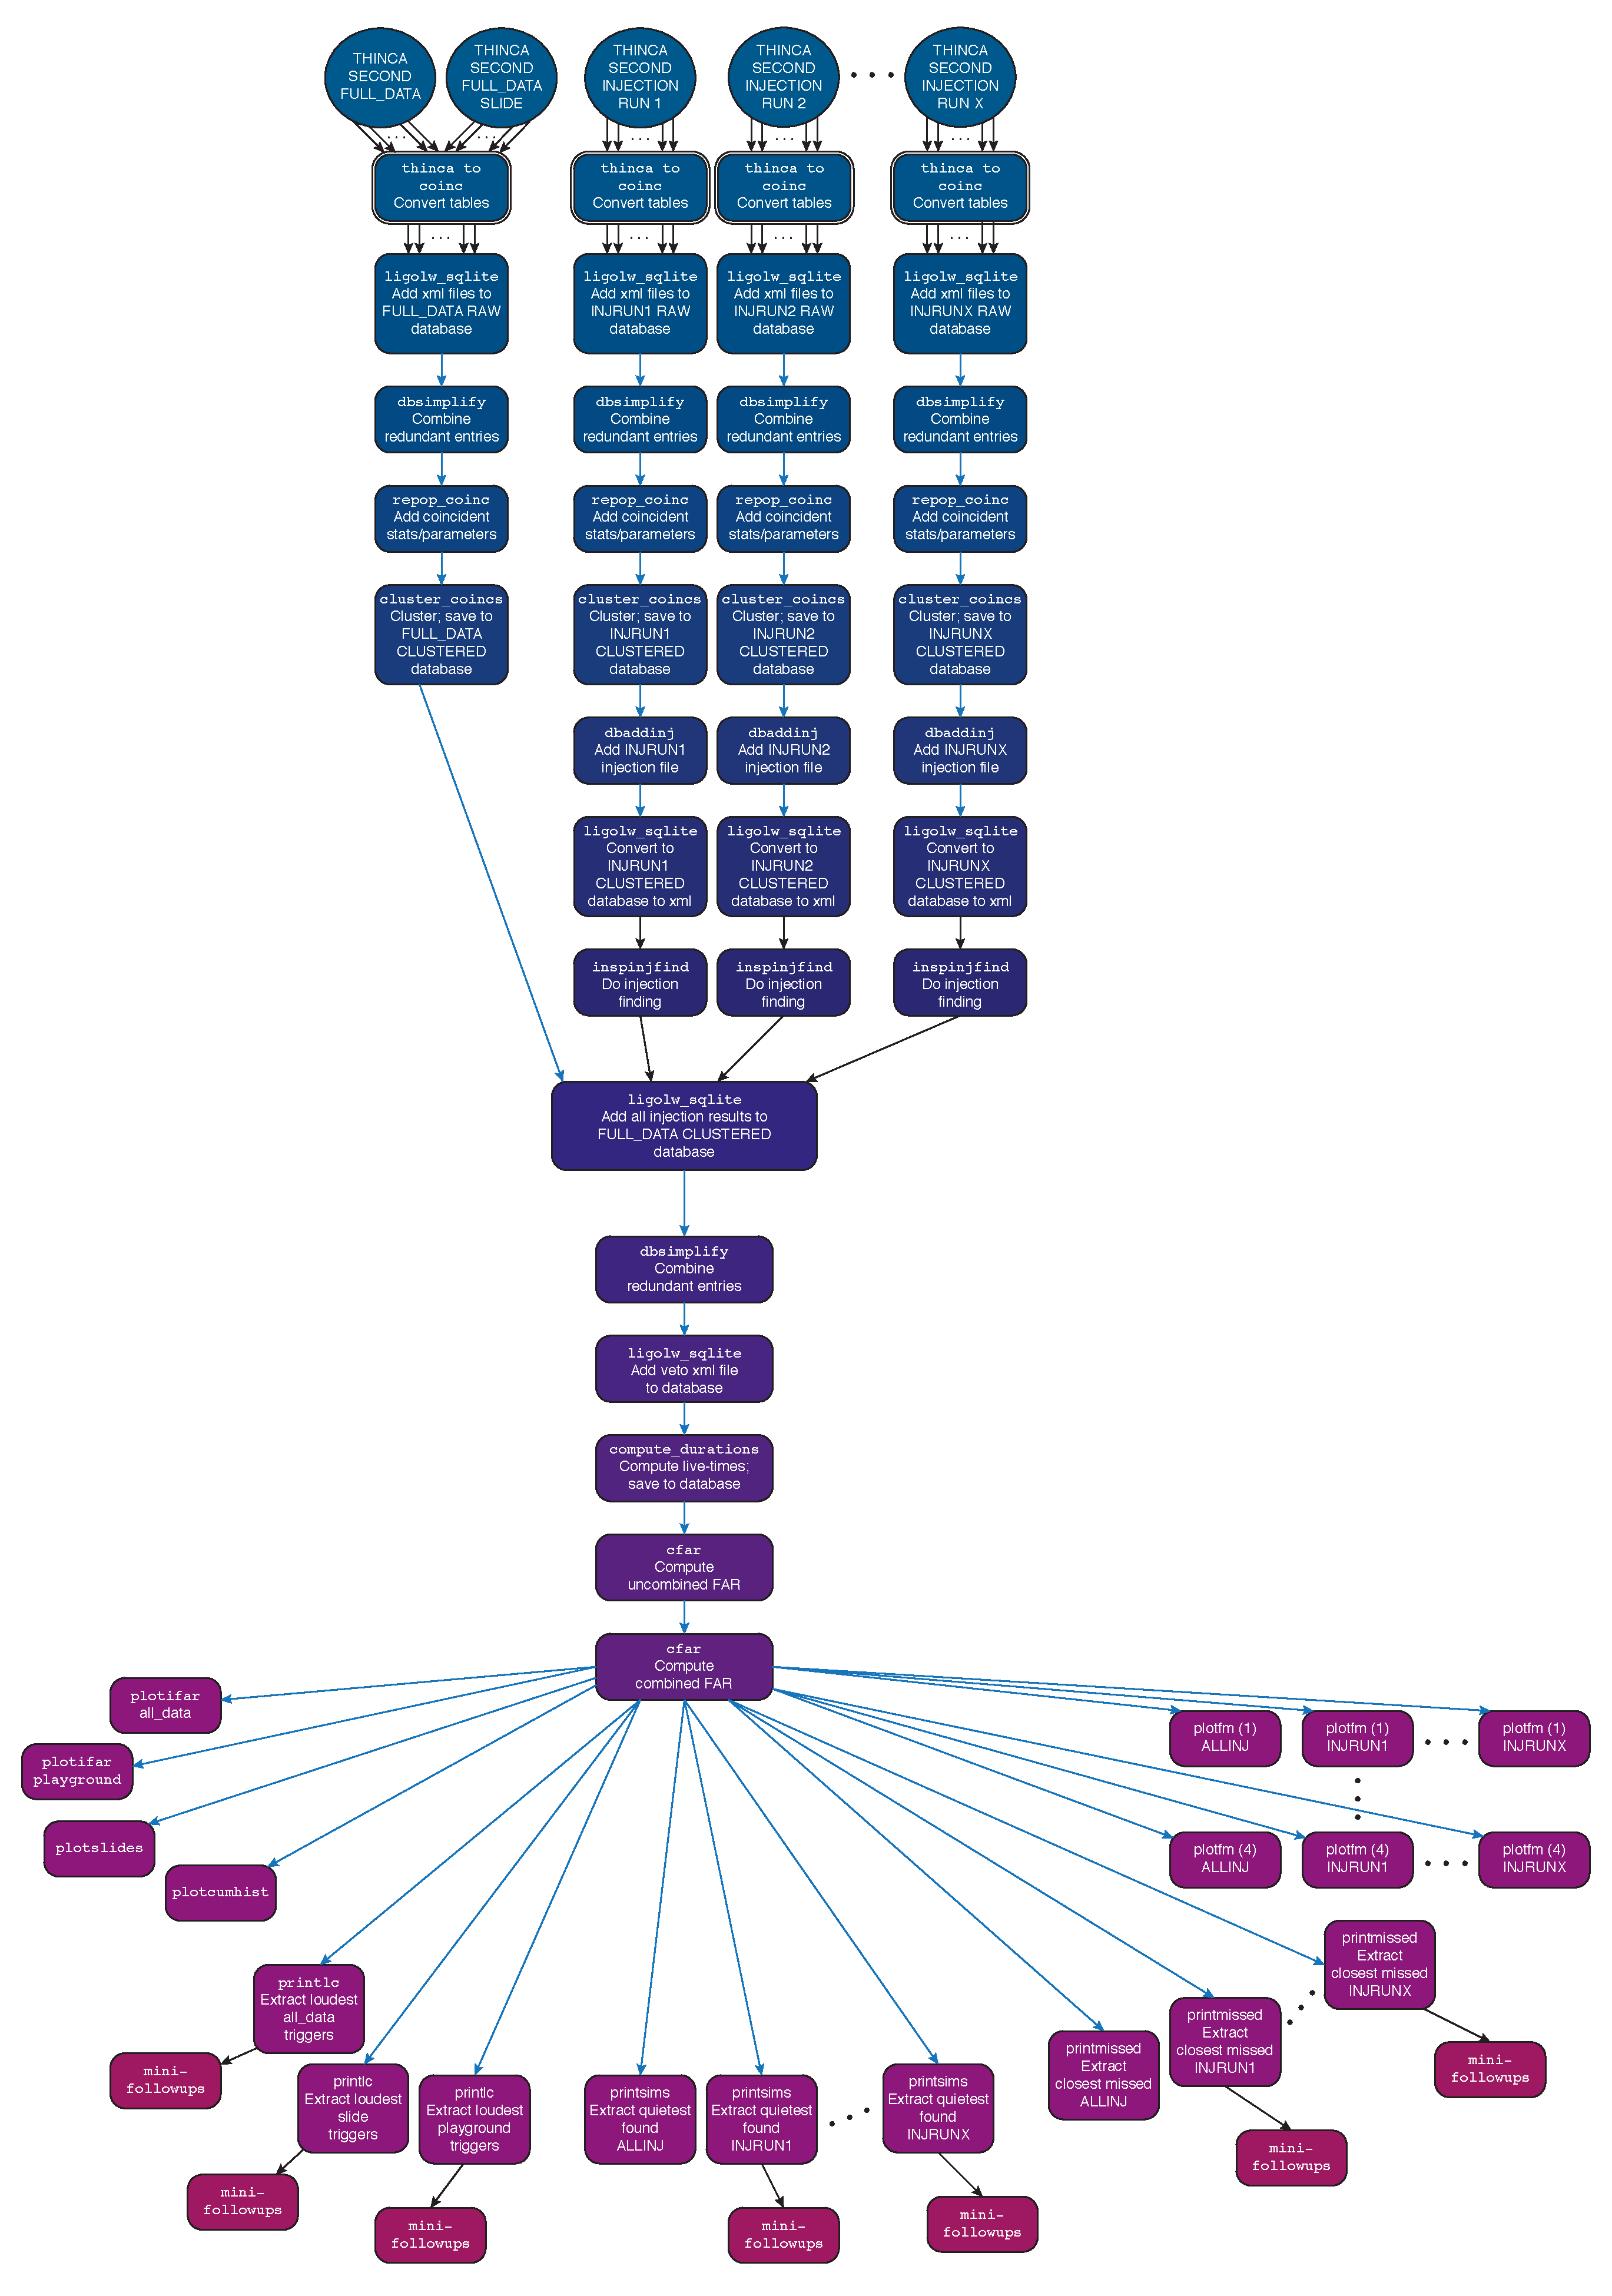
\includegraphics[width=6in]{figures/PipedownDiagram.pdf}
\end{center}
\caption{
The Pipedown pipeline for a single veto category. Each block represents a
single node. Double bordered blocks represent multiple nodes. Circles represent
batches of files. Black arrows represent XML files; blue arrows, SQLite
databases. Each arrow represents a single file.
}
\label{fig:PipedownDiagram}
\end{figure}

\subsection{DAX}
\label{sec:DAX}

After pipedown has completed, \ihope~writes a \emph{DAX} that can be used to
launch the pipeline. A DAX is an abstract workflow in which elements such as
file locations are variables. The DAX is turned into a \ac{DAG} by the Pegasus
Workflow Management Service \cite{dax:Pegasus}. The \hipe~\acp{DAG} are then
distributed across a compute cluster; after they finsish, the Pipedown \ac{DAG}
is launched.

\subsection{The Pipeline in Detail}

Now that we have established an overview of \ihope, we will step through it in
detail, using a toy analysis period of $10\,240$s as an example. In this
analysis we will use three interferometers: the 4-kilometer Hanford detector
(H1), the 4-kilometer Livingston detector (L1), and the 3-kilometer Virgo
detector (V1), and we will add one injection run, which we label
\texttt{BNSINJ}. In section \ref{sec:HIPEdetail} we step through each of the
programs that \hipe~launches to carry out the analysis. Next, in section
\ref{sec:Pipedown} we detail the programs launched by Pipedown in order to
combine results from the \hipe~\acp{DAG}.

The programs run in the \hipe~\ac{DAG} have been presented in prior
publications; c.f. \cite{brown-2005-22, Allen:2005fk, Robinson:2008,
Keppel:thesis}. Here, we provide a review of how each of these programs are run
in \ihope. Pipedown is a new addition to the \ihope~pipeline, and is presented
here for the first time. The routines the Pipedown programs carry out to
compute false alarm rates are based on earlier programs described in
\cite{Keppel:thesis}, however.

\section{HIPE in Detail}
\label{sec:HIPEdetail}

Figure \ref{fig:science-selected_segs} shows the segments that are available to
analyze during our toy analysis period. The \emph{selected segments} are
Science segments minus CAT1 veto segments; they are what \ihope~passes to
\hipe~to analyze. Figure \ref{fig:segment_plot_full} shows all of the XML files
that the \verb|FULL_DATA| \hipe~\ac{DAG} creates in our toy analysis. We will
use this figure and Figure \ref{fig:HIPEDiagram} as guides as we step through
each stage of \hipe. 

\subsection{Data Find}
\label{sec:data_find}

As can be seen in Figure \ref{fig:HIPEDiagram}, the first step in \hipe is to
run \texttt{ligo\_data\_find}. Data from all of the interferometers are stored
in \emph{frame files} in central locations at every computer cluster. Frame
files can contain multiple channels recorded from the interferometers. For
analysis purposes, we are only interested in files containing the strain data
channel, which is called \texttt{LDAS-STRAIN} in the \ac{LIGO} detectors and
\texttt{h\_16384Hz} in Virgo. \texttt{ligo\_data\_find} locates where the frame
files covering the selected segments are in the file system on the cluster. It
then creates a cache files listing the location of each these files in the
\texttt{datafind} directory. These cache files are passed to
\texttt{lalapps\_tmpltbank} and \texttt{lalapps\_inspiral}, which use them to
locate and open the frame files for analysis.

\subsection{From Continuous to Discrete Data}
\label{sec:cont_to_discrete}

All of the equations we used Chapter \ref{ch:pipeline_principles} involving
Fourier Transforms and the inner product have assumed continuous time- and
frequency-domain data series.  Likewise, the integrals over frequency space
were from $-\infty$ to $+\infty$. In practice, of course, the data is
discretely sampled and is neither continuous nor infinite in extent. Both the
\ac{LIGO} and Virgo strain data are sampled at $16384\,\mathrm{Hz}$. Since even
the lowest mass templates (i.e., waveforms with the highest frequency
components) used in current \ac{CBC} searches terminate at frequencies
$\sim1.5\,$kHz, this sampling rate is much higher than is needed for our
purposes. To ease computational requirements the time series is therefore
downsampled to $4096\,\mathrm{Hz}$ prior to analysis \cite{brown-2005-22}. This
sampling rate sets the Nyquist frequency, $f_{\mathrm{Nyquist}}$, at
$2048\,\mathrm{Hz}$. To prevent aliasing, a low-pass time-domain digital filter
with a cutoff at $f_{\mathrm{Nyquist}}$ is implemented to pre-condition the
data \cite{brown-2005-22}. On the low-frequency end, seismic noise dominates
the interferometers' power spectrum.  We therefore also impose a high-pass
digital filter in the time domain. The cutoff frequency of the high-pass
filter, $f_c$, is set to be a several Hz lower than a low-frequency cutoff,
$f_0$, that is determined by the characteristics of each detector's power
spectrum. These values are set in the configuration file.\footnote{In both
\ac{S5} and \ac{S6}, $f_0$ was set to $40\,$Hz for the \ac{LIGO}
interferometers due to the rising seismic noise at that frequency (see Figure
\ref{fig:init_AdvASD}). For Virgo's first science run, $f_0$ was set to
$60\,$Hz \cite{S5LowMassLV}; for \ac{VSR2} and 3 this was reduced to $50\,$Hz
(see Chapter \ref{ch:s6_results}). For all interferometers, $f_c$ was set to
$30\,$Hz~in~\ac{S6}.} Both the low- and high-pass filters will ring at the
start and end of a time series, corrupting the data. Thus we must remove the
first and last $t_{\mathrm{pad}}$ of data after applying the filters and prior
to analyzing. The duration of $t_{\mathrm{pad}}$ is also set in the
configuration file; for both \ac{S5} and \ac{S6} we used $8\,$s.

To Fourier Transform the data, we use the \ac{FFT} algorithm
\cite{Allen:2005fk}. The \ac{FFT} imposes two constraints on the data. First,
the number of points in the data series must be a power of two. Second, the
\ac{FFT} associates the last point of the data series with the first point;
i.e., it wraps the data around on a loop. This means that as a template is
filtered toward the end of the time series, any points extending beyond the end
of the series will be placed at the beginning, corrupting the data. Thus the
first $t_{\mathrm{chirp}}$ points of the \ac{SNR} time series are corrupted,
where $t_{\mathrm{chirp}}$ is the \emph{chirp length} of the template, and must
be thrown out \cite{Brown}.

The chirp length is defined as the length of time it takes for the binary to go
from $f_0$ to the frequency at which the binary passes \ac{ISCO},
$f_{\mathrm{isco}}$. As discussed in Chapter \ref{ch:theory}, the \ac{pN}
approximation breaks down at $f_{\mathrm{isco}}$; therefore we must terminate
all integrals at this point. Combining this with the limits of Nyquist and
seismic noise, all frequency domain integrals are limited to the region $f \in
[f_0, f_{\mathrm{max}})$ where $f_{\mathrm{max}} =
\min(f_{\mathrm{Nyquist}},~f_{\mathrm{isco}})$ \cite{ref:Brown}.

The \ac{PSD} is estimated using a variation of Welch's method \cite{Brown}.
This involves breaking a data segment up into several bins of equal duration.
Within each bin, the data is transformed to the frequency domain via the
\ac{FFT}. Thus the number of points in each bin must be a power of two, and the
bins must be overlapping to account for corruption at the beginning and end of
each segment. Since the data is discrete, this results in a discrete number of
frequency bins. The \emph{median} value within each frequency bin is then
chosen across all the data segments to construct $S_n(|f|)$. We use the medain
--- as opposed to the mean --- to buffer the \ac{PSD} from over-estimation in
the prescence of a signal or glitches \cite{Brown}.

The computation of $S_n(|f|)$ is also affected by the discontinuity between the
first and last point of the data time-series. Additionally, recall from Chapter
\ref{ch:pipeline_principles} that to match filter the data, we filter
$\widetilde{s}(f)$ with:
\begin{equation*}
\frac{\widetilde{h}^{*}(f)}{S_n(|f|)}
\end{equation*}
This is known as the \emph{kernel} of the filter. Since $S_n(|f|)$ is a part of
the kernel, the impulse response of the kernel is such that the entire data
series would be corrupted if a delta function existed in the data. To limit the
corruption due to the wrap-around and the ``ringing" of the kernel, we
\emph{truncate} the \ac{PSD} \cite{Brown}. This is done by estimating \ac{PSD}
using Welch's method, inverse transforming $\sqrt{S_n^{-1}(|f|)}$ to the time
domain, zeroing out the first and last $t_{\mathrm{invspectrunc}}$ seconds of
the time series, then transforming back to the frequency domain. This limits
the corruption due to the wraparound to the first and last
$t_{\mathrm{invspectrunc}}$ seconds of the time series. The truncation does
cause some smoothing out of high Q features, such as power-line harmonics;
however, since we search for relatively broad band signals this smoothing has
little effect on the search. The value of $t_{\mathrm{invspectrunc}}$ was set
to $8\,$s for both \ac{S5} and \ac{S6}.

For more details on how the \ac{PSD} is estimated and the matched filter is
implemented in \acp{CBC} searches, see \cite{Brown} and \cite{Allen:2005fk}.

\subsection{Data Segmentation}
\label{sec:data_segmentation}

\texttt{lalapps\_inspiral} is the program that constructs the \ac{SNR} time
series for templates laid out in a bank by the program
\texttt{lalapps\_tmpltbank} \cite{brown-2005-22}. The \ac{SNR} time series is
constructed according to equation \ref{eqn:snr_full_form} and the templates are
laid out using the metric defined in equation \ref{eqn:templateMetric}. Since
both of these equations involve the inner product defined in equation
\ref{eqn:eqn:inner_product2}, both programs must compute the \ac{PSD},
$S_n(|f|)$, as well as the Fourier Transform of the data,
$\widetilde{s}(f)$.\footnote{We do not Fourier Transform the templates as this
would be computationally expensive \cite{Brown}. Instead, we use the
\emph{stationay-phase approximation}, which is an analytical method that allows
us to express the templates in the frequency wave directly
\cite{WillWiseman:1996, Cutler:1994}. For a derivation, see \cite{Brown}.}

The wrap around of the \ac{FFT} and the Welch median \ac{PSD} estimation method
put limitations on how much data can be analyzed at once; they also require
data to be overlapped due to corruption at the start and end of segments. These
considerations require us to carefully segment the data for analysis. The
things we must consider are \cite{Brown}:
\begin{itemize}

\item{The low-pass and high-pass digital filters corrupt the first $8\,$s of an
analysis segment, or \emph{block}.}

\item{In order to estimate the \ac{PSD} using the Welch median method, we must
break the block up into several segments; data in each segment is transformed
via the \ac{FFT} independently.}

\item{The \ac{FFT} requires the number of points in each segment to be a power
of two.}

\item{The wrap around of the \ac{FFT} causes the first $t_{\mathrm{chirp}}$
seconds of each segment to be corrupted due to the template, and the first and
last $8\,$s of the segment to be corrupted due to the inverse \ac{PSD}.}

\item{Each segment must therefore overlap so as not to lose data from the
corrupted parts of the \ac{FFT}.}

\end{itemize}
In initial and enhanced \ac{LIGO} the low-frequency cutoff $f_0$ was set to
$40\,$Hz (see Figure \ref{fig:init_AdvASD}. In the low-mass \ac{CBC} search,
the longest template is therefore $\sim33\,$s in duration. The smallest power
of two larger than $33$ is $64$; thus the first $64\,$s of each segment must be
overlapped by a previous segment. The end of each segment only needs to be
overlapped by $8\,$s to account for the \ac{PSD} corruption. However, for
book-keeping simplicity, the last $64\,$s of each segment is also discarded.
Thus, all the segments must overlap each other by $128\,$s. Since the segments
must be a power of two, this means each segment must be $256\,$s in duration
\cite{Brown}.

In deciding upon the number of segments to use in the median \ac{PSD} estimate
we must consider a few factors. The more segments we have, the more accurate
the \ac{PSD} estimation will be. However, more segments also means that more
time will be grouped together. If the \ac{PSD} changes over this period, our
estimate will be off. Furthermore, the number of segments used sets a minimum
period of time that we must have continuous data. If a selected segment is
shorter than that period, we cannot analyze it. 

In inital and enhanced \ac{LIGO} we have chosen to use 15 overlapping segments
for each \ac{PSD} estimation. Since each segment is $256\,$s long, with
overlaps of $128\,$s, this means that each block must be $2048\,$s long. Add to
this the needed $8\,$s pad at the start and end of the block to account for the
corruption of the filters, and we find that we need a continous $2064\,$s of
data in order to do the analysis. If a selected segment is longer than
$2064\,$s, then it will be broken up into several blocks. Each block is
overlapped by $72\,$s to account for the time thrown out at the beginning/end
of the first/last segment in each block and the $8\,$s pad. If the selected
segment is not a multiple of $2048$ (as it most likely will not be), then the
last block in the segment is overlapped more so as to analyze the entire
period. The segments in this last block that overlap with non-corrupted time in
the previous block are simply not match filtered, although they are used for
the \ac{PSD} estimation of the last block.

The effects of this data segmentation on our toy analysis can be seen in Figure
\ref{fig:segment_plot_full}. The top three lines show the selected segments.
Each \texttt{TMPLTBANK} and \texttt{INSPIRAL} jobs corresponds to a single
chunk in a single detector. As can be seen, every chunk overlaps by $72\,s$,
except for the last one in each segment. Also note the first selected segment
in V1. As seen in Figure \ref{fig:science-selected_segs}, a CAT 1 veto broke
the V1 Science segment into two selected segments. Since the first selected
segment is only $\sim900\,$s long, it cannot be analyzed. This can be seen in
the \texttt{TMPLTBANK} and \texttt{INSPIRAL} lines: there are no V1 jobs
covering this period. This is part of the reason why CAT 1 vetoes are only used
for seriously compromised data. Overuse of CAT 1 vetoes could lead to large
amounts of unanalyzed time if they broke the data up into selected segments
that were shorter than $2064\,$s.

\subsection{Template Bank}
\label{sec:tmpltbank}

The first step in the \hipe~pipeline after \verb|data_find| is to create a
\emph{template bank}.\footnote{Recall from section \ref{sec:multiple_templates}
that a template bank is a collection --- or \emph{bank} --- of waveforms -- or
\emph{templates} --- that cover a parameter space. How they are laid out is
determined by computing a metric on the parameter space \cite{Owen:1995tm,
Owen:1998dk, Tanaka:2000, BBCCS:2006, hexabank}.} As stated above,
\texttt{lalapps\_tmpltbank} is the program that constructs the bank.
\hipe~creates one \texttt{tmpltbank} job for each detector and for each chunk.
Since the \ac{PSD} is re-estimated for each chunk the metric on the parameter
space (given in equation \ref{eqn:templateMetric}) will change from job-to-job,
resulting in a different template bank for each analysis block and for each
detector. However, the changes in the \ac{PSD} are usually small, and so the
bank stays roughly the same across an analysis period. In order to calculate
the \ac{PSD} \texttt{lalapps\_tmpltbank} reads in the frame cache, loads the
data, applies the low- and high-pass filters, downsamples to $4096\,$Hz, then
computes the \ac{PSD} using the Welch median method \cite{Allen:2005fk}.

Variables such as what \ac{pN} order to use to lay out templates, what space to
lay them out in, and what minimal match to use are command-line arguments to
\texttt{lalapps\_tmpltbank} and can therefore be set in the configuration file.
As stated in Chapter \ref{ch:pipeline_principles}, for \ac{S5} the bank was
laid out in $\tau_0$ and $\tau_3$ space using $2.0$ restircted \ac{pN}
templates to calculate the metric, such that the maximum loss in \ac{SNR} due
to the discreteness of the bank is $\sim3\%$ \cite{Collaboration:2009tt,
Abbott:2009qj, Collaboration:S6CBClowmass}. By \ac{S6}, it was possible to
generate restricted $3.5$\ac{pN} templates. However, the bank metric and best
coordinates to use to lay out templates is unknown at $3.5$\ac{pN} order. While
the \ac{pN} order of the templates should be the same as the \ac{pN} order used
to calculate the bank metric, it was found that using $3.5\,$\ac{pN} waveform
with a 2\ac{pN} metric did not significantly hurt the efficiency of the
pipeline to recover software injections. As a result, restricted $3.5\,$\ac{pN}
templates were used in \ac{S6} and they were laid out using the $2\,$\ac{pN}
metric.

Figure \ref{fig:template_bank} shows a typical template bank in both
$\tau_0,~\tau_3$ space and in $m_1,~m_2$ space for the low-mass \ac{CBC}
search.\footnote{Note that the maximum total mass in these plots extends to
$35\,\Msun$. This was reduced to $25\,\Msun$ for the last part of \ac{S6}. See
Chapter \ref{ch:s6_results} for details.} The parameters of each of these
templates are stored in a \texttt{sngl\_inspiral} table (the ``\texttt{sngl}"
stands for ``single"; see section \ref{sec:data_storage} for more details),
which is saved in an XML file. Also stored in the \texttt{sngl\_inspiral} table
are the metric components around each template. Each \texttt{tmpltbank} job
outputs one XML file, with naming convention: \begin{center}
\texttt{\{IFO\}-TMPLTBANK-\{GPS-START\}-\{DURATION\}.xml} \end{center} All of
the \texttt{tmpltbank} files created in our toy $10\,240\,$s analysis can be
seen in Figure \ref{fig:segment_plot_full}.

\begin{figure}[htbp]
\center
\subfigure[$\tau_3$ vs. $\tau_0$]{\label{fig:tmpltbank-tau0tau3}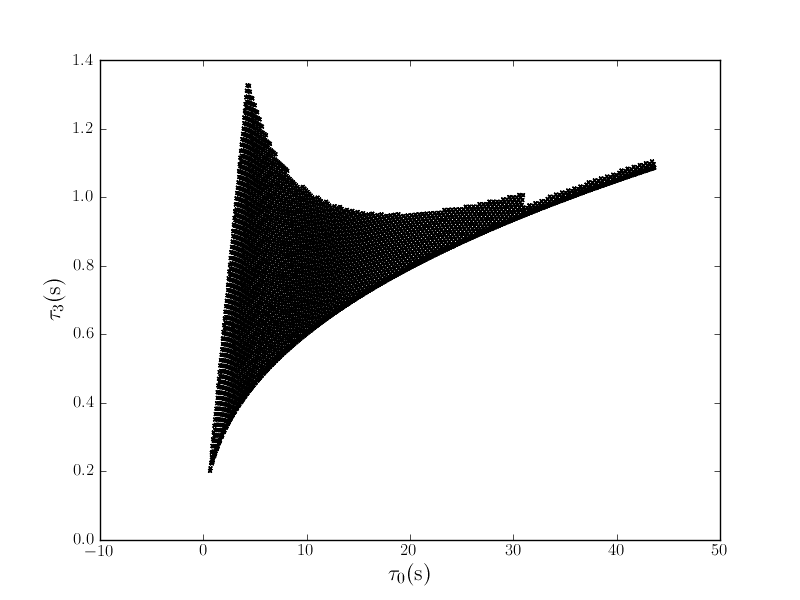
\includegraphics[width=2.6in]{figures/tau0tau3.png}}
\subfigure[In component mass.]{\label{fig:tmpltbank-mass1mass2}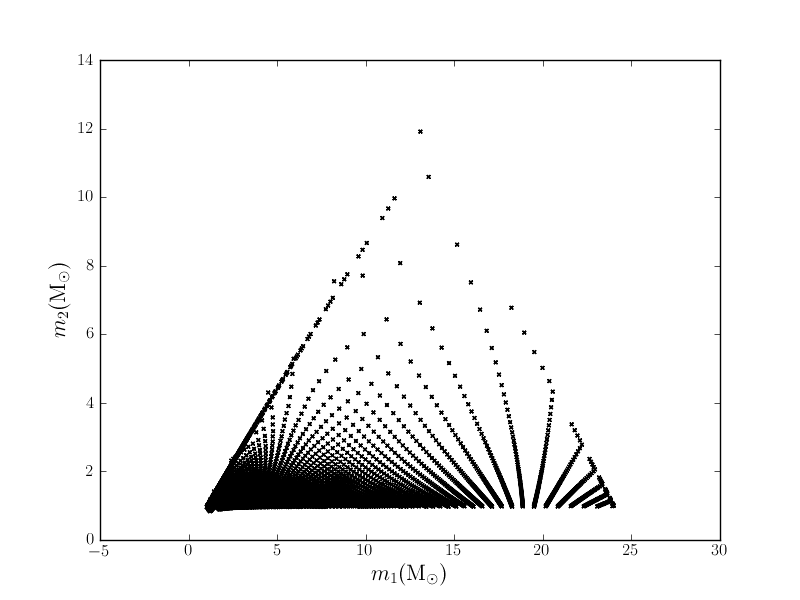
\includegraphics[width=2.6in]{figures/mass1mass2.png}}
\caption{
A typical template bank in $\tau_0,~\tau_3$ space and in $m_1,~m_2$ space
(where $m_1$ is the mass of the larger component mass). This plot generated
from a H1 template bank file in the $10\,240$ toy analysis. Note that the
templates are more evenly distributed in $\tau_0,~\tau_3$ space. As discussed
in section \ref{sec:tmpltbank}, this is because the parameter space is
approximately flat in $\tau_0$ and $\tau_3$ \cite{Owen:1995tm, Owen:1998dk,
Tanaka:2000, BBCCS:2006, hexabank}.  } \label{fig:template_bank} \end{figure}
\subsection{Injections}
\label{sec:inspinj}

Software injections are the \ac{CBC} group's way to check that our pipeline is
working.\footnote{As mentioned in section \ref{sec:PipelineRequirements}
hardware injections exist too. These are also used to check that the pipeline
is working. However, because we cannot perform the large number of hardware
injections needed for Monte Carlo simulations --- as we can with software
injections --- they are of limited use for tuning and efficiency studies.}
Since the number we can perform is only limited by computational power, we can
do a large number across a broad range of parameters and sky positions. Being
able to perform such Monte Carlo simulations allows us to test the efficiency
of our pipeline, tune parameters, and calculate rate limits to compare to
astrophysical expected rates.

Injections are only performed in injection \hipe~\acp{DAG}; these are later
combined with non-injection results by Pipedown. For example, in our toy
analysis, we have chosen to do one injection \ac{DAG}, which we labeled
\texttt{BNSINJ}. If we are performing an injection run then, prior to launching
first inspiral jobs, \hipe~runs \texttt{lalappps\_inspinj}. \texttt{Inspinj}
generates a list of injections to perform based on the input arguments. It does
not create the waveforms themselves; that is left to \texttt{lalapps\_inspiral}
(see below).

The configuration file determines how the injections are distributed in mass,
mass-ratio, sky-location, orientation, and time. For a given injection
\ac{DAG}, a minimum and maximum component mass are specified, along with a
maximum total mass. Additionaly, what mass parameter to distribute the
injections in must be specified. For \ac{S5} and \ac{S6} injections were chosen
to be distributed uniformly in component mass. How to distribute the location
of injections is also required. In \ac{S5} a galaxy catalogue was used for the
location distribution \cite{Collaboration:2009tt, Abbott:2009qj}; random
galaxies were chosen for an injection to occur in. For \ac{S6}, the range of
the detectors was large enough to ignore inhomogenities in the universe
\cite{ratesdoc}; thus in \ac{S6} the location distribution was changed to be
randomly distributed across the sky. The orientation of injections was
distributed uniformly across inclination angles for both \ac{S5} and \ac{S6}.

Injections are distributed randomly in time. However, to prevent too many
injections from occuring in the same period, a time-step and time-interval
argument are added. The time-step argument sets the average period of time
between each injeciton, and the time-interval sets the interval around that
time-step in which an injection is randomly placed. For example, in \ac{S6} the
time-step was set to $837\,$s and the time-interval was set to $300\,$s. This
means that if an injection occurs at time $t_0$, the next injection will be
chosen to randomly occur in the interval $(t_0 + 837) \pm 300\,$s.

We distribute injections in distance based on the range of the detectors. We
are most interested in the region around the network's \emph{horizon
distance},\footnote{Horizon distance is the furthest point the detectors can
detect. From the antenna pattern shown in Figure \ref{fig:antenna_pattern}, we
see that this point corresponds to a binar situated directly above or below the
detector, with an inclination angle of zero.} we as this is where the
efficiency quickly drops from $\sim1$ to $0$ (for a given false alarm rate).
Since the detectors' sensitivity is mass dependent, we adjust the domain of
distances in which to distribute injections according to the mass-range and
type of injections being performed. Injections may be distributed uniformly in
distance or in log distance. When we distribute uniformly in distance, we tend
to over populate the outer regions of the range, since volume grows as $r^3$.
If we distribute uniformly in log distance, we tend to over populate the inner
regions of the range. For this reason, two injection sets are typically done
for a single mass-range and injection type: one that is distributed linearly in
distance and one distributed uniformly in log distance. Prior to analysis, the
choice of injection ranges is based on a best-guess of what the range will be
from \ac{PSD} estimations at a single-detector \ac{SNR} of 8. Since we cannot
know the \emph{exact} range of the network of detectors until after the
analysis is complete, extra injection runs are done after the analysis. These
runs are set up to better target the range around the horizon distance so as to
have good statistics for upper-limit calculations.

The waveform generator used by \texttt{lalapps\_inspiral} has the ability to
create waveforms from several different template families, not just restricted
non-spinning \ac{pN} templates. Thus we check how well spinning waveforms are
recovered using our non-spinning template bank. This was done for both \ac{S5}
and \ac{S6} searches, as separate upper-limits were produced for spinning
\ac{NSBH} and \ac{BBH} systems. Additionally, we can check how well various
waveform families overlap with the \ac{pN} approximation we use for the
templates in the template bank. For example, in the \ac{S6} low-mass \ac{CBC}
search, \ac{NSBH} injections were generated using the EOBNR psuedo-4\ac{pN}
model \cite{Buonanno:2009qa}.

Each injection \hipe~\ac{DAG} will only draw from a single waveform family,
with a give range of parameters, and with a given random-number-generator seed.
To create a large number of injections, multiple injection runs are done; some
of these will have the same range of parameter, with only the random seed
changing. When \texttt{lalapps\_inspinj} runs in a given injection run, it
saves the list of injections to perform to a \texttt{sim\_inspiral} table that
lists the times, parameters, and waveform family of the injections to create.
(See section \ref{sec:sim_inspiral-process_tables} for more details about the
\texttt{sim\_inspiral} table.) This table is saved to an XML file with naming
convention:
\begin{center}
\texttt{HL-INJECTIONS\_\{SEED\}\_\{USER-TAG\}-\{GPS-START\}-\{DURATION\}.xml}
\footnote{The \texttt{HL} prefix on the \texttt{INJECTIONS} file is an
anachronism from when searches were only done between the two \ac{LIGO} sites.
The \texttt{sim\_inspiral} table actually contains injection information for
all the detectors in the search.}
\end{center}

\texttt{SEED} is number given as a seed to the random-number generator in
\texttt{inspinj} in the given \ac{DAG}. \texttt{USER-TAG} is the user-tag given
to each \hipe~\ac{DAG} by \ihope. As discussed in section
\ref{sec:hipe_overview}, the non-injection \ac{DAG} will be named
\texttt{FULL\_DATA} whereas each injection run will have a unique name to
distinguish it from the other injection runs. Unlike the \texttt{FULL\_DATA}
tag, the injections' \texttt{USER-TAG}s are set in the configuration file. For
example, since we have done one injection run in our toy analysis, we have two
unique user-tags: \texttt{FULL\_DATA} and \texttt{BNSINJ}. One
\texttt{INJECTIONS} file exists for each injection run; this file is loaded by
\texttt{lalapps\_inspiral} to insert the injections into the data.

\subsection{First Inspiral}
\label{sec:first_inspiral}

With the template bank and (for injection runs) list of injections generated,
\hipe~next runs \texttt{lalapps\_inspiral} to match filter the data
\cite{brown-2005-22}. One inspiral job exists for each \texttt{tmpltbank} job;
i.e., there is an inspiral job for each detector and for each analysis block.
\texttt{Inspiral} loads the frame cache and the template bank corresponding to
its block. Additionally, if \texttt{inspiral} is being run in an injection
\ac{DAG}, it will read in an \texttt{INJECTIONS} file.

\texttt{Inspiral} carries out the same data conditioning as \texttt{tmpltbank}
(in fact, they call the same code): data is read in, low- and high-pass
filtered, and resampled \cite{brown-2005-22, Allen:2005fk}. If
\texttt{inspiral} is given an injections file it will create the waveforms that
overlap its analysis time prior to data conditioning. Waveforms are generated
in the time-domain using the parameters stored in the \texttt{sim\_inspiral}
table and added directly to the data stream in memory. The data is then low-
and high-pass filtered and resampled. Note that \texttt{tmpltbank} does not
load injections. Instead, the same bank is used for both non-injection and
injection runs. While this introduces a subtle difference from the real
situation, the effect on the template bank is negligible, since the median
estimator is used, and since the number of injections in a block is limited by
the time-step and time-interval arguments given to \texttt{lalapps\_inspinj}.

After the data is conditioned and the \ac{PSD} estimated, \texttt{inspiral}
reads in a template from the \texttt{TMPLTBANK} file, generates it (in the
frequency domain), then match filters it with the data to create the (complex)
\ac{SNR} time series for the given template \cite{brown-2005-22, Allen:2005fk}.
This is repeated for each template in the bank file. For injection runs, an
optional argument \texttt{enable-inj-filter-only} can be turned out that causes
the \texttt{inspiral} to only filter segments containing an injection. This
cuts down on computational time and has no effect on the analysis, since we are
only interested in times around an injection (all other times are assumed to
return the same result as the non-injection run).

As discussed in Chapter \ref{ch:pipeline_principles} we identify triggers by
finding points where the \ac{SNR} ($\rho$) is at a maximum. Due to noise,
however, there will be multiple local maxima across the duration of a template.
We must therefore employ time-domain clustering on the \ac{SNR} so as to
associate a single trigger with an event. This is done by using the \emph{max
over chirp length} algorithm \cite{Brown}. Max over chirp length uses a sliding
time window to select triggers: for every point in time, a point is only kept
if there is no other point with a $\rho$ greater than it within the chirp
length of the template. Once a trigger is identified, the time at which it
occurs is associated with the \emph{coalescence}, or \emph{end-time}, $t_c$, of
the binary. If the \ac{SNR} of the trigger exceeds our desired \ac{SNR}
threshold, it is kept. The \ac{SNR} threshold is set in the configuration file;
for both \ac{S5} and \ac{S6} it was set to 5.5.

Due to the high overlap between templates in the bank, a single event can
create triggers across multiple templates. In order to associate a single
trigger with a single event, we also need to cluster across the bank.
\texttt{lalapps\_inspiral} offers two options: time-window clustering, and
\emph{TrigScan} \cite{SenguptaTrigScan}. The time-window clustering is the
simplest of the two: the time series is split up into windows with a set
duration (determined in the configuration file). Within each window, the
trigger with the largest \ac{SNR} is kept while all others are discarded. This
method has the advantage of being simple, and it garauntees that the trigger
rate in a single detector will not exceed one per the window duration. However,
choosing the size of the window is difficult and somewhat arbitrary. Different
templates have varying impulse responses and will ``ring" for varying amounts
of time depending on the strength of a signal or glitch. Thus the window is
unlikely to cause only one trigger to be associated with one event.
Additionally, a glitch that creates triggers at in the high-mass region of the
template bank can cluster away a true signal candidate that created triggers at
the low-mass region of the bank,\footnote{Refer to figure
\ref{fig:template_bank}.} even though the glitch and the signal candidate look
nothing like each other.

A more sophistcated approach is to use TrigScan clustering
\cite{SenguptaTrigScan, Keppel:thesis}. Rather than simply use the
time-dimension, trigscan also pulls in information about the parameters of the
templates to cluster. The method is similar to that of coincidence testing,
discussed in section \ref{sec:coincidence_test}: for a given trigger, TrigScan
constructs an e-thinca ellipsoid\footnote{Recall from section
\ref{sec:coincidence_test} that an e-thinca ellipse defines the volume of
parameter space around a template for which a signal with the template's
parameters will fall to some probability \cite{Robinson:2008}.} with size
$\epsilon_{ts}$ around the trigger using the bank metric computed by
\texttt{tmpltbank}. (The value of $\epsilon_{ts}$ is determined from tuning
studies and is set in the configuration file).) It then collects all triggers
that fall within that ellipse. Ellipses are then constructed around each new
trigger found, and more triggers are collected around them. This continues
until no more triggers can be found within any ellipse. The trigger with the
largest \ac{SNR} amongst the collected triggers is kept and the others are
discarded \cite{SenguptaTrigScan, Keppel:thesis}. By involving parameter
information this method has the advantage that it can cluster on a good
candidate on in one region of the template bank without being affected by a
glitch in another region of the template bank. Also, since time is incorporated
in the metric used to construct the e-thinca ellipse, the size of the cluster
window in the time dimension will adjust for each template.\footnote{Basically,
shorter-duration templates will have larger time windows since we cannot
localize their parameters with as high confidence as we can longer-durationt
templates \cite{SenguptaTrigScan}.} The disadvantage to this method is that it
does not gaurauntee a maximum trigger rate. (This proved to be a problem for
\ac{S6}; see Chapter \ref{ch:s6_results} for details.)

All surviving triggers are saved to the \texttt{sngl\_inspiral} table with
their template parameters, \ac{SNR}, and \emph{end time}. The ``end time" is
the point when the frequency in \ac{pN} approximation goes to infinity
\cite{Brown}; it is how we identify when a trigger occurs. This table is stored
in a XML file; the naming convention used is:
\begin{center}
\texttt{\{IFO\}-INSPIRAL\_FIRST\_\{USER-TAG\}-\{GPS-START\}-\{DURATION\}.xml}
\end{center}
All of the \texttt{FULL\_DATA INSPIRAL\_FIRST} files that are created in our
analysis are shown in Figure \ref{fig:segment_plot_full}. There will be an
equal number of \texttt{BNSINJ} files, the only difference in the names being
the \texttt{USER-TAG}.

\texttt{lalapps\_inspiral} is also used to calculate $\chi^2$ values for
triggers. However, since this is not used until the second stage of the
pipeline, we withold discussion of this until secton \ref{sec:second_inspiral}.

\subsection{First Coincidence}
\label{sec:first_thinca}

Now that we have lists of single-detector triggers we can perform the
coincidence test across detectors. This is done by \texttt{lalapps\_thinca}
\cite{Keppel:thesis}. Each \texttt{thinca} job reads in multiple
\texttt{inspiral} files. The number and duration of \texttt{thinca} jobs is
determined by \emph{coincidence times}. A coincident segment of time is
determined by the number of detectors that are operational --- i.e., in Science
mode and not vetoed --- during that segment. For example, if H1 and L1 are
operating for the same period of time, we refer to this as H1L1-coincident
time. One \texttt{thinca} job will be created for every contiguous coincidence
time. This is illustrated in Figure \ref{fig:segment_plot_full}. Only H1 and L1
were analyzed for the first $\sim1700\,$s of the analysis. Thus, one instance
of \texttt{thinca}, or \emph{job}, is run for this period. At GPS time
$967230087$ Virgo turns on, and for the next $2176\,$s all three detectors are
analyzed. This results in another \texttt{thinca} job being created for this
H1L1V1-coincidence time. Afterward, L1 turns off, and so an H1V1
\texttt{thinca} job is created for the next $1755\,$s. This is again followed
by a period of H1L1V1-coincident time.

Unlike \texttt{tmpltbank} and \texttt{inspiral} jobs, there is no minimum
required duration of contiguous analysis time for \texttt{thinca}; in
principle, a \texttt{thinca} job could be as short as one second. A maximum
duration of $3600\,$s is imposed to protect against memory errors. If a period
of coincidence time is greater than $3600\,$s and less than $7200\,$s, however,
the time will be evenly split between two \texttt{thinca} jobs. This can be
seen in the last H1L1V1-coincident segment in Figure
\ref{fig:segment_plot_full}. Note that no overlap is applied between
\texttt{thinca} jobs.

\texttt{Thinca} performs the coincidence test using the method outlined in
section \ref{sec:coincidence_test}: it constructs an e-thinca ellipsoid around
each trigger with size $\epsilon_{\mathrm{thinca}}$ using the metric components
computed by \texttt{tmpltbank} \cite{Robinson:2008}. The size of
$\epsilon_{\mathrm{thinca}}$ is a tunable parameter and is set in the
configuration file \cite{Keppel:thesis}. Single-detector triggers are
considered coincident if their e-thinca ellipsoids overlap. A single trigger
can take part in multiple coincidences if it overlaps with multiple triggers. A
triple (or higher) coincidence can only occur if all three triggers in each
detector overlap with each other. If one trigger overlaps with the other two,
but those two do not overlap with each other, two double coincidences will be
created.

Any single-detector triggers found to be in coincidence with a trigger with at
least one other detector are saved to the \texttt{sngl\_inspiral} table in the
output XML file.  One XML file is created for each \texttt{thinca} job. Note
that this means a single \texttt{thinca} XML file will contain triggers from
multiple detectors; how these are stored in the \texttt{sngl\_inspiral} table
is discussed in section \ref{sec:data_storage}. The naming convention for first
coincidence files is:
\begin{center}
\texttt{\{IFOS\}-THINCA\_FIRST\_\{USER-TAG\}-\{GPS-START\}-\{DURATION\}.xml}
\end{center}
\texttt{IFOS} is the coincidence time the \texttt{thinca} file
covered; it is not necessarily the coincidence types stored in the
file.\footnote{For example, an H1L1V1-coincident time file will have prefix
\texttt{H1L1V1}, yet can contain up to four coincidence types: H1L1, H1V1,
L1V1, and H1L1V1.} Any single-detector trigger that is not coincident with any
other detector is discarded.

\texttt{Thinca} also has the ability to apply higher-category vetoes and do
time slides. As this is not done until the second stage, we withold discussion
of this until section \ref{sec:second_thinca}.

\subsection{Trigbank}
\label{sec:tribank}

The completion of first coincidence concludes the first stage of the
\hipe~pipeline. To carry out the second stage of the pipeline, we must first
gather all surviving triggers in preparation for the second run of
\texttt{lalapps\_inspiral}. This is done by \texttt{lalapps\_trigbank}
\cite{brown-2005-22}. The number of \texttt{trigbank} jobs is determined by the
number of single-detector analysis blocks and the number of coincidence times.
Within each analysis block, a separate \texttt{trigbank} job is created for
each coincidence time that exists in that block and for each detector. For
example, in our toy analysis, the first H1 analysis block overlaps
H1L1-coincident time and H1L1V1-coincident time. Therefore, two
\texttt{trigbank} jobs are created for H1 during this time, one for each
coincidence time.

Each \texttt{trigbank} job loads all first \texttt{thinca} files of a given
coincidence time that overlap its analysis block. All triggers from a single
detector are picked out of the \texttt{thinca} files and redundancies are
removed. We do this because the same template will have multiple entries in the
\texttt{sngl\_inspiral} table if it generated multiple single-detector triggers
across the analysis block. As these files will eventually be loaded by
\texttt{inspiral} to perform match filtering (see section
\ref{sec:second_inspiral}, below), we only wish to keep one entry for the
template, else \texttt{inspiral} will filter the same template multiple times.
The results are then saved to a \texttt{sngl\_inspiral} table in a
\texttt{TRIGBANK} file; the naming convention is:
\begin{center}
\texttt{\{IFO\}-TRIGBANK\_SECOND\_\{COINCIDENT-TIME\}\_\{USER-TAG\}-\{GPS-START\}-\{DURATION\}.xml}
\end{center}
\texttt{COINCIDENT-TIME} is the coincident time from which the triggers in the file
came. By adding this tag we ensure that a different file exists for each
coincidence time. Figure \ref{fig:segment_plot_full} shows all of the
\texttt{FULL\_DATA TRIGBANK} files created in our toy analysis.

\subsection{Second Inspiral}
\label{sec:second_inspiral}

After the trigbank files have been generated, \texttt{lalappps\_inspiral} is
run again \cite{brown-2005-22}. As with first \texttt{inspiral}, the second
instance of \texttt{inspiral} loads the strain data from the frame files,
conditions the data, adds injections (for injection runs), and match filters
the data. There are two important differences: first, $\chi^2$ is now computed
along with \ac{SNR}, and a $\chi^2$ threshold and $r^2$ veto are applied to
triggers.  Second, rather than load a \texttt{TMPLTBANK} file, a
\texttt{TRIGBANK} file is used. Since the \texttt{TRIGBANK} file only contains
the single-detector triggers that passed first coincidence, this reduces the
number of triggers for which \texttt{inspiral} will have to calculate a
$\chi^2$ value.

$\chi^2$ is computed for any trigger that exceeds the \ac{SNR} threshold. (Note
that triggers have been defined before this happens; i.e. the max-over
chirp-length algorithm is still based solely on \ac{SNR}.) As per the equations
outlined in section \ref{sec:chisq} of Chapter \ref{ch:pipeline_principles},
this is done by breaking the template up into bins of equal power, match
filtering each bin individually, and comparing the \ac{SNR} in each bin to the
expected \ac{SNR} in a single bin \cite{Allen:2004, Allen:2005fk}. The number
of bins used is set in the configuration file. For \ac{S5} and \ac{S6} 16 bins
were used, making the number of degrees of freedom equal to 30. This process is
computationally expensive \cite{Allen:2005fk}; hence it is only used for
triggers that survive first coincidence. Once the $\chi^2$ value for a trigger
is computed, the $\chi^2$ threshold is applied. While the exct value of the
$\chi^2$ threshold is \ac{SNR} dependent, the value of $\chi_*^2$ (see equation
\ref{eqn:chisq_threshold} in Chapter \ref{ch:pipeline_principles}) is a
tuneable parameter \cite{Keppel:thesis} that is set in the configuration file.
If a trigger has a $\chi^2$ that exceeds the $\chi^2$ threshold, it is
discarded. \texttt{Inspiral} also computes an $r^2$ value for each trigger
across a period of time that is also set in the configuration file (see
equation \ref{eqn:rsq_veto} in Chapter \ref{ch:pipeline_principles}). If the
$r^2$ value exceeds a threshold $r_*^2$ determined in the configuration file,
the trigger is discarded. For values of $\chi_*^2$, $r_*^2$, and the size of
the $r^2$ window used for \ac{S5} see \cite{Rodriguez:2007, Keppel:thesis}. The
same values were used for \ac{S6}. \texttt{Inspiral} does not compute effective
\ac{SNR} nor New \ac{SNR}. Instead, the $\chi^2$ value for surviving triggers
and the number of degrees of freedom are saved to the \texttt{sngl\_inspiral}
table along with the triggers' other information (\ac{SNR}, template
parameters, end time). Later programs use this information to compute effective
or New \ac{SNR} as needed (c.f. section \ref{sec:thinca_to_coinc}).

Clustering across the bank (either by the hard-window method or TrigScan) is
still based on \ac{SNR}. However, because this occurs after the $\chi^2$ and
$r^2$ vetoes are applied, the trigger that survives bank clustering may not be
the same as in first \texttt{inspiral}. For example, a glitch or signal may
cause a trigger with a large \ac{SNR} but a poor $\chi^2$. If this template had
the largest \ac{SNR} across the bank, it would have been selected in the first
stage. However, if the template's $\chi^2$ or $r^2$ value exceeds the veto
threshold, it will not survive to the bank clustering phase, and so another
template will be selected. 

As can be seen in Figure \ref{fig:segment_plot_full}, one second
\texttt{inspiral} job is run for every \texttt{trigbank} file. Since there are
many more \texttt{trigbank} files than \texttt{tmpltbank} files, this may seem
to defeat the purpose of limiting the number of triggers for which $\chi^2$ is
calculated. However, templates in a given \texttt{trigbank} file are only
filtered through segments that overlap with the corresponding \texttt{thinca}
file  (the entire analysis block is used for to compute the \ac{PSD}
\cite{brown-2005-22}). For example, in our toy analysis, there are two
\texttt{trigbank} files --- and therefore two second \texttt{inspiral} jobs ---
for the first H1 analysis block. This was because part of the way through the
block, V1 turned on, and so we switched from H1L1-coincident time to
H1L1V1-coincident time. The second \texttt{inspiral} job that reads in the H1L1
\texttt{trigbank} file in this analysis block will only match filter the
segments that overlap the H1L1-coincident time (which is the first $1672$
seconds of the block). Likewise, the second second-\texttt{inspiral} job in
this block, which is associated with the H1L1V1 \texttt{trigbank} file, will
only match filter the segments that overlap H1L1V1-coincident time (which is
the last $376$ seconds). For this reason, the naming convention for second
\texttt{inspiral}'s output XML files is:
\begin{center}
\texttt{\{IFO\}-INSPIRAL\_SECOND\_\{COINCIDENT-TIME\}\_\{USER-TAG\}-\{GPS-START\}-\{DURATION\}.xml}
\end{center}
By limiting the filtering in this manner we minimize the number of triggers for
which we need to compute a $\chi^2$ value \cite{brown-2005-22}.

\subsection{Second Coincidence}
\label{sec:second_thinca}

Since many triggers will have failed the $\chi^2$ and $r^2$ vetoes in second
\texttt{inspiral} (and since slightly different templates may have taken their
place) we must again perform the coincidence test \cite{Keppel:thesis}. This is
carried out by \texttt{lalapps\_thinca} with many of the same arguments as
before. In fact, the CAT1, zero-lag coincidence job will perform exactly the
same operations as its first stage counterpart; even the start/end times (which
correspond to the coincidence times) will be the same. The only difference is
the second stage coincidence will read in the corresponding
\texttt{INSPIRAL\_SECOND} files.

It is at this point that we perform time-slides and apply higher-category
(i.e., $>$ CAT1) vetoes. This results in several additional \texttt{thinca}
jobs than were carried out at first stage. Specifically, for a non-injection
run, there will one zero-lag and one slide \texttt{thinca} job for each
category of veto analyzed.\footnote{Although there are, in principle, up to
four categories of vetoes --- see table \ref{tab:veto_cats} --- not all of them
have to be analyzed by \hipe. The specific categories that we wish to analyze
are determined by the configuration file. For example, note that in Figure
\ref{fig:segment_plot_full} there are no CAT4 \texttt{THINCA\_SECOND} files.}
We do not perform slides for injection runs, but we do apply higher vetoes.

Higher category vetoes are applied by feeding \texttt{lalapps\_thinca} an ASCII
file containing the list of veto segments to apply for a given detector (and by
adding a \texttt{--do-veto} argument). These ASCII files are created by
\ihope~at run-time from the veto XML files created by
\texttt{ligolw\_segments\_from\_cats},\footnote{\texttt{Thinca} does not read
the XML files directly because it was written several years before
\texttt{ligolw\_segments\_from\_cats}. Rather than try to adjust
\texttt{thinca} to read the new XML files, we found it easier to simply convert
the XML to ASCII format.} and are stored in the \texttt{segments} directory. A
separate ASCII file is given to \texttt{thinca} for each detector. If a veto
file for a detector is specified, \texttt{thinca} loads it, then removes all
triggers from the given detector that have end times intersecting the veto
segments. This is done prior to performing the coincidence test. As mentioned
above, vetoes are applied cumulatively. Thus, the CAT2 veto file will contain
the union of category 1 and 2 veto segments; CAT3, the union of 1, 2, and 3;
etc. For this reason, \texttt{thinca} only needs to load one veto file per
detector per job.

Slides are carried out by giving \texttt{thinca} a \texttt{--num-slides}
argument, followed by arguments giving the relative offset to apply for each
detector. \texttt{Thinca} uses these arguments to construct offset vectors for
each slide. The offset values for each detector in a given slide are determined
by the slide number and the relative offsets of the detectors. For example, if
the H1 offset is 0 (set via the \texttt{--h1-slide} argument), the L1 offset is
5 (via \texttt{--l1-slide}), and V1 offset is 10 (\texttt{--v1-slide}), then
for the third slide, the offset vector will be:
\begin{equation}
\label{eqn:example_offsetvec}
\vec{\mathcal{O}}_3 = [\Delta t_{\mathrm{H1}} ~ \Delta t_{\mathrm{L1}} ~ \Delta t_{\mathrm{V1}}] = [0\,\mathrm{s} ~ 15\,\mathrm{s} ~ 30\,\mathrm{s}] 
\end{equation}
The \texttt{num-slides} argument sets the total number of slides to perform.
The number of slides will be twice the value given by this argument: one set of
forward slides, and one set of backward slides. For example, if
\texttt{num-slides} is 20, 40 total slides will be created: 20 slides with
positive offsets and 20 slides with negative offsets. The number of slides to
perform, and the offset for each detector is set in the configuration file. For
both \ac{S5} and \ac{S6}, the relative offset between the Hanford detectors and
L1 was $5\,$s; the relative offset was $10\,$s between the H1 and V1 in
\ac{S6}. H1 and H2 were not slid with respect to each other (i.e., their
relative offset was 0 for all slides) due to correlated noise between them (see
Chapter \ref{ch:s5_results} for details). In both \ac{S5} and \ac{S6}, 100
slides were used (50 forward slides and 50 backward). These could be increased
if we had a particularily loud coincident trigger; see Chapter
\ref{ch:s6_results} for more details. 

Both the \texttt{num-slides} and offset arguments must be integers. This means
that \texttt{thinca} cannot perform slides with offsets that are fractions of a
second. Furthermore, due to the way \texttt{thinca} constructs the offset
vectors, it is not possible to mix positive offsets with negative, nor is it
possible to have two separate vectors in which two of the detectors have the
same offset (unless the two detectors have the same relative offset). For
example, \texttt{thinca} cannot create the vectors $[\mathrm{H1} =
0\,\mathrm{s} ~ \mathrm{L1} = 5\,\mathrm{s} ~ \mathrm{V1} = 10\,\mathrm{s}]$
and $[\mathrm{H1} = 0\,\mathrm{s} ~ \mathrm{L1} = 5\,\mathrm{s} ~ \mathrm{V1} =
20\,\mathrm{s}]$. This limits the total number of slides \texttt{thinca} can
perform for times in which there are more than two coincident detectors.

For each slide, \texttt{thinca} adds the offsets to the end times of the
single-detector triggers then performs the coincidence test. This is done after
vetoes are applied, so that higher-category vetoes are effectively slid around
with the offset, too. Slides are performed on a \emph{ring}: triggers that are
slid past the end time of the \texttt{thinca} job are placed at the beginning
of the time. This means that a \texttt{thinca} slide job does not have to load
triggers from any other segment. It also means that triggers occuring in
single-detector time cannot be slid into coincidence time. Thus we are safe
discarding triggers that occur during single-detector time after the first
stage coincidence test. Since there is no minimum required duration for a
\texttt{thinca} file, this can mean that some slides will be redundant if a
file is too short. Studies have shown that this is rare, however, and so it has
little effect on the background analysis.

The naming conventions for second \texttt{thinca} output XML files are:
\begin{center}
\footnotesize{\texttt{\{COINCIDENT-TIME\}-THINCA\_SECOND\_\{COINCIDENT-TIME\}\_\{USER-TAG\}-\{GPS-START\}-\{DURATION\}.xml}}
\end{center}
for the CAT1 zero-lag files, and:
\begin{center}
\footnotesize{\texttt{\{COINCIDENT-TIME\}-THINCA\_SECOND\_\{COINCIDENT-TIME\}\_\{USER-TAG\}\_CAT\_\{N\}\_VETO-\{GPS-START\}-\{DURATION\}.xml}}
\end{center}
for the N$\th$-higher veto category.\footnote{Note that the second
\texttt{COINCIDENT-TIME} in the naming convention is unnecessary; it is simply a relic
of the \texttt{trigbank} and second \texttt{inspiral} naming conventions and
has no other meaning.} Slide files follow the same convention, except that
\texttt{THINCA\_SECOND} is replaced with \texttt{THINCA\_SLIDE\_SECOND}.

One important final note: by definition, when an detector is vetoed, it is no
longer considered to be ``on." This means that when we apply the
higher-category vetoes, coincidence times will change. For instance, if a
category-2 L1 veto comes on for $t$ seconds during H1L1V1-coincident time, then
at CAT2 (and all higher cumulative categories) that period of time is now
H1V1-coincident time.  The same rule applies to time slides. Second
\texttt{thinca} files, however, are grouped by whatever the coincidence time
was at CAT1, and this does not change after vetoes are applied (we seen this in
Figure \ref{fig:segment_plot_full}: all the \texttt{THINCA\_SECOND} files have
the same start and end times across all veto categories). This means that for
higher veto categories, a \texttt{THINCA\_SECOND} file will contain multiple
coincidence times. Unfortunately, \texttt{thinca} does not store which triggers
fall in which coincidence times, nor does it store the duration of each of the
coincidence times in its output file. As discussed in Chapter \ref{ch:far},
knowing the start and end of coincidence times is important information:
uncombined \acp{FAR} are computed for each coincidence type, and \acp{FAR} are
not combined across coincidence time. Thus later programs must re-apply the
vetoes to sort out the triggers and times. This is done by
\texttt{ligolw\_thinca\_to\_coinc}, which is the first program to run in
Pipedown (see section \ref{sec:PipedownDetail}).

\begin{figure}[hp]
\center
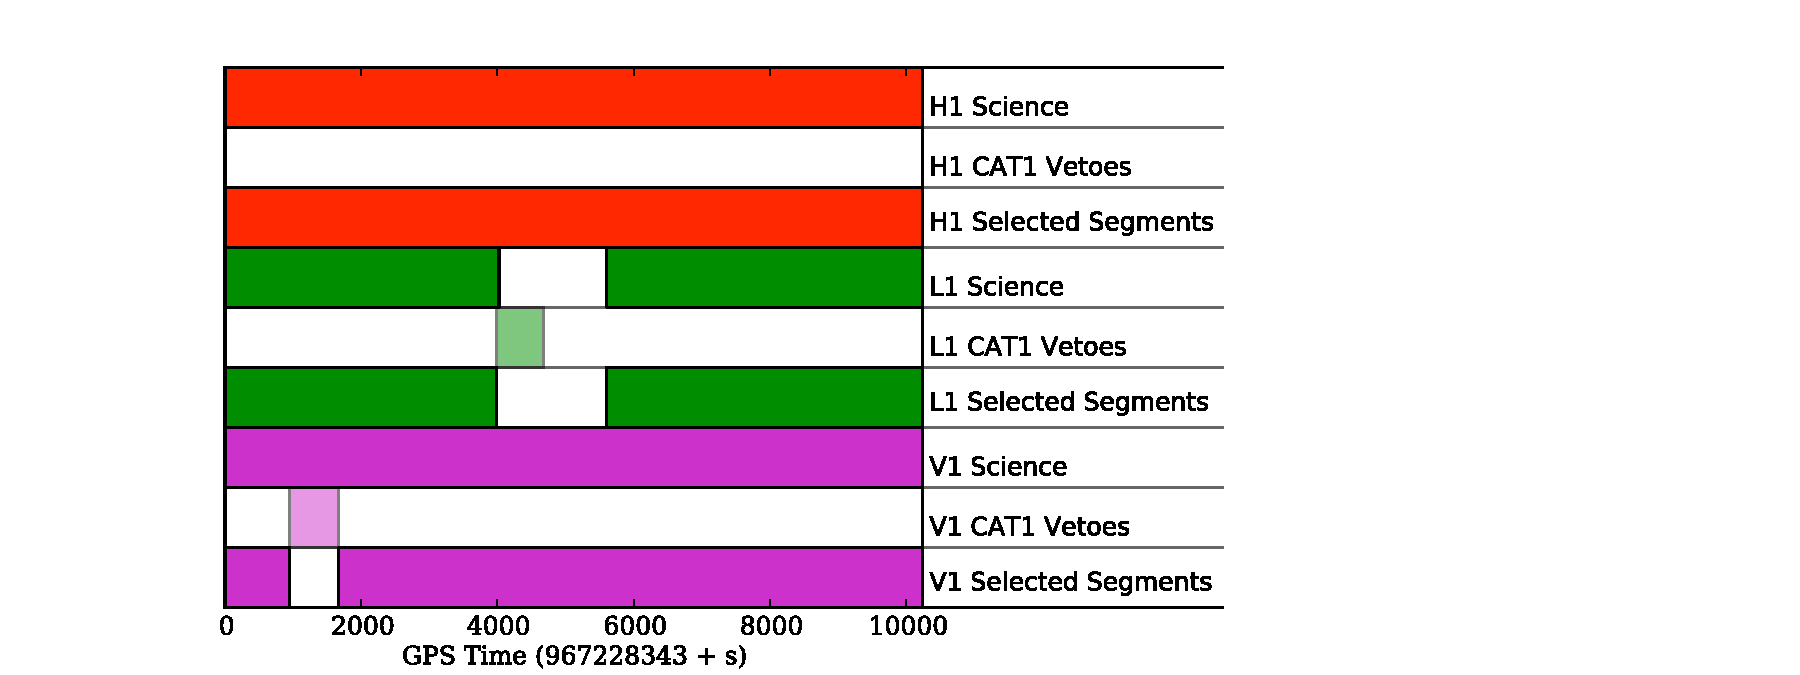
\includegraphics[width=6in]{figures/segment_plot_science-selected.pdf}
\caption{
The Science, category 1 vetoes, and selected segments of H1, L1, and V1 between
GPS times 967228343 and 967238583.
}
\label{fig:science-selected_segs}
\end{figure}

\begin{figure}[hp]
\center
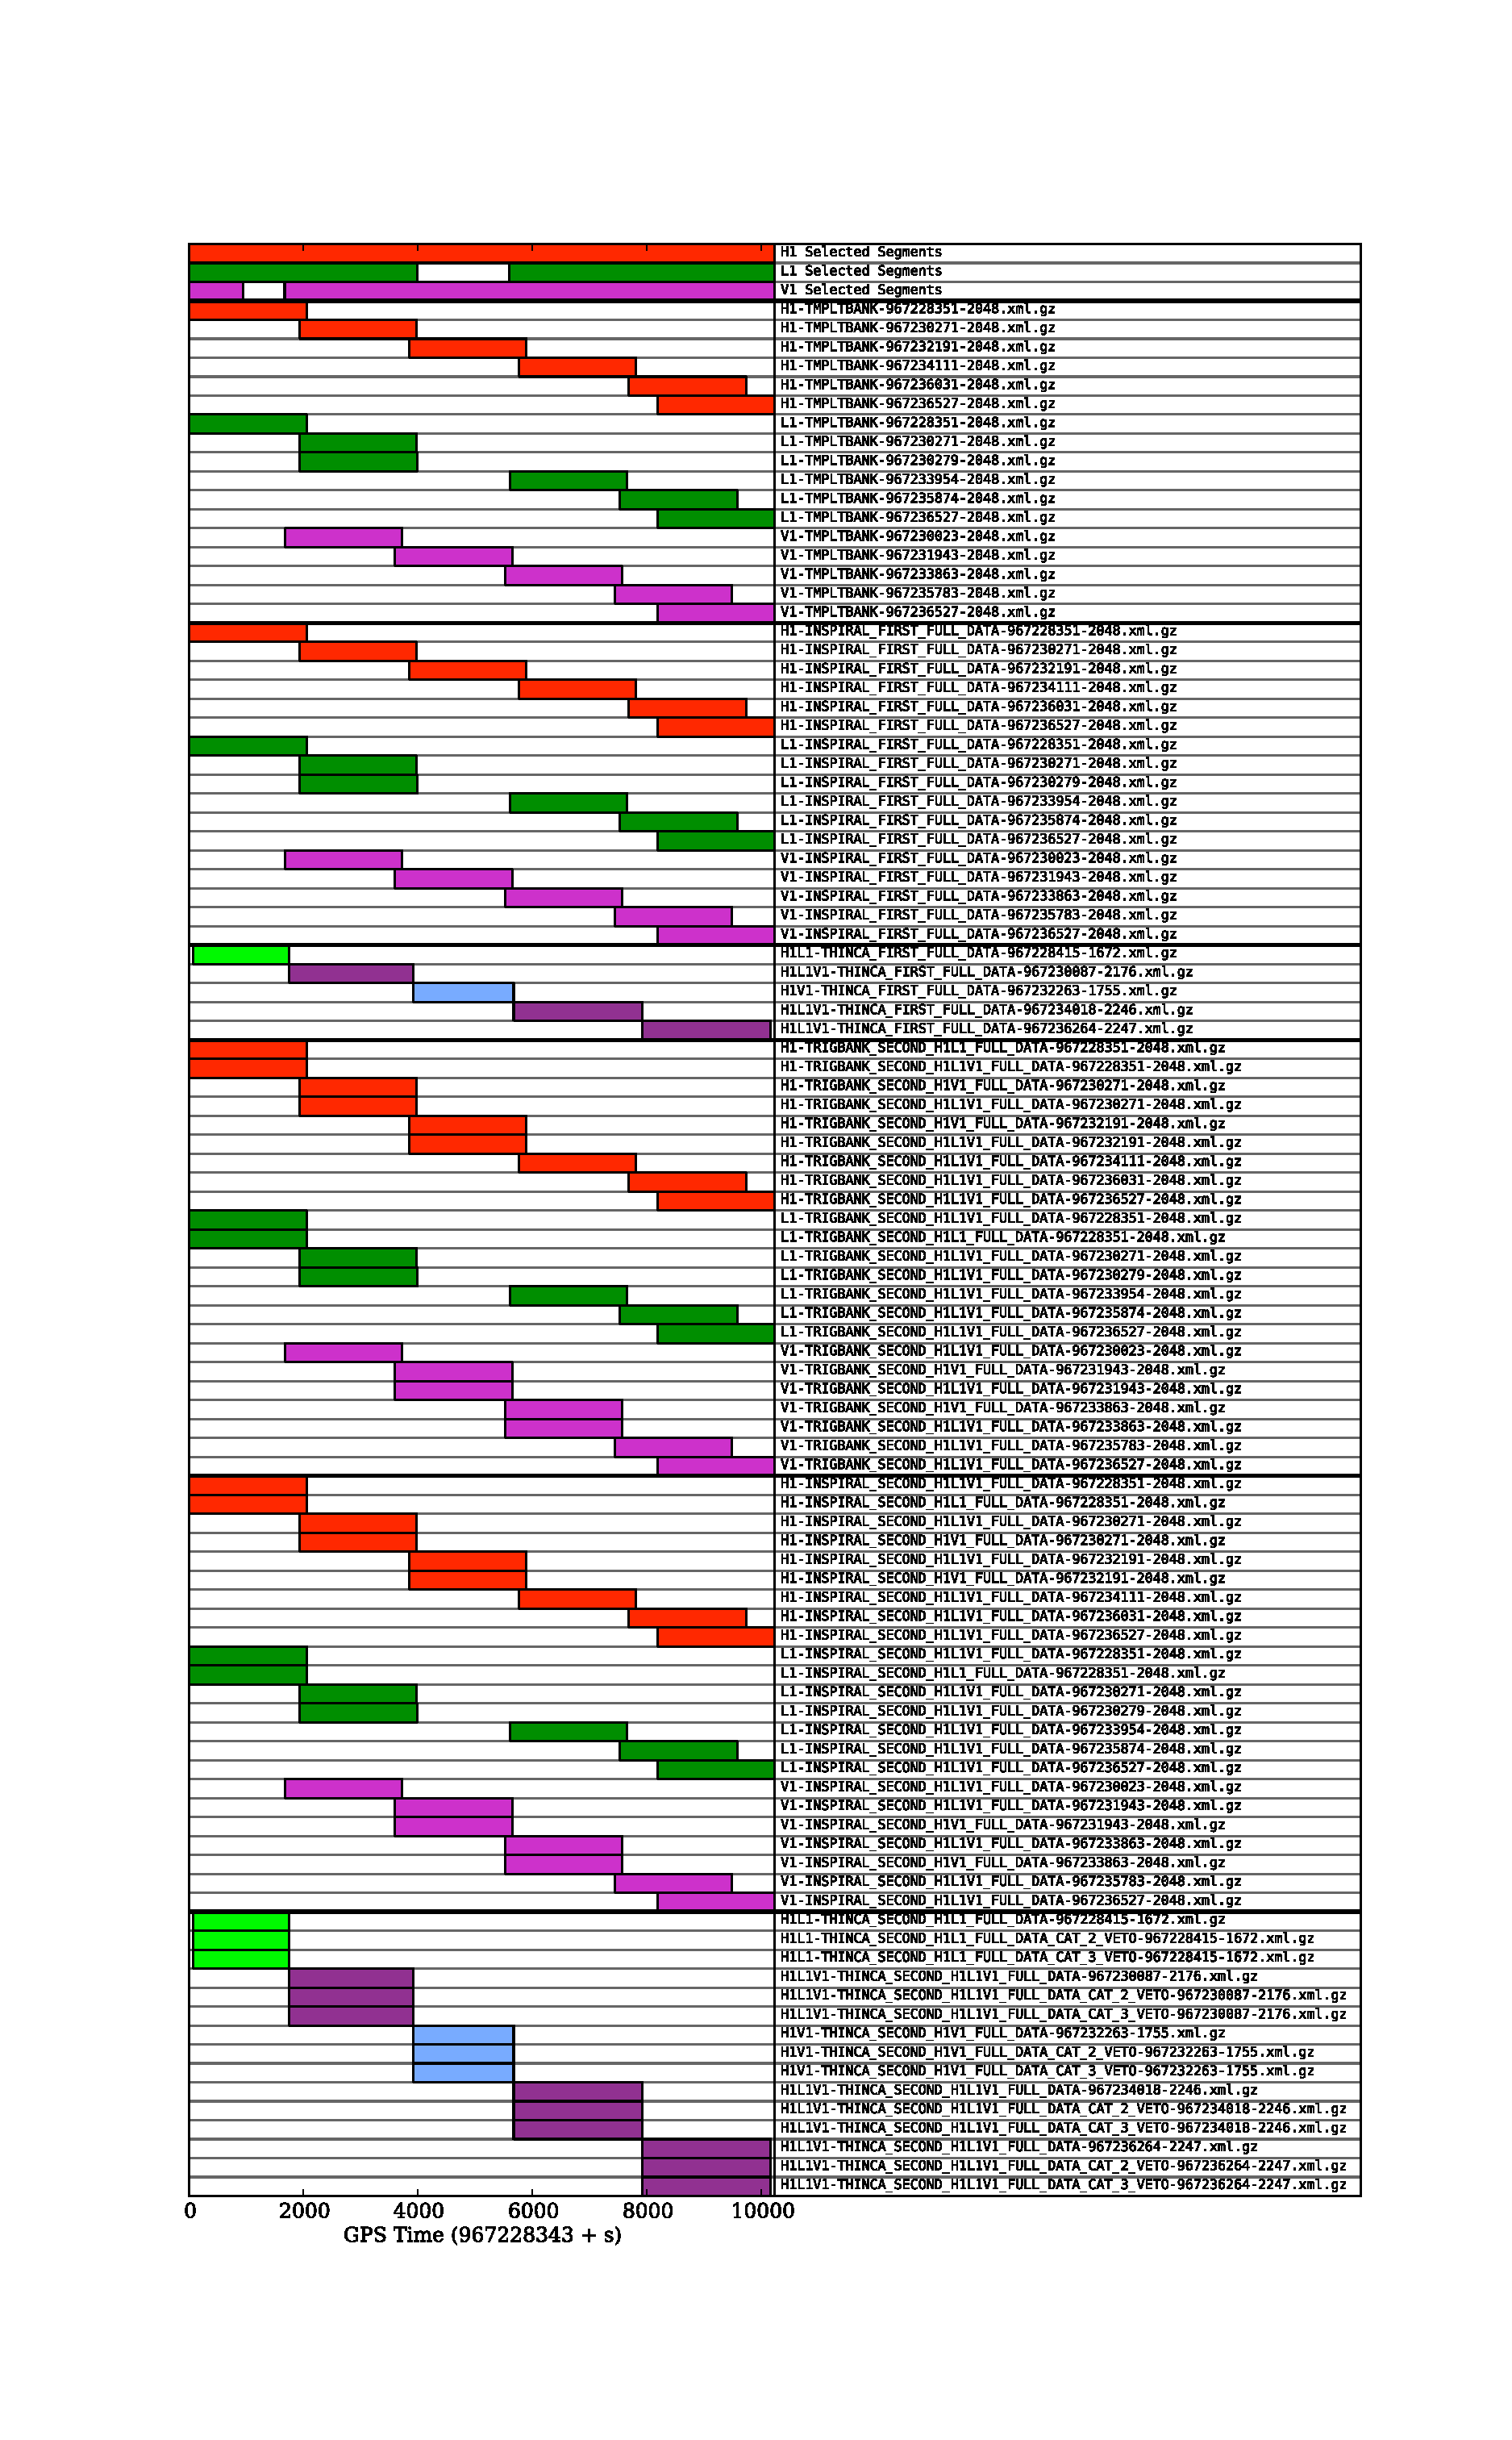
\includegraphics[height=8.5in]{figures/segment_plot_selected_segs-thinca_second.pdf}
\caption{
The selected segments and all zero-lag \texttt{FULL\_DATA} files created by
\hipe for the segments shown in Figure \ref{fig:science-selected_segs}.}
\label{fig:segment_plot_full}
\end{figure}

\section{Data Storage}
\label{sec:data_storage}

Before stepping through Pipedown, we pause to detail the table structure used
to store triggers in files. Table structure is central to Pipedown: part of its
purpose is to convert from older table structures to newer, more convenient
ones, and all the programs Pipedown runs take advantage of these newer tables.
We begin by reviewing the \texttt{sngl\_inspiral} table, and how this was used
to store data up to this point.

\subsection{The \texttt{sngl\_inspiral} Table}

As discussed above, the \texttt{sngl\_inspiral} table is the table used to
store data by nearly every \hipe~program: \texttt{lalapps\_tmpltbank},
\texttt{lalapps\_inspiral}, and \texttt{lalapps\_thinca} all use it to store
template and both single-detector- and coincident-trigger information.
Consequently, the \texttt{sngl\_inspiral} table has a large number of columns
to store all needed data. Table \ref{tab:sngl_inspiral} shows some of the
relevant columns used for the \ac{CBC} analysis and their purpose. There are
several extra columns not discussed here.\footnote{To see all current columns
of the \texttt{sngl\_inspiral}, as well as any other table discussed in this
section, see the \texttt{lsctables.py} code in the LALSuite repository. A URL
to the repository is given in section \ref{sec:other_tables}.}

Each row in the \texttt{sngl\_inspiral} table represents a single trigger or
template in a single detector. Associated with each row is an
\texttt{event\_id} to uniquely identify each event. This provides a convenient
way to retrieve information about a template or single-detector trigger.
Coincident information is more difficult to store, however, since coincidence
requires grouping rows together. Since the \texttt{sngl\_inspiral} table was
the only available way to store trigger data in a file when
\texttt{lalapps\_thinca} was written, a method was devised to encode
coincidence in the \texttt{event\_id}. The id was set to be 18 digits long. The
first (starting from the left) 9 digits were the GPS time of the trigger. The
next 4 digits gave the slide that the coincidence was from, where $0000$ was
zero-lag. The last 5 digits formed a counter that assigned a unique number to
each coincidence. For example, the first coincident trigger in H1L1-coincident
time in the first slide of our toy analysis has \texttt{event\_id}:
\begin{equation*}
\underbrace{967228415}_{\text{GPS time}}\underbrace{0001}_{\text{slide number~}}\underbrace{00001}_{\text{~event counter}}
\end{equation*}
Any rows that had \texttt{event\_id}s with the same last 9 digits --- i.e., if
the slide number and event counter matched --- are coincident triggers.

\subsection{The \texttt{sim\_inspiral} and \texttt{process} Tables}
\label{sec:sim_inspiral-process_tables}

Two other tables used by \hipe, as well as Pipedown, are worth mentioning: the
\texttt{sim\_inspiral} and \texttt{process} tables. The \texttt{sim\_inspiral}
table is similar to the \texttt{sngl\_inspiral} table. Instead of storing
triggers, it stores lists of injections. Some of the columns of the table are
shown in Table \ref{tab:sim_inspiral}. The table is indexed by the
\texttt{simulation\_id}. This id is simply a number: no information is stored
in it, as it is with the \texttt{event\_id}.

Note that both the \texttt{sim\_inspiral} and \texttt{sngl\_inspiral} table (as
well as many other tables) have \texttt{process\_id} columns. These are used to
map their entries to the \texttt{process} table. This table --- the columns of
which are shown in table \ref{tab:process} --- is used to store relevant
information about the program that created the entry. Associated with the
\texttt{process} table is the \texttt{process\_params} table, which stores the
arguments and values given to the program at run-time. For example, all the
injections created by a single instance of \texttt{lalapps\_inspinj} will have
the same \texttt{process\_id} in the \texttt{sim\_inspiral} table. These will
all point to a single entry in the \texttt{process} table and multiple entries
(one for each argument given to \texttt{lalapps\_inspinj}) in the
\texttt{process\_params} table. These tables are useful for troubleshooting
problems and verifying the correct program versions were used when an analysis
was run. They are also used to associate a set of injections with a given
injection \texttt{USER-TAG}; see section \ref{sec:Pipedown-injBranch} for details.

\subsection{Coinc Tables}
\label{sec:coinc_tables}

There were a few problems with using the \texttt{sngl\_inspiral} table to store
coincident information. First, the number of coincident events in a single file
could not exceed $99\,999$, or else the event counter would spill over into the
slide number. Likewise, no more than $9999$ slides could be stored in a single
file. Third, it consumed more memory than necessary. If a single-detector
trigger formed coincidences in multiple slides (as is often the case), multiple
entries would have to be created in the \texttt{sngl\_inspiral} table for it.
The values in all columns (of which there are many) for these entries would be
exactly the same, except for the last 9 digits of the \texttt{event\_id}.
Finally, any coincident parameters, such as combined New
\ac{SNR},\footnote{Recall from section \ref{sec:coincidene_test} of Chapter
\ref{ch:pipeline_principles} that single-detector parameters and statistics are
combined for coincident triggers. In the case of combined New \ac{SNR}, we sum
the single-detector New \acp{SNR} in quadruature. For other parameters, see
section \ref{sec:thinca_to_coinc}.} would have to be computed on the fly. For
coincident statistics that could not easily be computed on the fly, such as
\acp{FAR}, a \texttt{sngl\_inspiral} column (meant to store single-detector
information) had to be used, and the same value would be stored repeatedly for
each detector in the coincidence.

To remedy this situation, coincident event tables (\emph{coinc tables}) were
developed. The coinc tables consist of the \texttt{coinc\_inspiral},
\texttt{coinc\_event}, \texttt{coinc\_event\_map}, and the
\texttt{coinc\_definer} table \cite{Cannon:CoincTables}. Additionally, there is
the \texttt{time\_slide} table, although this is considered to be a part of the
\emph{experiment} tables (see section \ref{sec:experiment_tables}). The columns
in each of these tables and their purpose is shown in tables
\ref{tab:coinc_inspiral} -- \ref{tab:time_slide}.

The \texttt{coinc\_inspiral} table is the coincident analog to the
\texttt{sngl\_inspiral} table. Instead of storing single-detector information,
the \texttt{coinc\_inspiral} table stores \emph{combined} statistics and
parameters. As mentioned in section \ref{sec:coincidence_test}, how information
is combined depends on the parameter or statistic. Combined New \ac{SNR} is
calculated by taking the quadruture sum of the constituent single-detector's
New \acp{SNR}, and is stored in the \texttt{snr} column.\footnote{Admittedly,
storing combined New \ac{SNR}, not combined \ac{SNR}, in a column named
\texttt{snr} is a little misleading. When the column names were defined, the
\texttt{snr} column was intended to be a catch-all for whatever statistic was
used to rank triggers. This way, multiple searches that may not use the same
ranking statistic could use the same column. In retrospect, however, doing it
in this manner was probably not needed, since SQLite allows columns to be added
at will (see section \ref{sec:file_formats}). At the very least, the column
probably should have been called something along the lines of
\texttt{ranking\_stat}.} Intrinsic parameters of the templates, such as chirp
mass (stored in the \texttt{mchirp} column) and total mass (stored in the
\texttt{mass} column), are combined by taking the mean of the of
single-detector parameters. Coincident end times are computed by taking the end
time from the first detector when sorted alphabetically. For example, in an
H1L1 coincidence, the coincident end time will be whatever the H1 end time is.
In an L1V1 coincidence, the L1 end time will be used. Similar to the original
intent of the \texttt{event\_id}, a unique \texttt{coinc\_event\_id} is
assigned to each coincidence in a file to provide a quick way to identify them.
Additionaly, the \texttt{coinc\_event\_id} is used to map entries in the
\texttt{coinc\_inspiral} table to entries in other tables. For every entry in
the \texttt{coinc\_inspiral} table there is one entry in the
\texttt{coinc\_event} table, as well as multiple entries in the
\texttt{coinc\_event\_map} table with the same \texttt{coinc\_event\_id}.

The \texttt{coinc\_event\_map} table is used to map the coincident triggers in
the \texttt{coinc\_inspiral} table to their constituent triggers in the
\texttt{sngl\_inspiral} table. As can seen in Table \ref{tab:coinc_event_map},
the \texttt{coinc\_event\_map} table has three columns: a
\texttt{coinc\_event\_id}, an \texttt{event\_id}, and a \texttt{table\_name}.
To map a single-detector trigger in the \texttt{sngl\_inspiral} table to a
coincident event, the single event's \texttt{event\_id} is entered in the
\texttt{coinc\_event\_map} table next to the \texttt{coinc\_event\_id} of the
coincidence it is part of. Likewise, all other single-detector triggers that
are a part of the coincidence will have entries in the
\texttt{coinc\_event\_map} table with the same \texttt{coinc\_event\_id}. In
this way, one coincident event is mapped to multiple single events. A single
\texttt{event\_id} does not have to be associated with one
\texttt{coinc\_event\_id}. If a single event takes part in multiple
coincidences it can also be added to the \texttt{coinc\_event\_map} table, with
each entry being associated with a different \texttt{coinc\_event\_id}. By
using an intermediate table we have allowed for many-to-many mappings between
coincidences and single events. As a result, multiple entries do not have to be
added to the \texttt{sngl\_inspiral} table, and the \texttt{event\_id}s no
longer need to encode coincident information. \texttt{Event\_ids} are therefore
changed to simple counters used to index the \texttt{sngl\_inspiral} table, so
that each row has a unique id. This fixes the problem of counter-overflow; the
number of events that can be stored in a single file is now only limited by
disk or memory space.

Note that the table name from which a single event came --- in this case, the
\texttt{sngl\_inspiral} table --- is also stored in the
\texttt{coinc\_event\_map} table. This is done so that the
\texttt{coinc\_event\_map} table can be used to draw multiple types of maps,
e.g., it is also used to draw mappings between coincident events and
injections. The manner in which injection mappings are drawn is more
complicated, however.

By changing the \texttt{event\_id} to a simple counter, we have also freed it
from storing time-slide information. Information describing which particular
slide an event belongs to is instead stored in the \texttt{time\_slide} table.
As listed in table \ref{tab:time_slide}, the \texttt{time\_slide} table has an
\texttt{ifo}, an \texttt{offset}, and a \texttt{time\_slide\_id}
column.\footnote{Recall from Chapter \ref{ch:theory} that ``IFO" is an acronymn
for ``interferometer observatory." We use ``IFO" as a synonymn for
``detector."} Each slide is given a unique \texttt{time\_slide\_id}; each slide
id is repeated in the \texttt{time\_slide} table for every detector that was
analyzed, with each row giving the offset (in seconds) applied to that detector
in that slide. For example, if H1, L1, and V1 are being analyzed, and one of
the slides has the offset vector given in equation
\ref{eqn:example_offset_vec}, then that slide will have three entries in the
time slide table:
\begin{center}
\begin{tabular}{ c | c | c }
time\_slide\_id & ifo & offset \\
\hline\hline
\texttt{time\_slide:time\_slide\_id:37} &   \texttt{H1}    & \texttt{0} \\
\texttt{time\_slide:time\_slide\_id:37} &   \texttt{L1}    & \texttt{15} \\
\texttt{time\_slide:time\_slide\_id:37} &   \texttt{V1}    & \texttt{30} \\
\end{tabular}
\end{center}
where we have assigned the slide the arbitrary id
\texttt{time\_slide:time\_slide\_id:37}.\footnote{All ids have the basic format
\texttt{[originating\_table]:[id\_column\_name]:[index\_number]}. The index
number is what makes each id unique within a given class.} Storing time-slides
in this manner makes it easier to find what offset was applied to each
detector, and it allows for non-multiple slide vectors should a new version of
\texttt{thinca} be written. Coincident triggers (and, via the
\texttt{coinc\_event\_map} table, single-detector triggers) are mapped to time
slides through two parallel tracks. One path is through the
\texttt{coinc\_event} table; the other is by way the \texttt{experiment\_map}
and \texttt{experiment\_summary} tables, which are discussed in the next
section.

The \texttt{coinc\_event} table stores additional information about coincident
triggers, or \emph{events}, as well as map events to other tables. Table
\ref{tab:coinc_event} shows the \texttt{coinc\_event}'s columns. Every
coincident event will have one entry in the \texttt{coinc\_event} table via
their \texttt{coinc\_event\_id}. Since the table also has a
\texttt{time\_slide\_id} column, it maps the events to their respective
time-slides (a many-to-one mapping). The table additionally has an
\texttt{instruments} column which gives the coincident time that the coincident
event occurred in, which is important for computing \acp{FAR}. Coincident times
are also stored in the \texttt{experiment} table, which is discussed in the
next section. The \texttt{likelihood} column is used if a likelihood statistic
is computed in a search. We do not do this in the low-mass \ac{CBC} search,
however, and so it is unused. That it exists in the table is due to the fact
that the \texttt{coinc\_event} table, along with the
\texttt{coinc\_event\_map}, are search-independent tables. That is, they can be
(and are) used by multiple search pipelines within the \ac{CBC} group. Contrast
this with the \texttt{coinc\_inspiral} and \texttt{sngl\_inspiral} tables,
which are specific to \ac{CBC} searches. An advantage of having search
independent tables is that they provide an easy way to store data if a search
is carried out that draws from multiple pipelines. Indeed, being able to
combine results from multiple pipelines is an active field of research.

Note that we have referred to coincident triggers as coincident ``events." The
reason for this is a ``coincidence" can occur between other things besides
\ac{CBC} single-detector triggers. For example, in order to know whether or not
a coincident trigger resulted from an injection we must do \emph{injection
finding}. This involves checking the list of coincident-triggers that came out
of the pipeline to see if any occurred around the time of an injection. If one
is found, we draw a map between the injection (stored in the
\texttt{sim\_inspiral} table) and the coincident trigger (stored in the
\texttt{coinc\_inspiral}) table. This mapping is also a coincident ``event."
Thus, we see that an ``event" is more abstract form of trigger.

To define what type of coincidence an event is, we use the
\texttt{coinc\_definer} table. This table is mapped to the
\texttt{coinc\_event} table via the \texttt{coinc\_def\_id} column. The
\texttt{coinc\_definer} table groups together various types of mappings; its
columns are shown in table \ref{tab:coinc_definer}. A human-redable description
of the type of mappings is given in the \texttt{description} column. For
example, all coincident events that are mapped to \texttt{sngl\_inspiral}
triggers will be associated with a single \texttt{coinc\_def\_id}. The entry in
the \texttt{description} column for this id will be
\texttt{sngl\_inspiral<-->sngl\_inspiral coincidences}. Mappings between
injections (which are stored in the \texttt{sim\_inspiral} table) and
coincident events will have a different \texttt{coinc\_def\_id}, and the
\texttt{description} column will be \texttt{sim\_inspiral<-->coinc\_event
coincidences}. The \texttt{coinc\_definer} table is therefore useful to select
coincidences formed by a specific method. For example, if two types of
injection finding were being experimented with (e.g., a time-based method and
an e-thinca ellipsoid-based method), the \texttt{coinc\_definer} table would be
needed to pick out which mappings occurred from which method. However, since
the current low-mass \ac{CBC} search only performs one type of coincidence test
and one type of injection finding (see section \ref{sec:Pipedown-injBranch} for
details), the \texttt{coinc\_definer} table is largely unused by Pipedown
programs.

\subsection{Experiment Tables}
\label{sec:experiment_tables}

The coinc tables solved many of the problems and difficulties of saving
coincident information to a file. However, neither the older table structure
nor the coinc tables provided a way to store information about the experiments
performed. In particular, there was no way to store the live time of a slide,
nor the \emph{data type} of a trigger, i.e., whether the trigger came from
playground data, data with playground excluded, time-slides, or an injection
run. Initially, there was also no way to store what coincidence time a trigger
was in. This was amended by adding the \texttt{instruments} column to the
\texttt{coinc\_event} table. However, the \texttt{coinc\_event} table only
stores information if a coincident event occurs. This means that if we perform
an experiment, but nothing happens during it, we cannot store information about
the experiment, such as what detectors were coincident during which times and
for how long (i.e., live time). Even if no coincident triggers occur during an
experiment, we still want to know information about it. This is particularily
true for computing false alarm rates: we need to know all the time that was
observed in every slide, regardless of whether or not a slide produced an
event. The only way to keep track of experiment information, such as live
times, was to store it in auxillary ASCII files. This could be confusing, and
it forced meta-data to be stored in file names.

For these reasons, the \emph{experiment} tables were developed. The experiment
tables consist of the \texttt{experiment}, \texttt{experiment\_summary}, and
\texttt{experiment\_map} tables. Their columns are listed in tables
\ref{tab:experiment} -- \ref{tab:experiment_map}. The \texttt{experiment} table
lists the experiments that were performed as well as information about each
one. The \texttt{gps\_start\_time} and \texttt{gps\_end\_time} columns give the
period across which the experiment was performed. In \ihope, these columns are
set whatever the start and stop times were that were given to \ihope~to
analyze. The \texttt{search\_group} and \texttt{search} columns define what
group performed the search (e.g., the \ac{CBC} group, or the Burst group) and
what type of search was performed (e.g., \texttt{lowmass}). Since different
instrument times are mutually exclusive, and since we do not calculate
\acp{FAR} across them, every instrument time that was analyzed in the
\texttt{search} by the \texttt{search\_group} between the GPS start and end
times is listed as an independent experiment in the \texttt{experiment} table.
Thus the \texttt{experiment} table not only lists the experiments performed, it
\emph{defines} what an experiment \emph{is}.

Within each experiment, we apply various vetoes, perform slides, and construct
different \emph{data types} (e.g., playground data is a distinct data type from
slide data). Each of these actions results in a slightly different realization
of an experiment. To define and list these realizations, we use the
\texttt{experiment\_summary} table. Table \ref{tab:experiment_summary} shows
the columns of the \texttt{experiment\_summary} table. Each row has its own
\texttt{time\_slide\_id} and \texttt{experiment\_id} which maps it to the
\texttt{experiment} and \texttt{time\_slide} table; thus, each row gives
information about every slide that was performed in each instrument time.
Additionally, there is a \texttt{datatype} column to enumerate each of the data
types constructed in every experiment. This can have one of five entries:
\texttt{all\_data}, \texttt{playground}, \texttt{exclude\_play},
\texttt{slide}, and \texttt{simulation}. The \texttt{all\_data},
\texttt{playground}, \texttt{exclude\_play}, and \texttt{simulation} are all
zero-lag data types: \texttt{playground} is data consisting only of times
occuring during playground seconds (defined in section
\ref{sec:PipelineRequirements}, above), \texttt{exclude\_play} is the converse,
and \texttt{all\_data} consists of both. The \texttt{slide} data type is any
non-zero lag data. We do not define a \texttt{slide} playground because
playground slides are rarely used.\footnote{Looking at all-data slides is not
considered unblinding the analysis.}

The \texttt{simulation} data type describes zero-lag data that has software injections in it. This allows us to easily separate injection runs from non-injection runs. In order to separate various injection runs we use the \texttt{sim\_proc\_id} column. The \texttt{process\_id} of the \texttt{lalapps\_inspinj} job that created a set of injections is stored in this column. All injections in a single injection run are created by a single \texttt{inspinj} job; thus all these injections will have the same \texttt{process\_id} in the \texttt{process\_id} column of the \texttt{sim\_inspiral} table. By storing the same value in the \texttt{sim\_proc\_id} column of the \texttt{experiment\_summary} table, we map the two tables together. Note that this mapping simply means that a given set of injections were performed during a realization of an experiment. It does not mean that all events that occured during that realization were from injections. To pick out what events were due to injections and which are due to noise, we rely on mappings in the \texttt{coinc\_event\_map} table.

The final mapping in the \texttt{experiment\_summary} table is the
\texttt{veto\_def\_name} column. This column stores the name of a set of vetoes
applied in the given realization of an experiment, e.g.,
\texttt{VETO\_CAT3\_CUMULATIVE} (the veto names are determined by
\texttt{ligolw\_segments\_from\_cats}). This column maps the row to the
\texttt{segment\_definer} table, which in turn maps to the veto segments,
stored in the \texttt{segment} table. (See section \ref{sec:segment_tables} for
more information on segment tables.) In this manner, the type of vetoes, and
their segments, that were applied during an experiment can be retrieved without
needing external files.

All of the \texttt{experiment\_summary} columns we have reviewed so far serve
to categorize realizations of experiments. The \texttt{duration} and
\texttt{nevents} columns, on the other hand, store data about a realization.
Perhaps the most important column is the \texttt{duration} column. This column
stores the amount of live time that exists in during a coincident detector time
during the experiment period (again, stored in the \texttt{experiment} table
and mapped to via the \texttt{experiment\_id}) for a given veto category in a
given slide for a given data type. The live time is computed by a single
program (\texttt{ligolw\_cbc\_compute\_durations} --- see section
\ref{sec:compute_durations} below) for all experiment realizations, which
stores the results in the \texttt{duration} column. This makes live time
retrieval quick and easy for other programs. The \texttt{nevents} column stores
the number of coincident events that occurs during an experiment realization.

The final experiment table is the \texttt{experiment\_map} table. This table maps coincident events to realizations of experiments defined in the \texttt{experiment\_summary} table. It has two columns: an \texttt{experiment\_summ\_id} and a \texttt{coinc\_event\_id}. Having a table devoted solely to mapping coincident events and experiments allows for many-to-many mappings. This is needed: an experiment will have many events in it, and a coincident event can occur in multiple experiment realizations. For example, all zero-lag events will belong to the \texttt{all\_data} data type as well as either \texttt{playground} or \texttt{exclude\_play}. The \texttt{experiment\_map} allows all of these events to be efficiently stored in the same file, without needing to rely on file names to separate them. The effect of vetoes and which events survive which category --- a question that comes up often --- can also be ascertained by simply looking at what mapping exist between a coincident event and \texttt{experiment\_summ\_id}s of various veto categories.\footnote{Currently, Pipedown stores different veto categories in separate files, and so checking veto categories via experiment tables is not currently taken advantage of. Combining vetoes into a single file is planned for the future, however.}

\subsection{The Segment Tables}
\label{sec:segment_tables}

As they have already been mentioned a several times, and are used by several codes, we briefly describe here the segment tables. The segment tables consist of the \texttt{segment}, \texttt{segment\_definer}, and \texttt{segment\_summary} tables \cite{BPP:segdb}. The columns of the \texttt{segment} and \texttt{segment\_definer} tables are shown in tables \ref{tab:segment} and \ref{tab:segment_definer}, respectively. The \texttt{segment\_summary} table is not shown nor described here, as it is not used by Pipedown programs.

The \texttt{segment\_definer} table serves to identify a collection of segments
by name. For example, all of the CAT3 veto segments for a given detector will
be given a single \texttt{segment\_def\_id} and have the name
\texttt{VETO\_CAT3\_CUMULATIVE}. The start and end times of each segment in the
collection are listed in the \texttt{segment} table; the mapping between
segments and their grouping in the \texttt{segment\_definer} table occurs via
the \texttt{segment\_def\_id}. As mentioned above, entries in the
\texttt{experiment\_summary} table map to the veto segments applied via the
name in the \texttt{segment\_definer} table. The mapping is not done using the
\texttt{segment\_def\_id} because each detector will have its own entry, and
therefore its own \texttt{segment\_def\_id}, in the \texttt{segment\_definer}
table. Using these mappings, we can re-construct the periods of time vetoed in
any realization or slide in an experiment.

For more information on the segment tables and how they are used by the segment
database, see \cite{BPP:segdb}.

\subsection{Other Tables}
\label{sec:other_tables}

There are many other tables in use by searches in the \ac{CBC} group as well as
the rest of the \ac{LSC} in addition to the ones presented here. These include
meta-data tables such as the \texttt{search\_summary} tables, as well as a
large number of tables used by other searches and search groups. Since these
tables have little, if any, impact on the low-mass \ac{CBC} search, we do not
describe them here. For a complete list of all the tables, and their columns,
see the \texttt{lsctables.py} code in the LALSuite repository. This can be
accessed online at:
\url{http://www.lsc-group.phys.uwm.edu/cgit/lalsuite/tree/glue/glue/ligolw/lsctables.py}

\subsection{File Formats}

It will be useful to also make a note of the file formats used to store data.
As described throughout section \ref{sec:HIPEdetail} all \hipe~programs store
data in \verb|LIGO_LW| XML files. This is convenient because XML files can
opened, viewed, and edited using any text editor; at the same time, they
provide a standard format that can be interpetted by code
\cite{tech:Williams:2005}.

The downside to XML files is that the entire file must be loaded by a program
in order to parse its data. This puts a limit to how much data can be stored in
a file, and has proven to be troublesome when computing statistics, such as
\acp{FAR}, that require large quantities of data. It also means that many files
can only be handled by computers with large amounts of memory, which limits the
number of nodes in a cluster a that a program can be executed on. Even then,
periods of high glitch rate occasionally exhaust memory, thus requiring more
aggressive clustering. Finally, it can be difficult to quickly sort through
large amounts of data to find a few triggers of interest, such as the ones with
the smallest \ac{FAR}. Doing so requires writing code that can filter through
large numbers of files as well as access to library packages that know how to
interpet \verb|LIGO_LW| XML files.

For these reasons, Pipedown converts \verb|LIGO_LW| XML files to SQLite
databases \cite{sqlite}, which are used by a number of its programs. SQLite has
a number of advantages. Database files remain on disk: when a program reads
from a database, it does not need to load the database into memory. Instead, it
queries only the information it needs to perform a specific task. Once an
operation is completed on that data, the results can be dumped back to the
database and cleared from memory. Thus, file size is limited only by disk
space, of which there is far more --- and which is much cheaper --- than
memory. SQLite is also fast: it automatically invokes a number of optimization
schemes which allows it to quickly read and write data, without needing special
commands. Thus, when coding, we can concentrate more on what to do with data
rather than how to get it. SQLite is also flexible. With \verb|LIGO_LW| XML
files, what columns exist in a table must be defined in \verb|lsctables.py|.
The only way extra columns can be added is to edit \verb|lsctables.py| to add
the column, re-install it, then re-create the XML. This can be frustrating when
doing investigations into new statistics. SQLite, on the other hand, does not
demand static table definitions. It can create new columns on the fly and add
them to any table in the database. This is taken advantage of by a number of
Pipedown programs, such as \verb|ligolw_cbc_repop_coinc| and
\verb|ligolw_cbc_cfar|; see sections \ref{sec:repop_coinc} and \ref{sec:cfar},
respectively, for details. Finally, SQLite is well supported: it is developed
and maintained by dedicated professional programmers, and is open-source
software \cite{sqlite}. There also exists a Python interface for SQLite so that
it can be used from within Python code, even though SQLite itself is written in
C.  Additionally, there exists a free SQLite command-line tool (installed on
all the \ac{LIGO} clusters) which can parse a database without needing support
code to read data tables, as is the case with XML files. One can therefore
quickly search data from the command line without needing to write new tools.

The downside to SQLite is database files are not human-readable. Either the
command-line tool must be used to see data, or code must be written to print
data out. Additionally, while the flexibility to create arbitrary columns on
the fly is useful for investigations, once a statistic has been settled on, we
wish to standardize the column. Otherwise it could be difficult to know what is
stored where when going back over results created by different people at
different times. For these reasons, XML files are considered to be the ``final"
data products produced by the \ac{CBC} pipeline. One of Pipedown's goals is to
take all the data analyzed by \ihope~and disseminate it down to a few XML files
containing a handful of ``loudest" triggers that are of interest.

\section{Pipedown in Detail}
\label{sec:PipedownDetail}

We now step through Pipedown in detail, using Figure \ref{fig:PipedownDiagram}
and our toy analysis as a guide. Pipedown is run after all \hipe runs have
completed. It combines data from all these runs --- including zero-lag,
time-slides, and all injection runs --- into a single database. \acp{FAR} are
calculated and a number of plots are generated using this database. Although
the experiment table structure allows multiple veto categories to be stored in
a single database, Pipedown currently keeps each veto category in a separate
database. Thus, the pipeline shown in Firgure \ref{fig:PipedownDiagram} is
repeated for each veto category.

\subsection{\texttt{ligolw\_thinca\_to\_coinc}}
\label{sec:thinca_to_coinc}

The first program run in Pipedown is \texttt{ligolw\_thinca\_to\_coinc}. This
program reads second \texttt{THINCA} files, and uses \texttt{sngl\_inspiral}
\texttt{event\_id} to construct coinc and experiment tables, as well as convert
the \texttt{event\_id} to a counter. It also loads the veto-segments file
corresponding to the given category that was produced by \ihope~at run time.
The veto segments are used to determine what coincident-detector times triggers
belong to. (As discussed in section \ref{sec:second_thinca}, when higher
category vetoes are applied, some coincidences will be moved to a different
coincident-detector time than what is indicated in the file name.
\texttt{Thinca} does not store this information, so it must be reconstructed.)


For non-injection runs, \texttt{thinca\_to\_coinc} combines the zero-lag and
slide second \texttt{THINCA} files into a single XML file. Thus, for every two
\texttt{FULL\_DATA} second \texttt{THINCA} files, there is one
\texttt{THINCA\_TO\_COINC} file. The output file has the same naming convention
as the second \texttt{THINCA} files, except \texttt{THINCA\_(SLIDE\_)SECOND} is
replaced with \texttt{THINCA\_TO\_COINC}. Although the veto-segments file is
loaded by \texttt{ThincaToCoinc}, the veto-segments stored in the veto file are
not added to the output XML file.

In addition to constructing coinc and experiment tables,
\texttt{ligolw\_thinca\_to\_coinc} also computes some coincident parameters,
storing them in the \texttt{coinc\_inspiral} table. The coincident end time,
combined chirp mass, combined total mass, and combined New \ac{SNR} are
computed for each coincident trigger.

\subsection{\texttt{ligolw\_sqlite}}
\label{sec:ligolw_sqlite}

The next step in the Pipedown pipeline is to convert XML files to SQLite
databases. This is done by \texttt{ligolw\_sqlite}. As can be seen in Figure
\ref{fig:PipedownDiagram}, \texttt{ligolw\_sqlite} turns all of the
\texttt{thinca\_to\_coinc} XML files sharing a common \texttt{USER-TAG} into
one database. (Blue arrows on the diagram indicate SQLite databases; black
arrows indicate XML files.) The naming convention for the output database is:
\begin{center}
\begin{footnotesize}
\begin{verbatim}
{ANALYZED-IFOS}-{USER-TAG}_CAT_{N}_VETO_RAW_CBC_RESULTS-{GPS-START}-{DURATION}.sqlite
\end{verbatim}
\end{footnotesize}
\end{center}
where \texttt{ANALYZED-IFOS} are all the \acp{IFO} that are in the database,
\texttt{N} is veto category\footnote{Note: in keeping with the \hipe naming
conventions, for CAT1 databases, the \texttt{CAT\_N\_VETO\_} part of the file
name is excluded.}, \texttt{GPS-START} is the \ihope start time, and
\texttt{DURATION} is the \ihope duration. For example, in our toy analysis, we
would have two CAT3 databases:
\begin{center}
\verb|H1L1V1-FULL_DATA_CAT_3_VETO_RAW_CBC_RESULTS-967228343-10240.sqlite|
\end{center}
and
\begin{center}
\verb|H1L1V1-BNSINJ_CAT_3_VETO_RAW_CBC_RESULTS-967228343-10240.sqlite|
\end{center}
At this point the \texttt{FULL\_DATA} database contains both zero-lag and slide data.

In addition to being able to add XML files to a database,
\texttt{ligolw\_sqlite} can also extract XML files from databases. As a result,
it is used many times in Pipedown to go between SQLite databases and XML files,
as can be seen in Figure \ref{fig:PipedownDiagram}.

\subsection{\texttt{ligolw\_cbc\_dbsimplify}}
\label{sec:dbsimplify}

ID columns must be unique in a single file. For example, there can only be one
coincident trigger in the \verb|coinc_inspiral| table with
\verb|coinc_event_id:coinc_event:coinc_event_id:0| in a given file. Since the IDs are simply
counters, however, there is no way to ensure that they are unique across files.
Thus, when \verb|ligolw_sqlite| combines XML files into a single database, it
has to increment all the table IDs to prevent ``collisions." For example, if a
coincident event in the database already has \verb|coinc_event_idcoinc_event:coinc_event_id:0|,
and we wish to add another \verb|THINCA_TO_COINC| file that also has a coincident
event with \verb|coinc_event_id coinc_event:coinc_event_id:0|, this latter ID will be
incremented to one plus whatever the largest ID is in the database. The same
goes for all other IDs. This ensures that independent entries across files
remain independent when combined into a single database or file.

However, we may not wish to keep all entries independent when combining files.
For example, all the \verb|THINCA_TO_COINC| files in a single \ihope~run will
have the same entries in the \verb|experiment| table. When \verb|ligolw_sqlite|
adds all of these files into a single database, it will keep all of the entries
independent by incrementing the \verb|experiment_id|s. In our toy analysis ---
in which we have five \verb|FULL_DATA THINCA_TO_COINC|, with each one
containing four \verb|experiment| entries (one for each possible instrument
time) --- each \verb|experiment| entry will be repeated five times in the
\verb|FULL_DATA THINCA_TO_COINC| database, leading to 20 total entries when we
should only have 4. The same is true of any other table that stores information
that spans multiple \verb|THINCA_TO_COINC| files, including the
\verb|experiment_summary|, \verb|time_slide|, and \verb|coinc_definer| tables.
The same is also true of the \verb|veto_definer|, \verb|sim_inspiral|, and
segment tables. However, as these tables only exist in the veto file and the
\verb|INJECTIONS| file, we avoid having to deal with them by adding them to the
database after all the \verb|THINCA_TO_COINC| files have been added.

To remove these redundancies, \verb|ligolw_cbc_dbsimplify| is run. This program
loads a database created by \verb|ligolw_sqlite| and removes any redundant
entry from the \verb|experiment|, \verb|experiment_summary|, \verb|time_slide|,
and \verb|coinc_definer| tables. It then updates the corresponding IDs in all
other tables to point to the correct entry. This is done in-place, i.e., the
output database has the same name as the input database. Due to the redundancy
problem, \verb|ligolw_cbc_dbsimplify| should always be run after
\verb|ligolw_sqlite| is used to add files to a database.

\subsection{ \texttt{ligolw\_cbc\_repop\_coinc} }
\label{sec:repop_coinc}

After all the \verb|RAW| databases have been created and simplified, Pipedown
runs \verb|ligolw_cbc_repop_coinc|. This program reads single-detector
information from the \verb|single_inspiral| table, computes a specified
combined statistic, and saves it in the \verb|coinc_inspiral| table. For
example, if told to compute combined \ac{SNR}, it will calculate the quadruture
sum of the single-detector triggers' \acp{SNR} and save it to the
\verb|coinc_inspiral| table. If told to compute combined chirp mass, it will
calculate the mean single-detector chirp mass and save it.

What column \verb|repop_coinc| saves the combined parameter to is specified
using the \verb|output-column|. \verb|Repop_coinc| takes advantage of SQLite's
ability to create new columns in a table. The column does not need to already
exist in the \verb|coinc_inspiral| table, nor does it need to be apart of the
``blessed" columns specified in the table definitions in \verb|lsctables.py|.
If the column does not exist, \verb|repop_coinc| will simply create it, then
store the data. If the column does exist, the data in it will be overwritten.
This makes \verb|repop_coinc| extremely useful for experimenting with new
statistics: one can take a database created by Pipedown, and add to it any
statistic they wish without needing to update and re-install the LALSuite code
base. Since the experimental statistic can be added to the
\verb|coinc_inspiral| table, it can sit alongside currently used statistics
(i.e., older data need not be overwritten), which makes it easy to compare the
new statistic to older ones. However, columns that are not in the table
definitions in \verb|lsctables.py| will not be in XML files that are extracted
from a database. Therefore, if a column is going to be used long-term, it
should be added to list of ``blessed" columns.

As \verb|thinca_to_coinc| already populates most of the \verb|coinc_inspiral|
columns needed by the low-mass \ac{CBC} search, \verb|repop_coinc| is currently
bypassed in the low-mass pipeline. However, as new statistics are invented or
desired parameters are added, they will be computed by \verb|repop_coinc|
rather than \verb|thinca_to_coinc|. This is partly because \verb|thinca| and
\verb|thinca_to_coinc| are planned to be phased out in favor of a new
coincidence program that uses the coinc and experiment table structure
natively. The primary purpose of such a program is simply to find coincidences
between single-detector triggers; once coincidences have been drawn, it will be
left to \verb|repop_coinc| to compute and store all combined statistics.

\section{\texttt{ligolw\_cbc\_cluster\_coincs}}

Although we apply some template bank-wide clustering in \verb|lalapps_inspiral|,
experience has taught us that a single event can still cause many triggers
after \verb|inspiral|'s clustering. Further, because it does not compute New
\ac{SNR}, bank clustering in \verb|lalapps_inspiral| is based on \ac{SNR}. We
therefore try not to be too agressive with clustering in \verb|inspiral|, as it
may not necessarily pick the best candidate. Instead, we do a final round of
bank-wide clustering in Pipedown using \verb|ligolw_cbc_cluster_coincs|.

\verb|ClusterCoincs| clusters triggers based on combined statistics in the
\verb|coinc_inspiral| table. What statistic it uses is determined by the
\verb|ranking-stat| argument, set in the configuration file. In the low-mass
\ac{CBC} search we use combined New \ac{SNR}.\footnote{\label{ftnt:ranking_by}
In addition to \texttt{ranking-stat}, there is another argument,
\texttt{rank-by}, which tells \texttt{cluster\_coincs} whether to cluster on
large values of the ranking-stat, or small values. Thus, the program can
cluster using statistics in which larger is better, such as New \ac{SNR}, or
ones in which smaller is better, such as \ac{FAR}.} The clustering is done
using a sliding time window in a similar manner as max-over chrip length: if
there is another trigger within $\pm t_{\mathrm{win}}$ of a given trigger's end
time with a ranking-stat value greater-than it (or less-than it --- see
footnote \ref{ftnt:ranking_by}), the trigger is deleted. The difference from
max-over chirp-length is that the time window, $t_{\mathrm{win}}$, used by
\verb|cluster_coincs| is a fixed value set in the configuration file. In the
low-mass \ac{CBC} search we set the window to $10\,$s for both \ac{S5} and
\ac{S6}.

Since all slides and zero-lag, as well as playground, all-data, and
exclude-play, triggers exist in the same database, the \verb|experiment_map|
table is used to ensure the triggers are only clustered within their slides and
data type. We do not wish to cluster triggers across data types: it is possible
for a trigger to survive clustering in playground, but be clustered away in
all-data. Thus, clustering is carried out by first deleting mappings between
coincident events and \verb|experiment_summ_id|s in the \verb|experiment_map|
table; only events with the same \verb|experiment_summ_id| are compared to each
other.\footnote{As a result, events must also be in the same coincident-dector
time for them to be clustered together.} Events that have no mappings left to
any \verb|experiment_summ_id| are deleted entirely from the database.

In addition to binning events by data type, slide, and coincident-detector
time, \verb|cluster_coincs| can optionally bin by a coincident parameter and
\emph{coincidence type}\footnote{By coincidence type, we mean by detectors that
are coincident in a coincident trigger.} Two arguments can govern binning by a
parameter range: \verb|param-name|, which sets what column in the
\verb|coinc_inspiral| table to use, and \verb|param-ranges|, which set the
values to bin by. For coincidence type, \verb|cluster_coincs| can be told to
bin by the detectors that took part in the coincidence (using
\verb|group-by-ifos|), or the \emph{number} of coincident detectors (using
\verb|group-by-multiplicity|). For example, if \verb|group-by-ifos| is set,
H1L1- and L1V1-coincident triggers would not be clustered together. If
\verb|group-by-multiplicity| is set, H1L1- and L1V1-coincident triggers would
be clustered together, but H1L1V1-coincident triggers would not. If neither is
set, all types are clustered together. These same arguments are used by several
other programs to bin triggers, including \verb|ligolw_cbc_cfar| and a number
of the plotting programs.

In both \ac{S5} and \ac{S6}, triggers were grouped by coincidence type when
being clustered. In \ac{S6} triggers were additionally grouped into the same
chirp-mass bins that are used to compute uncombined \acp{FAR} (see section
\ref{sec:cfar} for the bin boundaries). We chose to cluster in chirp-mass bins
out of concern that higher trigger rates and larger New \acp{SNR} in one bin
would cause triggers that would otherwise have lower uncombined \acp{FAR} to be
lost in other bins. This would negate some of the benefits of binning triggers
when computing \acp{FAR}. However, as a result of this choice, a loud event
that created off triggers in all bins would have three candidate triggers: one
in each bin. In this case, we resolved to use the trigger that had the lowest
uncombined \ac{FAR}. If a trigger was loud enough to have a \ac{FAR} of $0$ in
multiple bins,\footnote{Recall from Chapter \ref{ch:far} that a 0 \ac{FAR}
means that a coincident trigger is louder than all slide, or background,
triggers. This means that the true \ac{FAR} of the trigger is smaller than 1
over the background live time. Thus, 0 \acp{FAR} represent upper limts on the
false alarm rate of an event.} we would try to measure a \ac{FAR}, either by
doing more slides or by folding in data from other runs. If a \ac{FAR} could
still not be determined, we would use the one with the largest combined New
\ac{SNR}. These considerations became important in the investigation of the
blind injection made during \ac{S6}; see Chapter \ref{ch:s6_results} for
details.

As seen in Figure \ref{fig:PipedownDiagram}, \verb|cluster_coincs| runs
separately on each \verb|RAW| database. It writes the results to a new database
which has naming convention:
\begin{center}
\begin{verbatim}
{ANALYZED-IFOS}-{USER-TAG}_CAT_{N}_VETO_CLUSTERED_CBC_RESULTS
    -{GPS-START}-{DURATION}.sqlite
\end{verbatim}
\end{center}
In our toy analysis we thus have two clustered databases at CAT3:
\begin{footnotesize}
\begin{center}
\verb|H1L1V1-FULL_DATA_CAT_3_VETO_CLUSTERED_CBC_RESULTS-967228343-10240.sqlite|
\end{center}
\end{footnotesize}
and
\begin{center}
\begin{footnotesize}
\verb|H1L1V1-BNSINJ_CAT_3_VETO_CLUSTERED_CBC_RESULTS-967228343-10240.sqlite|
\end{footnotesize}
\end{center}

\subsection{The Injection Branch}
\label{sec:Pipedown-injBranch}

At this point in Pipedown, additional steps are carried out on the
\verb|CLUSTERED| injection databases that are not carried out on the
\verb|FULL_DATA| database. First, \verb|ligolw_cbc_dbaddinj| is run on each
injection database. This adds the \verb|INJECTIONS| file that was created by
\verb|lalapps_inspinj| to the database with the corresponding \verb|USER-TAG|.
Included in the \verb|INJECTIONS| file is the \verb|sim_inspiral| table. The
same code that \verb|ligolw_sqlite| uses to add files to databases is used by
\verb|dbaddinj|. We do not need to run \verb|dbsimplify| after it, however,
because there are no tables in the \verb|INJECTIONS| file that will lead to
redundancies when added to the database. We do not use \verb|ligolw_sqlite| to
add the file because, in addition to adding the \verb|INJECTIONS| file,
\verb|ligolw_cbc_dbaddinj| updates the \verb|sim_proc_id| column of the
\verb|experiment_summary| table with the \verb|process_id| of the instance of
\verb|insinj| that created the injections.

After \verb|dbaddinj| is run, \verb|ligolw_sqlite| is run to convert each
injections database into a single XML file. The name of the XML files are the
same as the \verb|CLUSTERED| database, except the \verb|.sqlite| file extension
is replaced with \verb|.xml|. This conversion must be done because the next
program, \verb|ligolw_inspinjfind|, can only read XML files.

\verb|Inspinjfind| performs \emph{injection finding}: it maps injections that
were perfomed to triggers that were caused by the injection. To decide whether
or not a trigger was created by an injection \verb|inspinjfind| uses a $1\,$s
time window; i.e., any coincident trigger that occurs within $\pm 1\,$s of an
injection is considered to have been caused by that injection. Note that this
means that multiple events can be mapped to a single injection. Simply using a
time window does increase the chance for random noise events to get mapped to
an injection. We use such a large window for purposes of calculating upper
limits. When calculating upper limits we are only interested in injections that
are louder than the loudest event. Since (in principle) the only difference
between the \verb|FULL_DATA| results and the simulation runs are the
injections, any event in the simulation runs that is louder than the loudest
full-data event must be from an injection. Thus, we are safe simply using a
time window for calculating upper limits. Admittedly, however, this method is
not ideal when using injections to tune the pipeline. For that, an
e-thinca-ellipsoid based approach might be better. Investigations into
implementing such a method are planned.

\verb|Inspinjfind| works on the XML file in place; i.e., the mappings are added
directly to the file. The maps between the injections (stored in the
\verb|sim_inspiral| table) and coincident event are stored in the
\verb|coinc_event_map| table. How exactly the maps are done is more complicated
than how single-detector events are mapped to their coincident counterparts; we
do not discuss it here.

\subsection{Preparing the Final Database}
\label{sec:compute_durations}

After \verb|lalapps_inspinjfind| has run on each of the injection XML files,
they are added to the \verb|FULL_DATA CLUSTERED| database. This is done by
\verb|ligolw_sqlite| followed by \verb|ligolw_cbc_dbsimplify|. Next the veto
XML file (the same one given to \verb|thinca_to_coinc|) is added to the
database. Thus, the \verb|FULL_DATA CLUSTERED| database contains all triggers
from the zero-lag, slide, and injection runs, as well as all injections made
(both ``found" and ``missed") in all runs, and the veto segments applied to the
run. The \verb|FULL_DATA CLUSTERED| database is therefore the final data
product from the pipeline: it is from this that false alarm will be computed
(and saved) and all plots will be generated. The other databases --- i.e., all
of the \verb|RAW| and injection databases --- are only intermediate data
products.

Now that the veto segments are in the database,
\verb|ligolw_cbc_compute_durations| is run to compute the live time in each
slide and zero-lag. To do the computation, \verb|compute_durations| must know
what times were analyzed (pre-vetoes). It gets this from the \verb|thinca|
start and stop times, which is stored in one of the meta-data tables
(specifically, the \verb|search_summary| table, which is not described here).
The \verb|thinca| start and stop times are needed because these define the ring
boundaries within which triggers and vetoes were slid around. For each entry in
the \verb|experiment_summary| table, the single-detector veto segments are
retrieved (using the \verb|veto_def_name| column to get the appropriate
segments from the \verb|segment| table) then slid around on the \verb|thinca|
rings according to the offset vector associated with the entry (retrieved from
the \verb|time_slide| using the \verb|time_slide_id| column). Subtracting the
duration of the vetoes from the total analysis time gives the live time of the
entry. For the \verb|playground| and \verb|exclude_play| data types, the
playground segments (computed from the GPS times) are additionally intersected
with the analysis segments. The results are saved to the \verb|duration| column
of the \verb|experiment_summary| table.

\subsection{Computing False Alarm Rates}
\label{sec:cfar}

All of the pieces are now in place in the \verb|FULL_DATA CLUSTERED| database
to compute the \acp{FAR} of the triggers. \acp{FAR} are computed using the
algorithm described in section \ref{sec:far_slide_algorithm}: an ``uncombined
\ac{FAR}" is computed in bins defined by chirp-mass and coincidence type, then
``combined" across bins using the uncombined \ac{FAR}. Both the uncombined and
combined \acp{FAR} are calculated using \verb|ligolw_cbc_cfar|. \verb|cFar| is
run twice. On the first pass, the \verb|group-by-ifos|, \verb|param-name| and
\verb|param-ranges| arguments are given to \verb|cFar|, which causes it to
compute the uncombined \acp{FAR}. As outlined in section
\ref{sec:far_slide_algorithm}, the \ac{FAR} for each trigger is calculated by
counting the number of background triggers in the same coincidence type and
chirp-mass bin that have a new \ac{SNR} greater-than-or-equal to it.
Specifically, \verb|cFar| uses the \verb|experiment| and
\verb|experiment_summary| tables to grab all of the \verb|slide| triggers in
each coincident-detector time, and it uses the \verb|ifos| and \verb|mchirp|
columns in the \verb|coinc_inspiral| table to apply the bins. The background
time is retrieved by summing the \verb|slide| \verb|exerpiment_summary|
entries' live time. For \verb|slide| triggers, triggers nor live time within
that slide are used to compute their \acp{FAR}. The uncombined \acp{FAR} are
saved to the \verb|false_alarm_rate| column of the \verb|coinc_inspiral| table.

Combined \acp{FAR} are computed when \verb|ligolw_cbc_cfar| is run again. This
time, coincident triggers are not binned by chirp mass nor coincidence type,
and the uncombined \acp{FAR} computed on the first pass are used as the ranking
statistic. This result is saved to the \verb|combined_far| column of the
\verb|coinc_inspiral| table.

With the completion of the second \verb|cFar| job, the \verb|FULL_DATA CLUSTERED|
databases have obtained their final form. All other jobs launched by
Pipedown either create plots, summarize the most significant events in short
lists, or run followups on loud triggers. The programs that carry these out are
described in the next few sections.

\subsection{IFAR Plots}
\label{sec:plotifar}

Pipedown launches several plotting programs to summarize the results for
analysts. Perhaps the most significant is \verb|ligolw_cbc_plotifar|.
\texttt{PlotIFAR} creates cumulative histograms of the triggers as a function
of the \emph{inverse} false alarm rate, or IFAR. Plots are created of both
inverted uncombined \ac{FAR} and combined \ac{FAR}; figure
\ref{fig:sample_plotifar} shows a sample of each. Both plots show the excpected
background distribution, which is simply 1/IFAR, as a dashed black line. The
yellow regions show the expected background $\pm \sqrt{N}$ and $\pm 2\sqrt{N}$
where $N$ is the number of counts. These regions are the expected variance of
the background, which at high $N$ corresponds to the 1 and 2$\sigma$
significance bands in a Gaussian distribution.\footnote{The 1 and 2$\sigma$
signifcance bands in a Gaussian distribution are the regions we expect $\pm
34\%$ and $\pm 47.5\%$ of the triggers in the distribution to fall.} The gray
lines show the actual background distribution: each line represents a single
slide.\footnote{Note that the actual background appears to disagree with the
expected variance (yellow regions) at high IFAR. This is due to the difference
between Gaussian and Poisson distributions. At low $N$ the Poisson distribution
becomes asymmetric around the mean, so that the variance does not agree with
the familar 1 and 2$\sigma$ bands of a Gaussian. If the yellow regions mapped
out $\sigma$ --- i.e., if they mapped out where the regions were we expect to
find a given percentage of the triggers --- instead of variance then they would
appear to agree with the gray lines.} The zero-lag distribution is plotted by
the colored symbols. In the uncombined plot, the symbols are determined by the
chirp-mass bin they represent and the color is determined by the coincident
detector. The dashed colored lines show where the background for a particular
detector combination (represented by the lines' colors) and chirp-mass bin
(represented by the dash pattern) ``runs out"; i.e., they are points of maximum
(minimum) background \ac{FAR} (IFAR). The uncombined plots are useful for
understanding characteristics of the data. For example, we do not see any high
mass H1L1V1-coincident triggers (purple squares) in the plot. This is expected,
because we can see that the background for high mass H1L1V1-coincident triggers
(the purple dashed line furthest to the right) runs out at an IFAR greater than
the expected background at a cumulative number equal to one. Thus the
probability of getting a H1L1V1-coincident high mass trigger in a single
experiment realization is less than one. In the combined plot, all zero-lag
triggers are plotted as blue triangles.

If a trigger is louder than all the background we set its \ac{FAR} equal to
zero. As discussed in Chapter \ref{ch:far}, this means that we have placed an
upper limit on the \ac{FAR} equal to $1/\mathrm{T_b}$ where $\mathrm{T_b}$ is
the total background live time. On IFAR plots, zero-\ac{FAR} triggers are
therefore placed at the point corresponding to $x=\mathrm{T_b}$ and an arrow
pointing to the right is added to the trigger to indicate that the true IFAR is
somewhere in the region to the right.\footnote{Since the loudest background
trigger will always have a zero-FAR, this point can be seen in the combined
plot where the gray lines end; in the uncombined plot the point is marked by
the solid black line.} Such triggers are of utmost interest to us since they
represent events that could potentially be a \ac{GW} signal. The first thing we
look for when looking at an IFAR plot is whether or not any trigger is louder
than all the background.

Since the combined IFAR plot quickly conveys whether or not a trigger is louder
than all the background --- i.e., whether or not there is a \ac{GW} candidate
--- as well as how signficant triggers are and how consistent the zero-lag
distribution is with the background, it is our primary detection plot. When we
open boxes it is the first thing we look at. For example, in the sample
combined IFAR plot shown in Figure \ref{fig:sample_plotifar_combined}, we see
that the loudest zero-lag event has a IFAR of $\sim0.02$, corresponding to a
\ac{FAR} of $\sim50$ per year. There is therefore no \ac{GW} candidate in this
data. Additionally, since the zero-lag is consistent with background across the
entire region, we can be fairly confident that we are treating zero-lag and
slides the same, and that there is not something wrong in our analysis.

\subsection{\texttt{PlotCumHist} and \texttt{PlotSlides}}
\label{sec:plotcumhist-plotslides}

In addition to IFAR plots, Pipedown also generates cumulative histograms as a
function of combined New \ac{SNR} using \verb|ligolw_cbc_plotcumhist|. A sample
plot is shown in Figure \ref{fig:sample_plotcumhist}. To create the plot, bins
of equal width in combined New \ac{SNR} squared are constructed. Within each bin, the
number of triggers that have a new \ac{SNR} squared greater-than or equal-to
the left-edge of the bin is plotted on the y-axis. Zero-lag results are
indicated by the blue triangles; there is one triangle per-bin. For slide
triggers, the cumulative number is computed by counting the number of triggers
in each slide, then taking the mean of the counts. The black crosses show the
mean background number in each bin, and they yellow regions indicate the
standard deviation of the counts. 

These cumulative histograms are used to check the \ac{SNR} distribution of
coincident triggers. We do not use cumulative histograms as our primary
detection plot because they do not quantify the significance of triggers as
IFAR plots do. We also cannot easily judge the significance of triggers across
chirp-mass bins and coincidence types using these plots. If all of the
categories are plotted together, as they are in Figure
\ref{fig:sample_plotcumhist}, then the effect of different rates and new
\ac{SNR} distributions, as discussed in Chapter \ref{ch:far}, is not accounted
for. It is possible to make \texttt{PlotCumHist} plot each category on separate
plots; even so, this results in a large number of plots with no way to compare
significance across plots.

Another program that creates plots useful for checking data is
\verb|ligolw_cbc_plotslides|. Sample plots are shown in Figures
\ref{fig:sample_plotslide-duration} and \ref{fig:sample_plotslide-rate}. These
plots are used to check the distribution of live times and trigger rates across
slides. Figure \ref{fig:sample_plotslide-duration} shows the duration-per-slide
for H1L1V1- and H1L1-coincident time from the same six weeks of data used for
the \texttt{PlotCumHist} and \texttt{PlotIFAR} plots. Note that the
H1L1V1-coincident time decreases with increasing slide number whereas H1L1 time
increases. This is a common feature; it is due to the vetoes sliding around
(the plots shown are after CAT2 and 3 vetoes have been applied). As described
in section \ref{sec:second_thinca}, when vetoes slide around their alignment
across detectors changes. This causes times that were formely in
H1L1V1-coincident time to drop to double-coincient time (i.e., either H1L1-,
H1V1-, or L1V1-coincident time), and double to drop to single-detector time.
Although double-coincident times lose time to single-detector times, they gain
time from triple. No double-coincident times can be promoted to triple,
however, because the third detector is off for the entire double-coincident
time segment. The net effect is that H1L1V1-coincident time only loses time
while double-coincident times both lose and gain.

Figure \ref{fig:sample_plotslide-rate} shows a sample rate-per-slide plot
created bye \texttt{PlotSlides}. \texttt{PlotSlides} creates a separate plot
for each coincidence type and all types combined (the color scheme for the
zero-lag bar is the same as used by \texttt{PlotIFAR}). Shown is the rate of
H1L1V1-coincident triggers in H1L1V1-coincident time.

\subsection{\texttt{PlotFM}}
\label{sec:plotfm}

None of the plots discussed so far make use of the simulation data type (i.e.,
the data that contains injections). To make various plots showing found and
missed injections Pipedown runs \verb|ligolw_cbc_plotfm|. \texttt{PlotFM} is a
versatile program that can create scatter plots of many different variables. In
its default mode it creates plots of injected \emph{decisive distance} versus
chirp mass. Decisive distance is the second furthest effective distance out of
the analyzed detectors;\footnote{Recall from Chapter \ref{ch:theory} that
\emph{effective} distance is the distance to a binary if it were optimally
oriented.} it is so-named because at least two detectors are needed to create a
coincident trigger. Even if a binary has an effective distance small enough to
be seen in one detector, if the next largest effective distance in another
detector is outside the that detector's range, no trigger will be created in
that detector, and so we will have no coincident trigger. Thus, decisive
distance is the main arbiter of whether or not we expect to see an injection.
Figure \ref{fig:plotfm-dist_v_mchirp} shows an example decisive distance versus
chirp mass plot. ``Found" injections (as determined by
\verb|ligolw_inspinjfind|) that had combined \acp{FAR} equal to zero are
plotted as blue stars. Injections found with non-zero combined \acp{FAR} are
plotted as colored circles, where the color corresponds to the \acp{FAR}. Red
crosses indicate ``missed" injections. These plots are therefore useful to
check how sensitive the detectors are, and whether or not this matches what is
expected from the \ac{PSD}. Nearby missed injections and close injections with
poor \acp{FAR} are followed up. These can indicate a problem with an analysis,
or can point to data quality issues that may be dealt with by vetoing.

By making use of Python's \verb|eval| function, \texttt{PlotFM} can set the x-
and y-axes to be any function of any of the columns in the \verb|sim_inspiral|
table or \verb|coinc_inspiral| table. What functions to plot are set on the
command line, or, if running in Pipedown, in the configuration file. Thus,
\texttt{PlotFM} can create any number of desired plots found-missed plots,
which are useful for investigating the effects of changing tuning parameters
and the efficacy of new statistics on injections. As an example, Figure
\ref{fig:plotfm-example_v_dt} shows two additional plots currently created when
Pipedown runs. The top plot is the fractional difference in recovered and
injected chirp mass versus the difference and recovered and injected end times.
This gives an indication of what ``found" injections are actually injections
and which ones are probably due to noise triggers that happen to be within the
time window \verb|inspinjfind| uses to associate coincident triggers with
injections. The bottom plot shows the difference in recovered and injected end
times for each injection type. Not surprisingly, the best recovery is for
\ac{BNS} injections. This is because \ac{BNS} waveforms have the most inspiral
cycles in band, allowing for the most accurate timing reconstruction.

The second plot also shows that \texttt{PlotFM} can plot against strings as
well as functions. Although the injection tag is not a column in the
\verb|sim_inspiral| table, it adds the column in memory using the
\verb|process_id|. Note that in this plot and in plot
\ref{fig:plotfm-mchirp_frac_v_dt} there are no red crosses. Whenever a
recovered parameter is plotted (which is any column in the
\verb|coinc_inspiral| table), no missed injections are plotted since recovered
parameters are undefined for them.

\texttt{PlotFM} plots have been used for a number of studies in \ac{S6}; see
Chapter \ref{ch:s6_results} for examples.

\subsection{\texttt{PlotROC}}
\label{sec:plotroc}

The program \verb|lalapps_cbc_plotroc| creates \emph{receiver operator
characteristic (ROC)} plots. This program is \emph{not} launched by Pipedown.
However, it is often used to compare results from pipelines using different
ranking statistics and vetoes. For this reason we describe it here.

\texttt{PlotROC} can read in multiple \verb|FULL_DATA CLUSTERED| databases
created by Pipedown. It then computes the ``relative volume and time", $VT$, to
which a search was sensitive to as a function of combined \ac{FAR}. Recall from
section \ref{sec:astrophysics} of Chapter \ref{ch:theory} that rate-upper
limits on \acp{CBC} go as $1/VT$, where $T$ is the live time and $V$ is the
volume to which the search was sensitive at the false alarm rate of the loudest
event. We wish a search to maximize $VT$ since this will increase our chance of
detecting one or more \ac{GW} signals. Even if we do not detect a \ac{GW} in a
search, maximizing $VT$ leads to a smaller rate-upper limit; as these limits
approach the expected \ac{CBC} rates, the results become more astrophysically
relevant.  However, since we must blind the analysis, (see section
\ref{sec:PipelineRequirements}) we cannot know in advance what the \ac{FAR} of
the loudest event is going to be.

ROC plots give us a sense of how large $VT$ will be in a search without forcing
us to unblind the analysis \cite{Keppel:personal-comm}. This allows us to tune
various parameters and vetoes prior to unblinding the results. Examples of ROC
plots used in the \ac{S6} analysis can be seen in Figures
\ref{fig:roc_cluster_windows} and \ref{fig:mass_investigation-plotroc}. For
each \ac{FAR} plotted on the x-axis, \texttt{PlotROC} calculates $VT$ by
retriving all injections that are labelled as ``found" by \verb|inspinjfind|
with a \ac{FAR} less-than or equal-to the given \ac{FAR}. Since the injections
are labelled as found, we assume that a \ac{GW} signal that was emitted from a
binary at the same physical distance would be detected by our pipeline with the
same \ac{FAR} as the injection. Thus by using the \emph{distance} of each
injection when can calculate the volume of space to which the search was
sensitive to at that \ac{FAR}. To get a measure of the time, we sum the volumes
caculated from every injection that has a \ac{FAR} less-than the given
\ac{FAR}. Recall from section \ref{sec:inspinj} that injections are uniformly
distributed in time at semi-random intervals. The distribution is set up so
that on average, we will get an injection every $800\,$s. Thus the number of
injections that are performed is proportional to the period of time searched.
Of course, by simply adding the volumes we end up with a somewhat arbitrary
number in $\Mpc^3$. However, since ROC plots are used to \emph{compare}
searches that used different tuning parameters, we are only interested in how
the \emph{relative} value between the searches. Thus, all of the searches are
normalized by dividing the largest sum of volumes from a single search at the
largest false alarm rate, giving us a relative measure of the size of $VT$ in
each search. For this reason, the largest ROC curve always terminates at $1$
(c.f. Figure \ref{fig:mass_investigation-plotroc} in Chapter
\ref{ch:s6_results}). Since large $VT$ leads to higher detection rates, the
search that has the highest (i.e., closest to the top of the plot) curve has
(ostensibly) the better tuning parameters.

There are a few subtelties to ROC plots that must be considered, however. As
discussed in section \ref{sec:inspinjfind}, it is possible to get noise
triggers within the injection-finding time window of an injection. This is
particularily true for injections that have larger effective distances, since
it is more likely that any triggers they create will be clustered away by a
noise trigger.\footnote{Recall from Chapter \ref{ch:theory} that \ac{SNR} is
inversely proportional to effective distance. Thus, the larger the effective
distance, the smaller the \ac{SNR}, which leads to a larger \ac{FAR}.} We can
see that effect in figure \ref{fig:plotfm-example_v_dt}, in which triggers with
high \ac{FAR} are randomly scattered across the recovered parameter plots. In
other words, these injections have been labelled as ``found" when they have not
been found at all. This problem does not affect us when calculating rate-upper
limits. As discussed in section \ref{sec:astrophysics} any coincident trigger
in the simulation data type that is found with a false alarm rate smaller than
the loudest trigger in the all-data data type must be from an injection, since
the only difference between the simulation and all-data data types is
injections are added to the former. In ROC plots, however, we are considering
all possible \acp{FAR}. Thus it is likely that at larger \ac{FAR} (to the right
of the plot), coincident triggers that have been labelled as ``found"
injections are most likely due to noise. Therefore, when considering ROC
plots, we should focus on the left side of the plot, at lower \ac{FAR}.

For these reasons, when performing tuning studies, we use both ROC and
\texttt{PlotFM} plots. \texttt{PlotFM} is used to check for found and missed
injections, and to see how well injections are recovered. ROC plots are used to
give an approximate measure of how one search quantitatively compares to
another. By balancing the strengths and weaknesses of the two types of plots we
can establish what tuning parameters to use. To see examples of how this was
done in \ac{S6}, see Chapter \ref{ch:s6_results}.

\subsection{\texttt{PrintLC} and \texttt{MiniFollowups}}
\label{sec:printlc-minifups}

While plotting programs are useful for quickly evaluating large amounts of
data, exact information about specific triggers is hard to ascertain. To list
more detailed information about events of interest we use
\verb|ligolw_cbc_printlc|.

\texttt{PrintLC} ranks triggers according to a given statistic --- say, combined
\ac{FAR} --- then prints all the information stored in the
\verb|coinc_inspiral|, as well as relevant information in the \verb|experiment|
and \verb|experiment_summary| tables, for the top ten triggers. The output
table can either be in HTML, \verb|LIGO_LW| XML, or ``wiki" format. (``Wiki"
means the table is formatted for use in the \ac{CBC} group's wiki page.) When
run in Pipedown a separate loudest event list is created for each instrument
time and saved to an XML file. The naming convention is:
\begin{footnotesize}
\begin{verbatim}
{INSTRUMENT-TIME}
    -FULL_DATA_CAT_{N}_VETO_LOUDEST_{DATATYPE}_EVENTS_BY_{RANKING-STAT}_SUMMARY
    -{GPS-START}-{DURATION}.xml
\end{verbatim}
\end{footnotesize}

\verb|RANKING_STAT| is the ranking-stat used to rank the triggers (in our case,
\verb|COMBINED_FAR|). \verb|DATATYPE| is one of \verb|ALL_DATA|,
\verb|PLAYGROUND|, \verb|EXCLUDE_PLAY|, or \verb|SLIDE|; a separate file is
created for each of these. These files only contain a single, customized
\verb|loudest_events| table that contains the columns \texttt{PrintLC} prints. In
addition to this file, Pipedown also has \texttt{PrintLC} generate a \verb|LIGO_LW| XML
file containing all of the data tables, pared down so that they only contain
information relevant to the loudest events. These additional files have the
same naming convention, sans the \verb|_SUMMARY| part preceeding the
\verb|GPS-START| time.

\texttt{PrintLC} adds a column for the end time of the trigger in UTC, which doubles as
a hyperlink to the \emph{daily} \ihope~page for the day the trigger occurred
on, and it replaces the \verb|coinc_inspiral| table's \verb|ifos| column with
one that doubles as a hyperlink to the \emph{e-log} page for each detector on
that day. The daily \ihope~page is an automatically-generated HTML page that is
created at the end of each day \cite{Pekowsky:thesis}. The page is created by
running a shortened version of \ihope; in this version, \verb|lalapps_inspiral|
is run once with $\chi^2$ on using a smaller template bank. Additionally, no
coincidence test is performed. The page is used as a \ac{DQ} tool to get a
sense of how the \ac{CBC} search will respond to data on a given day, and to
quickly assess the efficiency of automatically generated \ac{DQ} flags. Figure
\ref{fig:sample-daily_ihope-slide} shows a screen shot of a sample page. For
more details on daily ihope, see \cite{Pekowsky:thesis}.

The e-log page is an online notebook used to keep track of events that occur at
each of the observatories. Entries are added by operators, on-site
instrumentalists, and visting scientists. These entries provide valuable
insight into the causes of \ac{DQ} issues that would be difficult to ascertain
from instrumentation alone. For example, if a truck drives on the site, someone
will record it, or if a study of equipment is being done, explanations of the
study and the results are added. A screen shot of a sample e-log page is shown
in Figure \ref{fig:sample-elog-slide}.

\texttt{PrintLC} has the ability to add single-detector information to the
\verb|loudest_events| table in the summary file. We do this for slide triggers:
since the \verb|sngl_inspiral| table contains the unslid end times, printing
the single end times along with the coincident loudest slides, we can quickly
see what events most hurt our search. This ability was one of the most useful
applications of Pipedown: it allowed to us to loudest-slide information to fine
tune vetoes during \ac{S6}. For more details, see Chapter \ref{ch:s6_results}.

After \texttt{PrintLC} has run, Pipedown runs \verb|minifollowups|. \texttt{MiniFollowups} takes
for input the two XML files \texttt{PrintLC} generated for a given datatype and the
cache file generated by \ihope. For every trigger in the \verb|SUMMARY| file,
\texttt{MiniFollowups} uses the information stored in the full XML file to track how the
time evolved through the pipeline. Relavant data files (using the cache file)
and a \ac{SNR}-versus-time plot of the single-detector triggers within $10\,$s
of the event time is made for each stage (\verb|INSPIRAL_FIRST|,
\verb|THINCA_FIRST|, \verb|INSPIRAL_SECOND|, \verb|THINCA_SECOND|) in the
\hipe~pipeline. These plots are saved to an HTML page.

\texttt{MiniFollowups} also launches \emph{Omega scans} \cite{omegaScan} of the \ac{GW}
channel in each coincident detector around the time of the loudest events.
Omega scans generate time-frequency spectrograms of any of the detectors' data
channels, including auxillary environmental monitors. It is therefore an
often-used tool for data quality investigations. However, for speed and
simplicity, \texttt{MiniFollowups} only generates an Omega scan of the \ac{GW} channel
in each detector (\verb|LDAS-STRAIN| in the \ac{LIGO} detectors, and
\verb|h_16384Hz| in Virgo).

After the ``minifollowup" page and Omega scans have finished, \texttt{MiniFollowups}
adds links to the pages in \verb|mini followup| and \verb|omega scan| columns
of the \verb|loudest_events| table in the \verb|SUMMARY| XML file (these
columns were created by \texttt{PrintLC}, but not populated). The table is then
converted to HTML format and saved so that it can later be viewed in a
web-browser. The naming convention of the file is the same as the
\verb|SUMMARY| XML file, with \verb|.xml| replaced with \verb|.html|.

Figures \ref{fig:example-loudest_all_data_events} and
\ref{fig:example-loudest_slide_events} show an example of what the
loudest-events table looks like for the loudest \verb|all_data| and
\verb|slide| events, respectively. Note that the single-detector information is
added to the slide table. Figures \ref{fig:sample-minifup_hardware_inj} and
\ref{fig:sample-omega_hardware_inj} show the minifollowup page and Omega scan
of the loudest \verb|all_data| event; Figures \ref{fig:sample-minifup_slide}
and \ref{fig:sample-omega_slide} show the same for the loudest \verb|slide|
event. In this case, the loudest \verb|all_data| event was a hardware
injection. The chirp pattern can clearly be seen in the H1 scan (Figure
\ref{fig:sample-omega_hardware_inj-H1}). Also note the sharp spike in triggers
in the \texttt{MiniFollowups} plot. Contrast this to the \verb|slide| event: the L1
Omega scan is clearly not a chirp, and the MiniFollowup plot shows an elevated
trigger rate in L1 around the time of the event.

Note, however, that the lack of a noticeable chirp pattern in the Omega scan
does not necessarily mean there is no signal there. Indeed, below a \ac{SNR} of
about 10, it becomes difficult to see a pattern. This fact is made evident by
the L1 Omega scan of the hardware injection (Figure
\ref{fig:sample-omega_hardware_inj-L1}): while the \ac{SNR} in H1 is $\approx
24$, the \ac{SNR} in L1 is $\approx 9$ (most likely due to the injection's
sky-position and orientation). As a result, no chirp can be seen in the L1
scan. This highlights an important point: all of these followup tools and scans
are not used to determine if an event is from a gravitational wave. The
probability an event is a \ac{GW} detection is based solely on the \ac{FAR}.
Rather, the followup tools are used to better understand what types of glitches
affect the performance of the pipeline. Glitches can thereby be classified; if
an environmental or instrumental cause can be found, the detector can be fixed
or vetoes can be created, thereby improving the search. 

\subsection{\texttt{PrintMissed} and \texttt{PrintSims}}
\label{sec:printmissed-printsims}

To get more details about found and missed injections, Pipedown runs
\verb|ligolw_cbc_printmissed| and \verb|ligolw_cbc_printsims|. These programs
are similar to \texttt{PrintLC}: they create tables detailing information about specific
events. Instead of printing information about \verb|all_data| and \verb|slide|
events, however, these programs print information about injections.

\texttt{PrintMissed} lists information about missed injections. These are injections for
which no coincident event could be found within the one second window used by
\verb|ligolw_inspinjfind|. We are most interested in the closest missed
injections, particularily if they are within the range that the \ac{PSD}
suggests we should be be able to find them. Thus, when run in Pipedown,
\texttt{PrintMissed} prints the closest 10 missed injections by decisive distance. Since
there are obviously no coincidenct detectors for missed injections, the
decisive distance is determined by taking the second farthest effective
distance out the detectors that were on (and not vetoed) during the injection.
\texttt{PrintMissed} then returns all of the information stored in the
\verb|sim_inspiral| table for that injection, along with information about the
experiment from the \verb|experiment| and \verb|experiment_summary| table. Like
\texttt{PrintLC}, \texttt{PrintMissed} also gives hyperlinks to the daily ihope and e-log pages
for the day that the missed injection occurred on. 

Figure \ref{fig:sample-printmissed} shows example tables produced by
\texttt{PrintMissed} when run in Pipedown. For each injection type, two tables are
generated: one that combines all of the injection runs together, and a separate
table for each injection type. Figure \ref{fig:sample-printmissed_ALLINJ} shows
the table with all injections together, and Figure
\ref{fig:sample-printmissed_BNSLOGINJ} shows the table for the \verb|BNSLOGINJ|
injection run. (In the analysis from which this table came, \texttt{BNSLOGINJ}
were \ac{BNS} injections distributed uniformly in log distance.) Notice that in
this second table there are mini-followup links and links to Omega scans. Like
\texttt{PrintLC}, the \texttt{PrintMissed} results are saved to a summary table in either HTML,
XML, or wiki format. When run in Pipedown the individual injection run tables
are saved to XML and passed to \texttt{MiniFollowups}. As with the \verb|all_data|
results, \texttt{MiniFollowups} creates a page summarizing how the injection fared
through the pipeline and it launches Omega scans of the time surrounding the
injection. The MiniFollowup page for injections contains additional information
not found in the \verb|all_data| and \verb|slide| pages. A table of injected
parameters is added, along with a table summarizing whether or not the
injection was found or missed (using a time window as the arbiter) at each
stage in the pipeline. Figure \ref{fig:sample-minifup_missedinj} shows a screen
shot of this latter table and the \verb|INSPIRAL_FIRST| plot for a missed
injection.

When used in conjunction with \texttt{PlotFM} plots, these \texttt{PrintMissed} tables
allow us to spot and quickly follow up injections that we think should have
been found. For example, the found/missed plot shown in Figure
\ref{fig:plotfm-dist_v_mchirp} is from the same analysis as the \texttt{PrintMissed}
tables shown in Figure \ref{fig:sample-printmissed}. Looking at the plot, the
closest missed injection (a red cross with a chirp mass of $\sim1.3\,\Msun$ at
a decisive distance of about $30\Mpc$) is clearly in a range that it should
have been found: other injections of the same mass and distance are all found
with zero \acp{FAR}. Looking at the table in Figure
\ref{fig:sample-printmissed_ALLINJ} we see that this is a \verb|BNSLOGINJ|
injection; going to the table in \ref{fig:sample-printmissed_BNSLOGINJ} we can
access its MiniFollowup page and Omega scans. The table and
\verb|INSPIRAL_FIRST| plot shown in \ref{fig:sample-minifup_missedinj} are for
this injection. In the \verb|INSPIRAL_FIRST| plot there appears to be some sort
of transient in L1 a couple seconds before the injection. This is confirmed by
the L1 Omega scan, which is shown in Figure
\ref{fig:sample-omega_missedinj-L1}: a short-duration, broadband glitch is
clearly visible $\sim2\,$s prior to the end time of the
injection.\footnote{Note that the injection is not visible in the Omega scan.
This is not because of it has small \ac{SNR}. Since software injections are
only added to the data in memory by \texttt{lalapps\_inspiral}, they are not
visible to Omega scans, which are generated from the frame files. The scans are
centered on the end-time of the injection, however, and so we can get a sense
of what was going on during the injection even if we cannot see the injection
itself.} Going back to the MiniFollowup table in Figure
\ref{fig:sample-minifup_missedinj-table} we see that injection was found well
in both H1 and L1 at \verb|INSPIRAL_FIRST| and \verb|THINCA_FIRST|, but no
trigger was found in L1 at \verb|INSPIRAL_SECOND|. We know that at
\verb|SECOND_INSPIRAL| $\chi^2$ is calculated and the $\chi^2$ threshold and
$r^2$ veto is applied. We thus have a picture of why the injection was missed:
the glitch two seconds prior most likely inflated the injection's $\chi^2$
value, causing it to fail either the $\chi^2$ test or the $r^2$ veto. 

\texttt{PrintSims} is used to list information about ``found" injections (as determined
by \verb|ligolw_inspinjfind|). It can print all of the columns that are in the
\verb|coinc_inspiral| table along with the matching injections'
\verb|sim_inspiral| information. We are most interested in the closest
``quietest found" injections. Ideally, we would like to know more about the the
closest injections that have a \ac{FAR} larger than the loudest \verb|all_data|
coincident trigger.\footnote{Recall again from section \ref{sec:astrophysics}
that the \ac{FAR} of the loudest all-data event is what determines the
\acp{FAR} of injections for which we set the sensitive volume.} We cannot know
this prior to unblinding the analysis, however; since the \texttt{PrintSims} results are
used to check the pipeline, we must choose a different \ac{FAR}. Typically
\ihope~is run on periods that are a few weeks long. With 100 slides, this means
that any injection that is quiter than the loudest slide event will have a
combined \ac{FAR} of at least 1 per few years. Any event with that large of a
\ac{FAR} would not be considered as a candidate detection. Thus, we define
``quietest found" as any injection that has a non-zero \ac{FAR}. Pipedown has
\texttt{PrintSims} sort these by decisive distance. Like \texttt{PrintMissed}, two tables are
created for each injection type: one for all the injections together, and one
for each injection type. An example of each of these tables is shown in Figure
\ref{fig:sample-printsims}. The individual injection-type tables are passed
through \verb|minifollowups| and a MiniFollowup page similar to the missed
injection's page is created, along with Omega scans. We can thereby followup
quietest found injections in the same manner that we did the missed injections.

\section{Tying it All Together: The \ihope~Page}
\label{sec:ihope_page}

The completion of all of the \texttt{minifollowup} jobs marks the end of
Pipedown, and therefore the end of the \ihope~pipeline. By this point we have
many files and plots containing a wealth of information sprawled across the
\ihope~directory. To bring all of these files together into one
easily-accessible place, we run \verb|write_ihope_page|. This program copies
the most useful plots and files to a directory that is accessible to all
\ac{LSC} and Virgo members through the internet. It then generates a web page
that displays the plots and tables in clickable menus. Figure
\ref{fig:sample_ihope_page} shows a screen shot of one of these \ihope~pages.
Shown is the IFAR plot with hardware injections left in the data (note the
arrow on the loudest zero-lag triggers, indicating they have zero \acp{FAR})
and the corresponding \texttt{PrintLC} table. Clicking on the links in the
table will open up the other pages, such as the MiniFollowup page and the Omega
scans. Note that this is only one subsection; the right menu bar provides links
to many other sections summarizing playground data, all injection runs (which
includes the \texttt{PlotFM} plots discussed above, along with the
\texttt{PrintMissed} and \texttt{PrintSims} tables), and other auxillarily
information about the run.

The page shown in Figure \ref{fig:sample_ihope_page} is a page for which the
analysis has been un-blinded. When we do carry out a search for \acp{CBC}, a
blinded \ihope~page is initially generated. The format of the page is the same,
but only plots and tables containing playground data are shown; \verb|all_data|
information is off-limits (and the frog is not coming out of a box). Using this
page, we check and followup the loudest slide triggers, as well as the missed
and quietest found injections. If a new glitch class is found for which a cause
can be determined, we create a veto for it (this would be a category 2 or
higher veto). We then re-run the \verb|THINCA_SECOND| stage and Pipedown,
applying the new vetoes. The new blinded page is checked and, if everything
looks good, an un-blinded page is generated. We then look at this page to see
if we have found any gravitational waves.

Pipedown and the \ihope page, in the current form described here, were not
developed until after \ac{S6} had started. Prior to this, and for \ac{S5},
scripts were run by hand to do the equivalent steps. However, the results were
not as easily accessible, and so this method of checking loudest slide triggers
to develop vetoes was not implemented until after Pipedown was completed, in
the latter-half of \ac{S6}. In Chapter \ref{ch:s6_results} we detail some of
the vetoes and tuning decisions that were made as a result of these loudest
slide studies.

\begin{table}[p]
\label{tab:sngl_inspiral}
\center
\begin{tabular}{l | p{10cm}}
Column      &   Purpose     \\
\hline \hline
\texttt{ifo}            &   Name of detector the trigger/template belongs to, e.g., \texttt{H1}. \\
\hline
\texttt{end\_time}      &   End time (in integer GPS seconds) of the trigger (not used by \texttt{tmpltbank}). \\
\hline
\texttt{end\_time\_ns}  & The fractional seconds of the end time, in nanoseconds. \\
\hline
\texttt{template\_duration} & The duration of the template (in seconds). \\
\hline
\texttt{eff\_distance}      & The effective distance to the binary (in $\Mpc$). For templates, this is set to 1; for triggers, this is calculated using equation \ref{eqn:DtoRho}. \\
\hline
\texttt{mass1}      & The component mass of one of the objects in the binary (in $\Msun$). \\
\hline
\texttt{mass2}      & The other component mass. \\
\hline
\texttt{mtotal}     & The total mass of the binary (in $\Msun$). \\
\hline
\texttt{mchirp}     & The chirp mass, $\mathcal{M}$, of the binary (in $\Msun$). \\
\hline
\texttt{eta}        & The symmetric mass ratio, $\eta$, of the binary. \\
\hline
\texttt{tau0}       & $\tau_0$ (see equation \ref{eqn:tau0tau3}) \\
\hline
\texttt{tau3}       & $\tau_3$ (see equation \ref{eqn:tau0tau3}) \\
\hline
\texttt{snr}        & The \ac{SNR}, $\rho$, of the trigger. \\
\hline
\texttt{chisq}      & The $\chi^2$ value of the trigger. \\
\hline
\texttt{chisq\_dof} & The number of $\chi^2$ degrees of freedom. \\
\hline
\texttt{Gamma[0-9]} & The components of the bank metric at the trigger/template. (There are 9 of these). \\
\hline
\texttt{process\_id}        &   Unique value used to map the trigger/template to the process that created it. \\
\hline
\texttt{event\_id}  & A unique value to identify the event. In \hipe~this is used to draw coincidences. In Pipedown it is used as an index of the table.
\end{tabular}
\caption{Commonly used columns of the \texttt{sngl\_inspiral} table. Not all columns are shown.}
\end{table}

\begin{table}[p]
\label{tab:sim_inspiral}
\center
\begin{tabular}{l | p{10cm}}
Column      &   Purpose     \\
\hline \hline
\texttt{waveform}    &   The waveform family used to generate the injection, e.g., \texttt{TaylorT4threePointFivePN}. \\
\hline
\texttt{geocent\_end\_time}     &   The end time of the injection as measured from the center of the Earth (in GPS seconds). \\
\hline
\texttt{geocent\_end\_time\_ns}     & The fractional seconds of the Geo-centric end time (in nanoseconds). \\
\hline
\texttt{[h,l,v]\_end\_time}   & The end of time of the injection as measured at \ac{LHO}, \ac{LLO}, and the Virgo observatory, respectively. (There are three columns, one for each site). \\
\hline
\texttt{[h,l,v]\_end\_time\_ns}   & The fractional seconds of the \ac{LHO}/\ac{LLO}/Virgo end time (in nanoseconds). \\
\hline
\texttt{mass1}      & The mass of one of the objects in the injection (in $\Msun$). \\
\hline
\texttt{mass2}      & The other component mass. \\
\hline
\texttt{mchirp}     & The chirp mass, $\mathcal{M}$, of the injection (in $\Msun$). \\
\hline
\texttt{eta}        & The symmetric mass ratio, $\eta$, of the injection. \\
\hline
\texttt{distance}   & The physical distance to the injection (in $\Mpc$). \\
\hline
\texttt{longitude}  & The longitudal coordinate of the injection, as measured on Earth. \\
\hline
\texttt{latitude}   & The latitude of the injection, as measured on Earth. \\
\hline
\texttt{incliniation}   &   The inclination angle between the angluar momentum vector of the injection and a line of site drawn from the center of the Earth to the center of the binary. \\
\hline
\texttt{spin1[x,y,z]}   &   The x, y, and z magnitudes of the spin of one of the injection's masses, as measured in the binary's coordinate system. (These are three separate columns.) \\
\hline
\texttt{spin2[x,y,z]}   &   The spin components of the other mass. \\
\hline
\texttt{f\_lower}   &   The frequency at which the injection was started. \\
\hline
\texttt{f\_final}   &   The \ac{GW} frequency of the injection at coalescence. \\
\hline
\texttt{eff\_dist\_[h,l,v]}   &   The effective distance to the injection, as measured at \ac{LHO}, \ac{LLO}, and Virgo, respectively (in Mpc). (These are three separate columns.) \\
\hline
\texttt{process\_id}    &   The \texttt{process\_id} of the program that created the entry. \\
\hline
\texttt{simulation\_id} &   Unique id used to identify the entry.
\end{tabular}
\caption{Some of the columns of the \texttt{sim\_inspiral} table.}
\end{table}

\begin{table}[p]
\label{tab:process}
\center
\begin{tabular}{l | p{10cm}}
Column      &   Purpose     \\
\texttt{program}    &   The name of the program. \\
\hline
\texttt{version}    &   Currently used to store the git-hash tag of the program. \\
\hline
\texttt{cvs\_repository}    &   Currently used to store the status of the git repository from which the program came. \\
\hline
\texttt{cvs\_entry\_time}   &   Currently used to store the GPS time that the program was last comitted to git. \\
\hline
\texttt{node}   &   The cluster node that the program was executed on. \\
\hline
\texttt{username}   &   The UNIX user-name of the person that ran the program, or that launched the \ac{DAG} that launched the program. \\
\hline
\texttt{unix\_procid}   &   The process id assigned to the program by UNIX while it was running. \\
\hline
\texttt{start\_time}    &   The GPS time that the program began running. \\
\hline
\texttt{end\_time}      &   The GPS time when the program terminated. \\
\hline
\texttt{ifos}   &   The detectors analyzed by the program. Only used by \hipe~programs. \\
\hline
\texttt{process\_id}    &   A unique id to identify the entry. \\
\end{tabular}
\caption{Relevant columns of the \texttt{process} table. Not shown are the \texttt{comment}, \texttt{jobid}, and \texttt{domain} columns as they are rarely used.}
\end{table}

\begin{table}[p]
\label{tab:process_params}
\center
\begin{tabular}{l | p{10cm}}
Column      &   Purpose     \\
\texttt{program}    &   The name of the program (also stored in the \texttt{process} table). \\
\hline
\texttt{process\_id}    &   Maps the entrys to a process in the \texttt{process} table. \\
\hline
\texttt{param}      &   An argument given to the program, e.g., \texttt{num-slides} might be here for a \texttt{thinca} entry. \\
\hline
\texttt{type}   &   The data type of the argument, e.g., \texttt{float}, or \texttt{lstring}. \\
\hline
\texttt{value}  &   The value given for the argument. In our \texttt{num-slides} example, this might be \texttt{50}. If the argument requires no value (i.e., if it is just a flag), then this is empty.
\end{tabular}
\caption{Columns of the \texttt{process\_params} table.}
\end{table}

\pagebreak

\begin{table}[p]
\label{tab:coinc_inspiral}
\center
\begin{tabular}{l | p{10cm}}
Column      &   Purpose     \\
\hline \hline
\texttt{ifos}   &   The detectors that took part in the coincidence. This is comma-separated, e.g. \texttt{H1,L1}. \\
\hline
\texttt{end\_time}  &   The coincident end time (in integer GPS seconds). \\
\hline
\texttt{end\_time\_ns} &    The fractional seconds of the coincident end time (in nanoseconds). \\
\hline
\texttt{mchirp} &   The combined chirp mass, $\mathcal{M}_c$, of the coincidence. \\
\hline
\texttt{minimum\_duration}  &   The duration of the shortest template in the coincidence (in seconds). \\
\hline
\texttt{snr}    &   The combined \emph{new \ac{SNR}}, $\rhonewc$, (not \ac{SNR}) of the coincidence. \\
\hline
\texttt{false\_alaram\_rate} & The uncombined \ac{FAR} of the coincidence (in $\yr^{-1}$). \\
\hline
\texttt{combined\_far}  & The combined \ac{FAR} of the coincidence (in $\yr^{-1}$). \\
\hline
\texttt{coinc\_event\_id}   & A unique value to identify the coincidence.
\end{tabular}
\caption{The columns of the \texttt{coinc\_inspiral} table and their purpose.}
\end{table}

\begin{table}[p]
\label{tab:coinc_event_map}
\center
\begin{tabular}{l | p{10cm}}
Column      &   Purpose     \\
\hline \hline
\texttt{coinc\_event\_id}   &   A unique value to identify coincidences and to map them to single-detector events. \\
\hline
\texttt{event\_id}  & The id of one of the coincident event's consituents. This may not necessarily point to a column named ``event\_id"; e.g., to map an injection to a coincident events, the injection's \texttt{simulation\_id} will be stored here. \\
\hline
\texttt{table\_name}    &   The name of the table that the \texttt{event\_id} is found in.
\end{tabular}
\caption{The columns of the \texttt{coinc\_event\_map} table and their purpose.}
\end{table}

\begin{table}[p]
\label{tab:coinc_event}
\center
\begin{tabular}{l | p{10cm}}
Column      &   Purpose     \\
\hline \hline
\texttt{coinc\_event\_id}   &   Used to map entries to coincident events. \\
\hline
\texttt{time\_slide\_id}    &   Used to map entries to a slide (see \texttt{time\_slide} table). \\
\hline
\texttt{coinc\_def\_id}     &   Used to map entries to a coinc-definer entry (see \texttt{coinc\_definer} table). \\
\hline
\texttt{instruments}        &   Instruments that were on at the time of the coincidence. Also stored in the \texttt{experiment} table. \\
\hline
\texttt{likelihood}         &   Likelihood statistic of the coincidence. This is not used for low-mass \ac{CBC} searches. \\
\hline
\texttt{process\_id}        &   Unique value used to map coincidences to the process created them.
\end{tabular}
\caption{The columns of the \texttt{coinc\_event} table and their purpose.}
\end{table}

\begin{table}[p]
\label{tab:coinc_definer}
\center
\begin{tabular}{l | p{10cm}}
Column      &   Purpose     \\
\hline \hline
\texttt{search}     &       Name of search that produced a class of coincidences, e.g., \texttt{inspiral}. \\
\hline
\texttt{description}    &   Human-readable entry describing the type of coincidence, e.g., \texttt{sim\_inspiral<-->coinc\_event coincidences}. \\
\hline
\texttt{search\_coinc\_type}    &   Integer to identify the type of coincidence. \\
\hline
\texttt{coinc\_def\_id}     &   Unique value used to index each row in the table.
\end{tabular}
\caption{The columns of the \texttt{coinc\_definer} table and their purpose.}
\end{table}

\pagebreak

\begin{table}[p]
\label{tab:time_slide}
\center
\begin{tabular}{m{3.5cm} | p{10cm}}
Column      &   Purpose     \\
\hline \hline
\texttt{instrument} &   One of the analyzed detectors. \\
\hline
\texttt{offset}     &   The offset (in seconds) applied to the detector. \\
\hline
\texttt{time\_slide\_id}    &   Used to identify a slide; each slide has a unique id. \\
\hline
\texttt{process\_id}    &   Unique value used to map the slides to the process that created them.
\end{tabular}
\caption{The columns of the \texttt{time\_slide} table and their purpose.}
\end{table}

\begin{table}[p]
\label{tab:experiment}
\center
\begin{tabular}{l | p{10cm}}
Column      &   Purpose     \\
\hline \hline
\texttt{experiment\_id}  &  Unique id to index the row. \\
\hline
\texttt{instruments}    &  The instruments that were on for the experiment, e.g., \texttt{H1,L1,V1}. If a coincident event happens during the experiment, then this is the instrument-time of the event.\\
\hline
\texttt{search\_group}  &  The search group that carried out the experiment, e.g., \texttt{cbc}. \\
\hline
\texttt{search}     &   The type of search done, e.g., \texttt{lowmass}. \\
\hline
\texttt{gps\_start\_time}   &   The GPS start time of the experiment. \\
\hline
\texttt{gps\_end\_time}     &   The GPS end time of the experiment. \\
\hline
\texttt{comments}   &  Add a comment to the experiment. (Not typically used.) \\
\hline
\texttt{lars\_id}   & The LARS id of the experiment. This is a number meant to index all searches. \\
\end{tabular}
\caption{The columns of the \texttt{experiment} table and their purpose.}
\end{table}

\begin{table}[p]
\label{tab:experiment_summary}
\center
\begin{tabular}{l | p{10cm}}
Column      &   Purpose     \\
\hline \hline
\texttt{experiment\_summ\_id}   &   Unique id to index the row. \\
\hline
\texttt{experiment\_id}     &   Maps the row to an experiment in the \texttt{experiment} table. \\
\hline
\texttt{time\_slide\_id}    &   Maps the row to a slide in the \texttt{time\_slide} table. \\
\hline
\texttt{veto\_def\_name}    &   The name of the vetoes applied, e.g., \texttt{VETO\_CAT3\_CUMULATIVE}. This can be used to map the row to the collection of veto segments to the \texttt{segment\_definer} table. \\
\hline
\texttt{datatype}   &   The data type of the row. This can either be \texttt{all\_data}, \texttt{playground}, \texttt{exclude\_play}, \texttt{slide}, or \texttt{simulation}. \\
\hline
\texttt{sim\_proc\_id}  &   If the data type is \texttt{simulation}, this maps the row to an injection set in the \texttt{sim\_inspiral} table via the set's \texttt{process\_id}. \\
\hline
\texttt{duration}   &   The livetime of the slide. \\
\hline
\texttt{nevents}    &   The number of coincident events that occurred in the slide.
\end{tabular}
\caption{The columns of the \texttt{experiment\_summary} table and their purpose.}
\end{table}

\begin{table}[p]
\label{tab:experiment_map}
\center
\begin{tabular}{ l | p{10cm}}
Column      &   Purpose     \\
\hline \hline
\texttt{experiment\_summ\_id}   &   Maps the row to a particular instantiation of an experiment in the \texttt{experiment\_summary} table. \\
\hline
\texttt{coinc\_event\_id}   &   Maps the row to a coincident event.
\end{tabular}
\caption{The columns of the \texttt{experiment\_summary} table and their purpose.}
\end{table}

\pagebreak

\begin{table}[p]
\label{tab:segment_definer}
\center
\begin{tabular}{ l | p{10cm}}
Column      &   Purpose     \\
\hline \hline
\texttt{process\_id}    &   The process id of the process that created the group of segments. \\
\hline
\texttt{segment\_def\_id}   &   Unique id to identify the entry. \\
\hline
\texttt{ifos}   &   The detector(s) that the segments are from. \\
\hline
\texttt{name}   &   A name to identify the segments, e.g., \texttt{VETO\_CAT3\_CUMULATIVE}. \\
\hline
\texttt{version}    &   The version of the flag in the segment database that was used to generate the segments. \\
\hline
\texttt{comment}    &   A user-added comment about the segments. Not typically used.
\end{tabular}
\caption{The columns of the \texttt{segment\_definer} table.}
\end{table}

\begin{table}[p]
\label{tab:segment}
\center
\begin{tabular}{ l | p{10cm}}
Column      &   Purpose     \\
\hline \hline
\texttt{process\_id}    &   The process id of the process that created the segment. \\
\hline
\texttt{segment\_id}    &   Unique id to identify the segment. \\
\hline
\texttt{start\_time}    &   Start time of the segment, in GPS seconds. \\
\hline
\texttt{start\_time\_ns}    &   Fractional seconds of the start time, in nanoseconds. \\
\hline
\texttt{end\_time}  &   End time of the segment, in GPS seconds. \\
\hline
\texttt{end\_time\_ns}  &   Fractional seconds of the end time, in nanoseconds. \\
\hline
\texttt{segment\_def\_id}   &   Maps the segment to an entry in the \texttt{segment\_definer} table.
\end{tabular}
\caption{The columns of the \texttt{segment} table. Note: the nanosecond columns are not used in the segment database, and so are currently not used by \texttt{ligolw\_segment\_query}, \texttt{ligolw\_segments\_from\_cats}, nor any Pipedown programs. This may change in the future.}
\end{table}

\begin{figure}[p]
\center
\subfigure[Uncombined IFAR plot]{\label{fig:sample_plotifar_uncombined}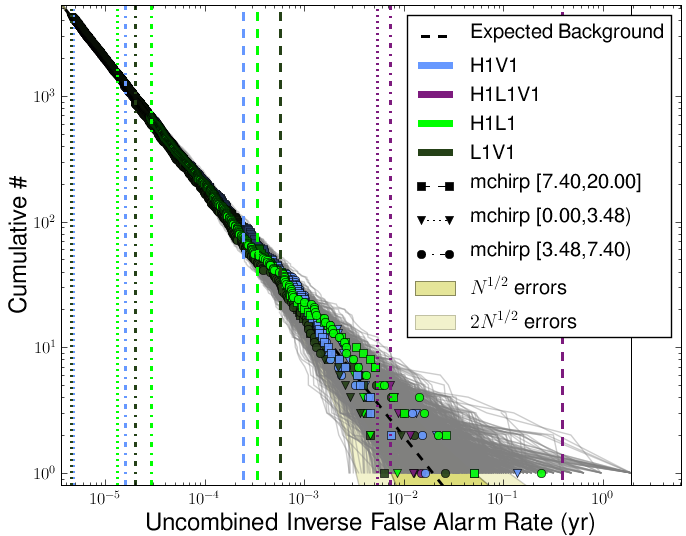
\includegraphics[width=4.5in]{figures/H1L1V1-ligolw_cbc_plotifar_FULL_DATA_CAT_4_VETO_cumhist_uncombined_ifar_ALL_DATA_PLOTTED_OPEN_BOX-931035296-4763191.png}}
\subfigure[Combined IFAR plot]{\label{fig:sample_plotifar_combined}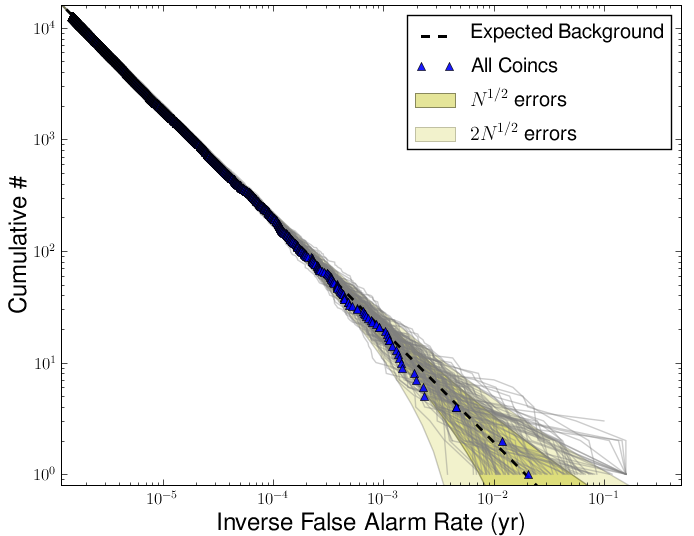
\includegraphics[width=4.5in]{figures/H1L1V1-ligolw_cbc_plotifar_FULL_DATA_CAT_4_VETO_cumhist_combined_ifar_ALL_DATA_PLOTTED_OPEN_BOX-931035296-4763191.png}}
\label{fig:sample_plotifar}
\caption{ Sample IFAR plots created by \texttt{ligolw\_cbc\_plotifar}. Both
plots taken from $\sim6$ weeks of \ac{S6} data, between GPS times 931035296 and
935798487.  In both plots, the black dashed-line indicates the expected
background distribution, yellow-shaded regions are the expected background $\pm
\sqrt{N}$ and $\pm \sqrt{2N}$, and gray lines are slide distributions when
treated as zero-lag. The blue triangles in the bottom plot indicate the
zero-lag distribution of combined IFARs. The top plot shows the uncombined IFAR
distribution, with each symbol representing a separate chirp-mass bin and each
color a coincident-detector combination. Colored dashed lines indicate maximum
(minimum) background \ac{FAR} (IFAR). See section \ref{sec:plotifar} for more
details.}
\end{figure}

\begin{figure}[p]
\label{fig:sample_plotcumhist}
\center
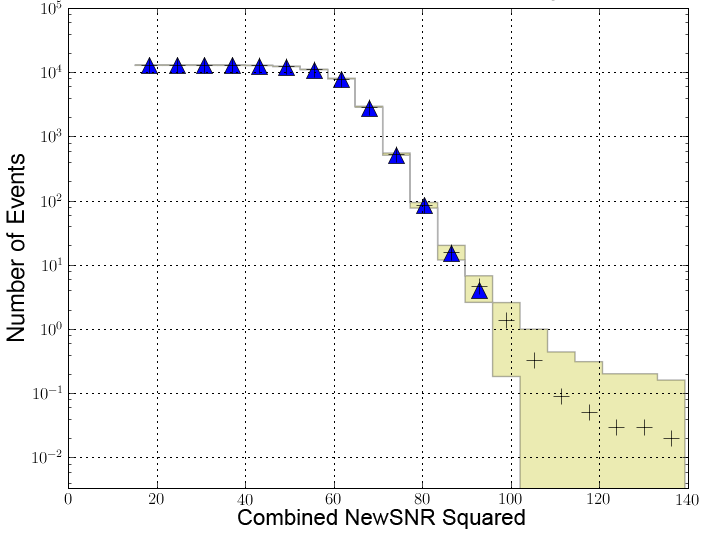
\includegraphics[width=5in]{figures/H1L1V1-ligolw_cbc_plotcumhist_FULL_DATA_CAT_4_VETO_cumhist_combined_snr_sq_ALL_DATA_PLOTTED_OPEN_BOX-931035296-4763191.png}
\caption{Sample cumulative histogram created by
\texttt{ligolw\_cbc\_plotcumhist}. Data taken from $\sim6$ weeks of S6 data,
between GPS times 931035296 and 935798487. The data is binned and the
cumulative number of triggers with New SNR greater-than or equal-to a given bin
are plotted on they y-axis. Zero-lag triggers are indicated by blue triangles.
The mean slide counts are indicated by the black crosses and the shaded regions
show the standard deviation across the slides. See section
\ref{sec:plotcumhist-plotslides} for more details.}
\end{figure}

\begin{figure}[p]
\center
\subfigure[Sample duration-per-slide plot for H1L1V1 time.]{\label{fig:sample_plotslide-H1L1V1_duration}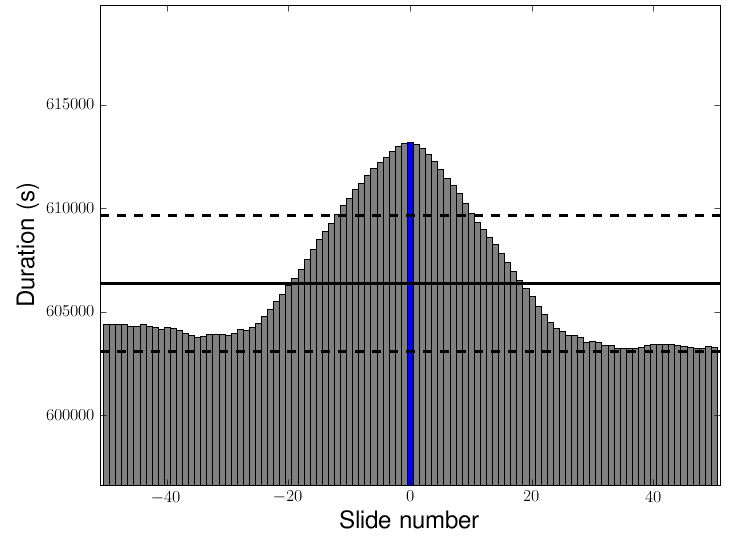
\includegraphics[width=4.5in]{figures/H1L1V1-ligolw_cbc_plotslides_FULL_DATA_CAT_4_VETO_durations_per_slide_ALL_DATA_PLOTTED-931035296-4763191.png}}
\subfigure[Sample duration-per-slide plot for H1L1 time.]{\label{fig:sample_plotslide-H1L1_duration}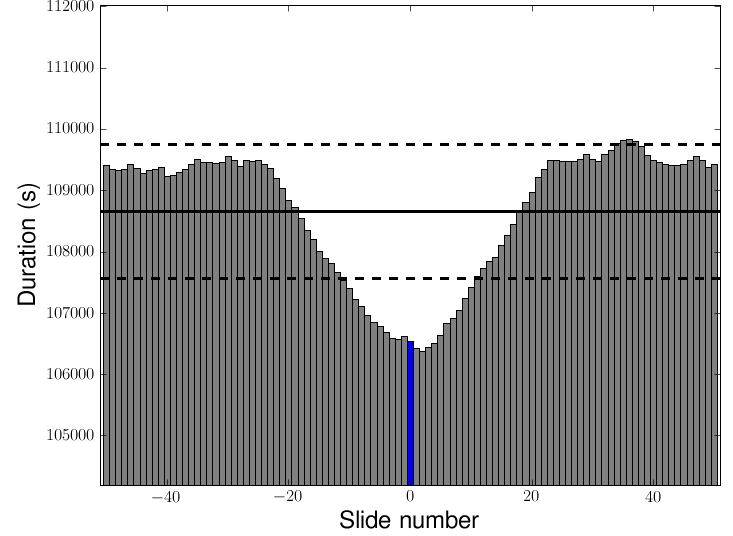
\includegraphics[width=4.5in]{figures/H1L1-ligolw_cbc_plotslides_FULL_DATA_CAT_4_VETO_durations_per_slide_ALL_DATA_PLOTTED-931035296-4763191.png}}
\label{fig:sample_plotslide-duration}
\caption{Sample duration-per-slide plots created by
\texttt{ligolw\_cbc\_plotslides}. Both plots taken from $\sim6$ weeks of S6
data, between GPS times 931035296 and 935798487. The top plots shows the
duration-per-slide for H1L1V1-coincident time; the bottom, H1L1-coincident
time. These plots are after CAT3 (cumulative) vetoes have been applied. Gray
bars show the duration in each slide; the blue bar shows the zero-lag duration.
The black solid line is the mean duration and the dashed lines show the
standard deviation. See section \ref{sec:plotcumhist-plotslides} for more
details.}
\end{figure}

\begin{figure}[p]
\label{fig:sample_plotslide-rate}
\center
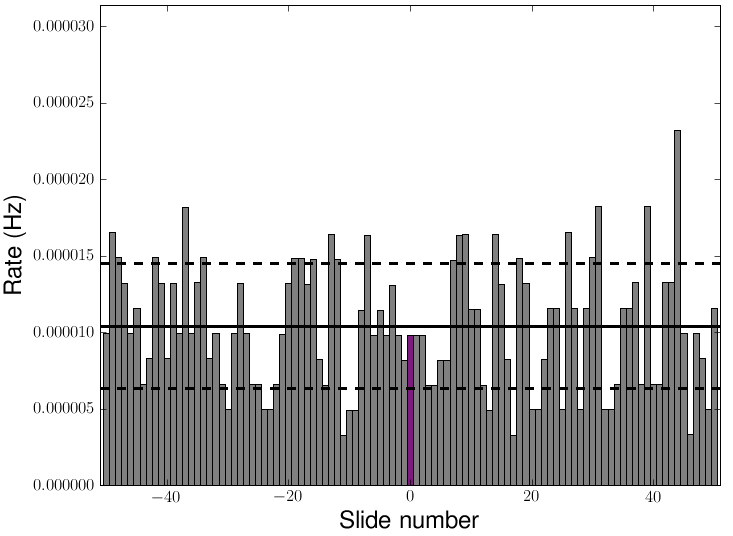
\includegraphics[width=5in]{figures/H1L1V1-ligolw_cbc_plotslides_FULL_DATA_CAT_4_VETO_H1L1V1_rates_ALL_DATA_PLOTTED_OPEN_BOX-931035296-4763191.png}
\caption{Sample trigger-rate-per-slide plot created by
\texttt{ligolw\_cbc\_plotslides}. The data is from the same time as Figure
\ref{fig:sample_plotslide-duration}. Shown is the rate of H1L1V1-coincident
triggers in H1L1V1-coincident time in each slide. Gray bars indicate the rate
in each slide; the purple bar shows the rate in zero-lag. (The color of the
zero-lag bar is based on the coincident \acp{IFO}.) The black solid line shows
the mean rate and the dashed lines the standard deviation.  See section
\ref{sec:plotcumhist-plotslides} for more details.}
\end{figure}

\begin{figure}[p]
\label{fig:plotfm-dist_v_mchirp}
\center
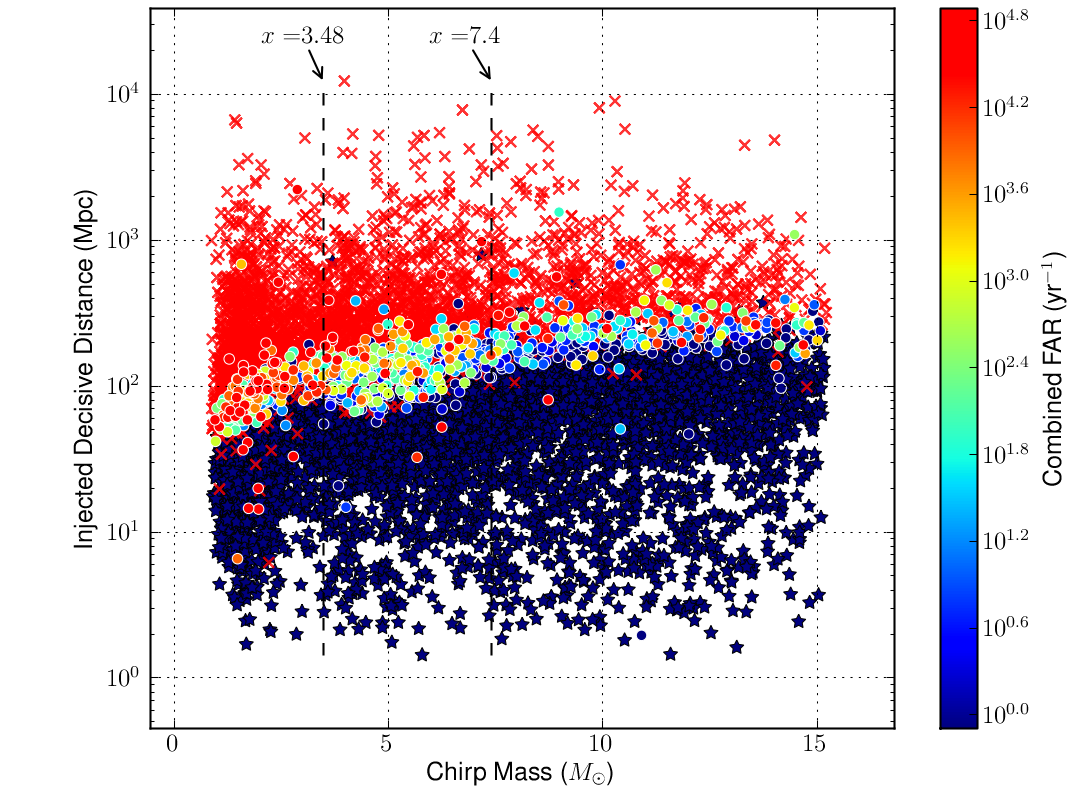
\includegraphics[width=6in]{figures/H1L1-ligolw_cbc_plotfm_fm_dist_v_param_ALLINJ_CAT_4_VETO_F1_ALLINJ_PLOTTED-956707143-4838544.png}
\caption{Sample decisive distance versus chirp mass plot for H1L1 time created
by \texttt{ligolw\_cbc\_plotfm}. The data is taken from $\sim6$ weeks of
\ac{S6} data, between GPS times 961545543 and 965174487. The blue stars are
injections found with a combined FAR equal to zero. The circles are
injections found with non-zero combined FAR; they are colored according to
their combined FAR. Missed injections are indicated by red crosses. The
black dashed lines show the chirp mass boundaries used. See section
\ref{sec:plotfm} for more details.}
\end{figure}

\begin{figure}[p]
\center
\subfigure[Chirp mass fractional difference versus end-time accuracy.]{\label{fig:plotfm-mchirp_frac_v_dt}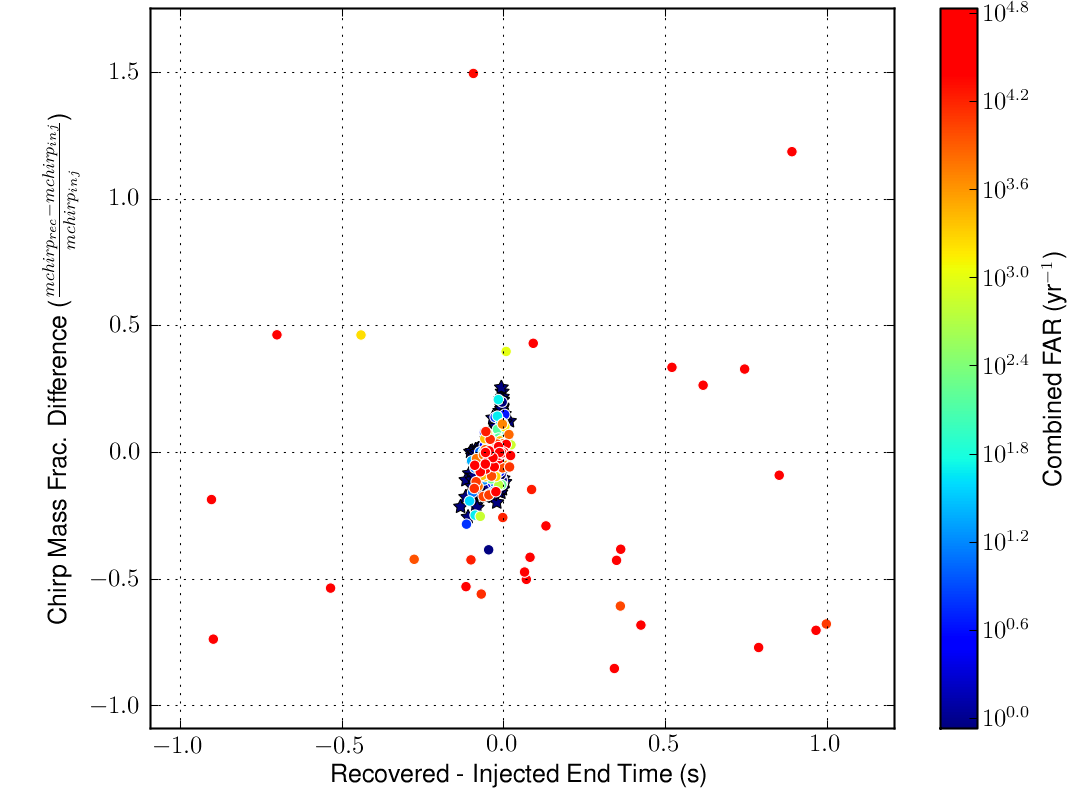
\includegraphics[width=4.5in]{figures/H1L1-ligolw_cbc_plotfm_fm_lin_plots_ALLINJ_CAT_4_VETO_F3_ALLINJ_PLOTTED-961545543-3628944.png}}
\subfigure[Injection type versus end-time accuracy.]{\label{fig:plotfm-injtag_v_dat}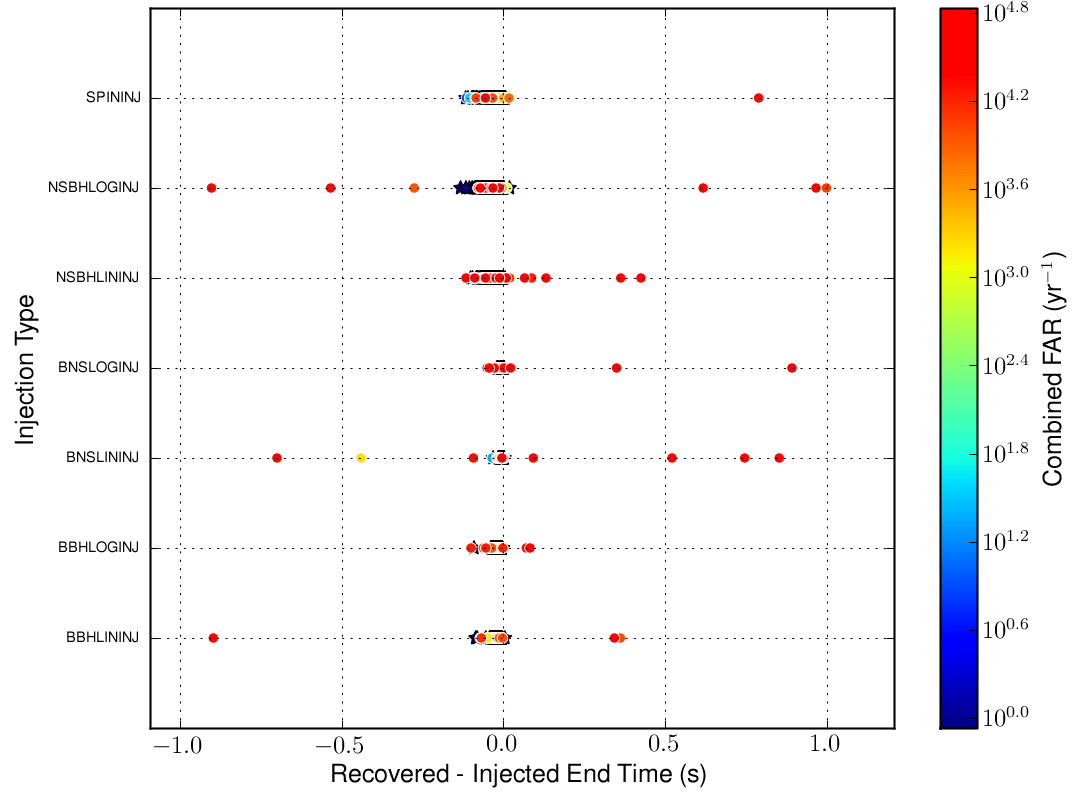
\includegraphics[width=4.5in]{figures/H1L1-ligolw_cbc_plotfm_fm_lin_plots_ALLINJ_CAT_4_VETO_F2_ALLINJ_PLOTTED-961545543-3628944.png}}
\caption{
More examples of \texttt{PlotFM} plots. The data used and color-coding is the
same as in Figure \ref{fig:plotfm-dist_v_mchirp}. Here, we have plotted the
fractional difference in recovered and injected chirp-mass (top) and the
injection type as a function of the difference in injected and recovered end
times. Plots such as these help to establish what ``found" injections are
actually due to noise triggers occuring within the injection-finding
time-window, $t_{\mathrm{injfind}}$, of an injection. (See section
\ref{sec:Pipedown-injBranch}.) For example, the orange-red dots (representing
``found" injections with high combined FAR) that are scattered across the
fractional chirp-mass and end-time recovery are most likely due to noise
triggers occuring with $\pm t_{\mathrm{injfind}}$ of an injection and not due
to the injection itself. Contrast these to the blue stars --- injections
``found" with 0 combined FAR --- which all have good recovered parameters. It
is therefore highly likely that these triggers came from injections.}
\label{fig:plotfm-example_v_dt}
\end{figure}

\clearpage

\begin{figure}[p]
\label{fig:example-loudest_all_data_events}
\center
\fbox{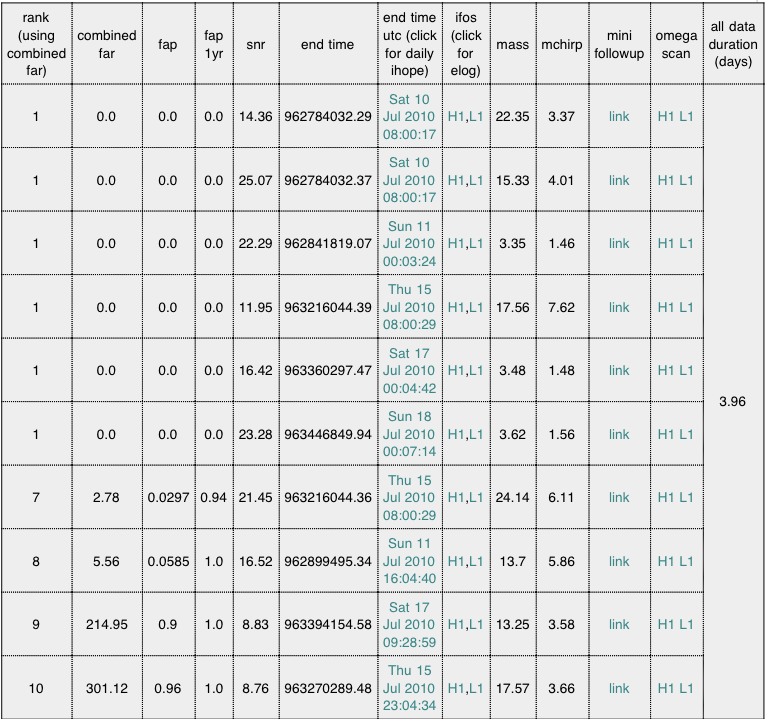
\includegraphics[width=6in]{figures/all_data-loudest_events/example-loudest_all_data_events.png}}
\caption{An example \texttt{all\_data} loudest-events list created by
\texttt{PrintLC} when run in Pipedown. This list shows the top ten loudest
(i.e., most signficant) events, as ranked by combined FAR, in a search. The
``end time utc" column provides a link to the daily \ihope~page
\cite{Pekowsky:thesis}, the ``ifos" column provides a link to the e-log page,
the ``mini followup" column provides a link to the MiniFollowup page, and the
``omega scan" column provides a link to the Omega scans of the event. These
links are used to investigate what caused each event. See section
\ref{sec:printlc-minifups} for more details.}
\end{figure}

\begin{figure}[p]
\center
\subfigure[A screen shot of the MiniFollowup page.]{\label{fig:sample-minifup_hardware_inj-screenshot}\fbox{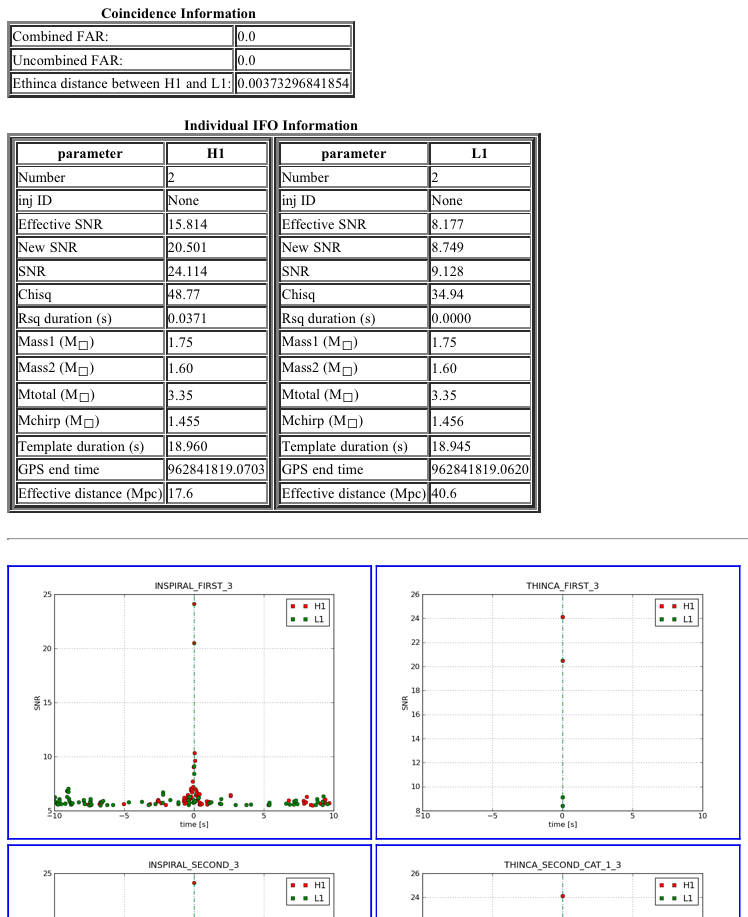
\includegraphics[height=3.5in]{figures/all_data-loudest_events/minifup-example_page.png}}}
\subfigure[A close-up of the \texttt{INSPIRAL\_FIRST} MiniFollowup plot.]{\label{fig:sample-minifup_hardware_inj-inspiral_first}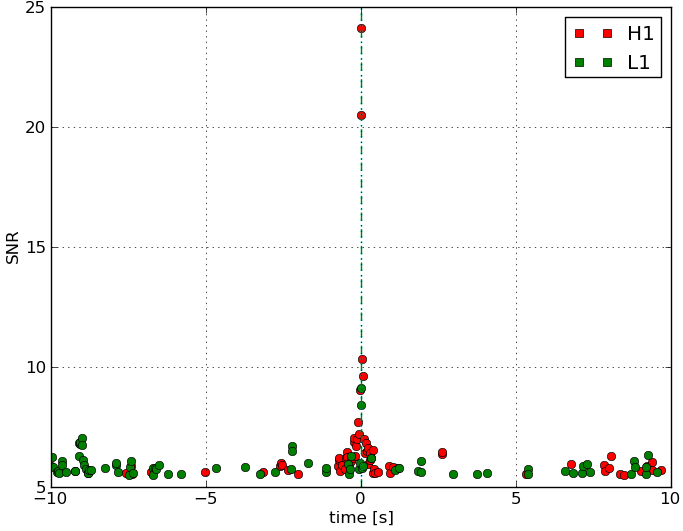
\includegraphics[width=4.25in]{figures/all_data-loudest_events/H1L1-FULL_DATA_CAT_2_VETO_FULL_DATA_map-INSPIRAL_FIRST-3_LOUDEST_ALL_DATA_EVENTS_BY_COMBINED_FAR_SUMMARY-962755143-1209744.png}}
\label{fig:sample-minifup_hardware_inj}
\caption{The MiniFollowup page for the third event, a hardware injection, in
the loudest events list shown in Figure
\ref{fig:example-loudest_all_data_events}. The top figure shows a screen shot
of the page. On this page, there is a table giving more details about the
single-detector parameters, as well as plots of SNR versus time within $\pm
10\,$s of the event are shown for each stage in the \hipe~pipeline (first
inspiral --- second coincidence). The bottom figure shows
\texttt{INSPIRAL\_FIRST} SNR verus time plot from the page. We see that there
is a spike in SNR at the time of the injection in both detectors surrounded by
relatively low-level noise. This is what we would expect to see for a \ac{GW}
signal.}
\end{figure}

\begin{figure}[p]
\center
\subfigure[The H1 Omega scan.]{\label{fig:sample-omega_hardware_inj-H1}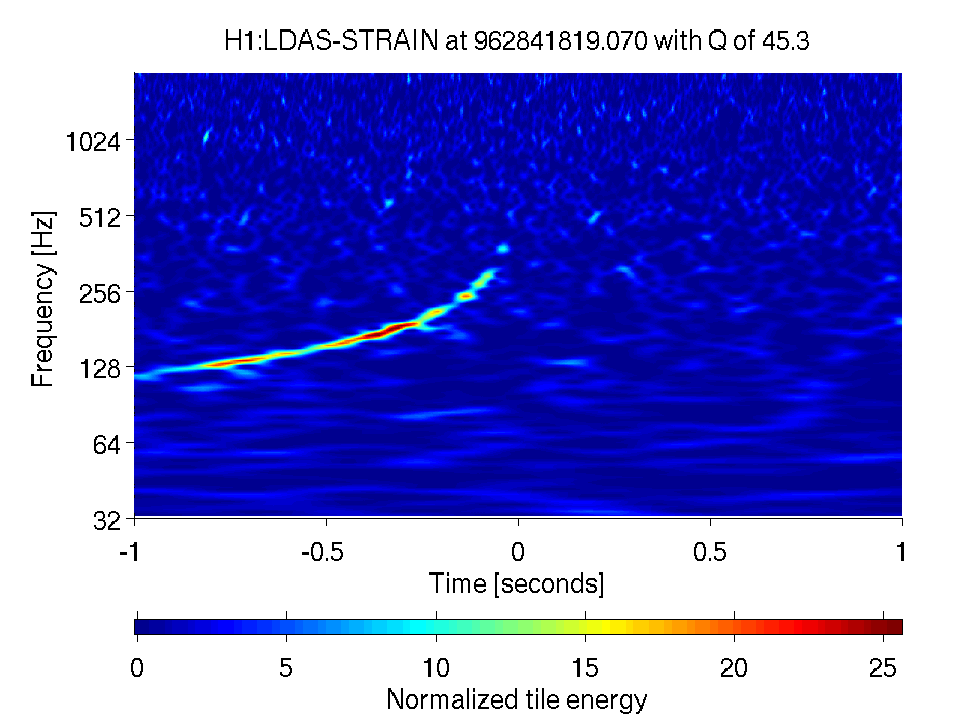
\includegraphics[height=3in]{figures/all_data-loudest_events/962841819_0703125_H1_LDAS-STRAIN_2_00_spectrogram_whitened.png}}
\subfigure[The L1 Omega scan.]{\label{fig:sample-omega_hardware_inj-L1}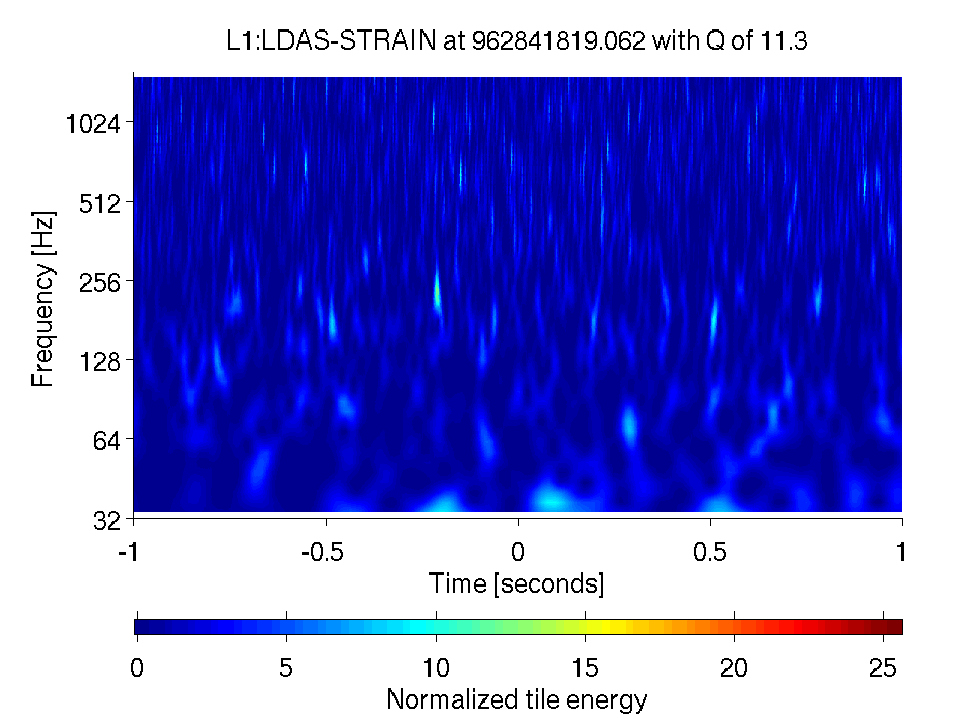
\includegraphics[height=3in]{figures/all_data-loudest_events/962841819_062011718_L1_LDAS-STRAIN_2_00_spectrogram_whitened.png}}
\label{fig:sample-omega_hardware_inj}
\caption{An example of an Omega scan. These scans are of the hardware injection
shown in Figure \ref{fig:sample-minifup_hardware_inj}. The ``normalized tile
energy'' is roughly equivalent to SNR$^2$/2 in a time-frequency tile. For
Gaussian noise in the absence of signal, the normalized tile energy rarely
exceeds 8. In the H1 scan (top) a chirp pattern is clearly visible (compare
this to Figure \ref{fig:GW_evolution-freq}). However, in the L1 scan (bottom)
nothing can be seen, since the injection had a SNR $<\sim10$ in L1. This is
why we do not simply look at Omega scans to determine if an event is a GW
signal. Scans can provide clues as to the cause of an event. In this case, due
to the clear chirp and the lack of noticeable noise in L1 (c.f. Figure
\ref{fig:sample-omega_slide}), we can be confident this is a GW signal. See section
\ref{sec:printlc-minifups} for more details.}
\end{figure}

\begin{figure}[p]
\label{fig:example-loudest_slide_events}
\center
\fbox{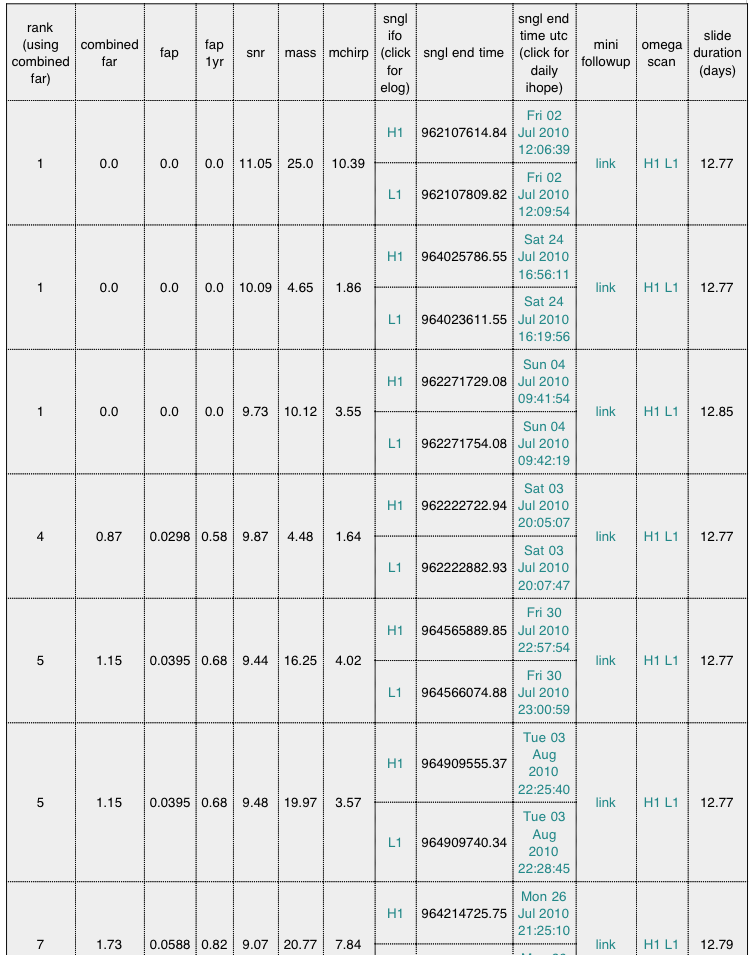
\includegraphics[width=6in]{figures/slide-loudest_events/example-loudest_slide_events.png}}
\caption{An example \texttt{slide} loudest-events list created by
\texttt{PrintLC} when run in Pipedown. This is similar to the \texttt{all-data}
loudest-events list shown in Figure \ref{fig:example-loudest_all_data_events},
except that the un-slid single-detector end times are shown. This allows us to
easily followup loud slide events which --- since they determine the \ac{FAR}
of potential signals --- are the events that have the greatest impact on the
pipeline to detect. We can use this information to provide clues for new
vetoes. See Chapter \ref{ch:s6_results} for how these \emph{loudest-slide
studies} were carried out in S6.}
\end{figure}

\begin{figure}[p]
\center
\label{fig:sample-minifup_slide}
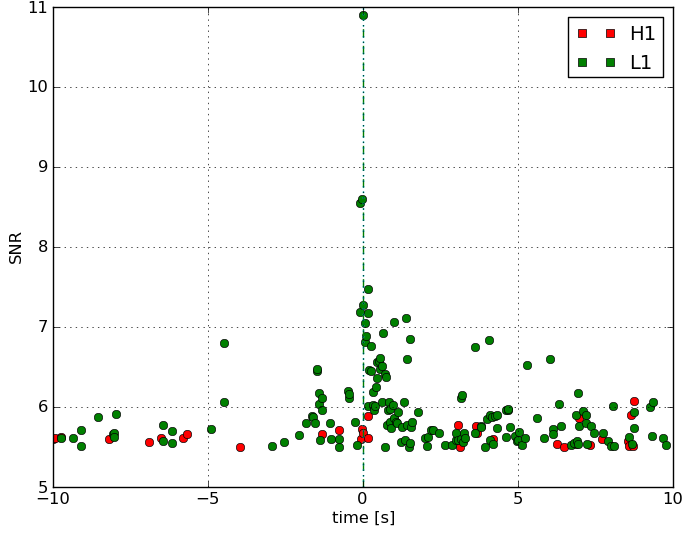
\includegraphics[width=4.8in]{figures/slide-loudest_events/H1L1-FULL_DATA_CAT_3_VETO_FULL_DATA_map-INSPIRAL_FIRST-3_LOUDEST_SLIDE_EVENTS_BY_COMBINED_FAR_SUMMARY-961545543-3628944.png}
\caption{The \texttt{INSPIRAL\_FIRST} MiniFollowup plot for the first loudest
slide event (the one on Friday July 2 2010) shown in Figure
\ref{fig:example-loudest_slide_events}. Contrast this to the MiniFollowup plot
shown in Figure \ref{fig:sample-minifup_hardware_inj-inspiral_first}, which is
of a hardware injection. In this case, the SNR of triggers is elevated in L1
around the time of the event, suggesting that an environmental or instrumental
source has caused heightened noise in L1 at that time.}
\end{figure}

\begin{figure}[p]
\center
\subfigure[The H1 Omega scan.]{\label{fig:sample-omega_slide-H1}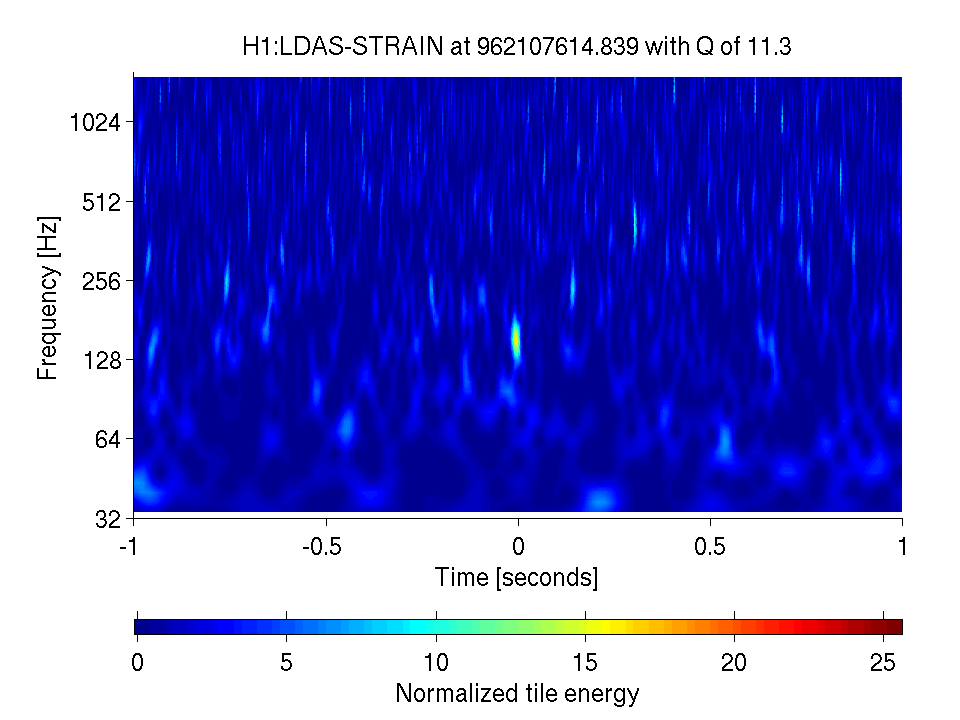
\includegraphics[height=3in]{figures/slide-loudest_events/962107614_839111328_H1_LDAS-STRAIN_2_00_spectrogram_whitened.png}}
\subfigure[The L1 Omega scan.]{\label{fig:sample-omega_slide-L1}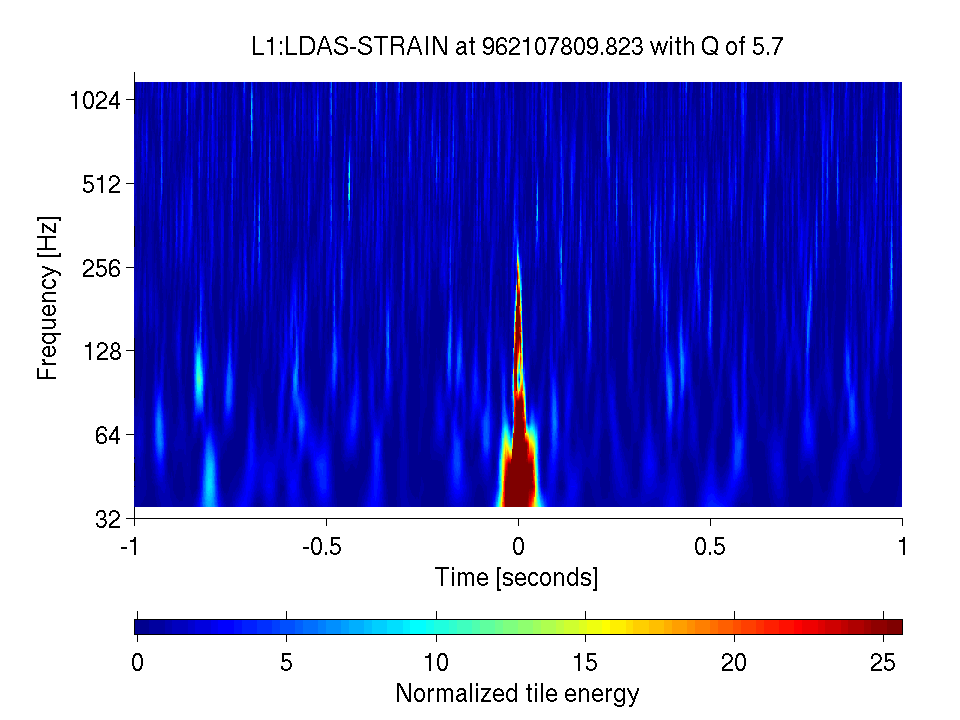
\includegraphics[height=3in]{figures/slide-loudest_events/962107809_823242187_L1_LDAS-STRAIN_2_00_spectrogram_whitened.png}}
\label{fig:sample-omega_slide}
\caption{The Omega scans of the slide event shown in Figure
\ref{fig:sample-minifup_slide}. Compare these scans to those of the hardware
injection in Figure \ref{fig:sample-omega_hardware_inj}. The H1 scan is
relatively clean, and so it could contain a GW signal. The L1 scan, however,
clearly shows a low-frequency glitch; this looks nothing like a chirp we would
expect to see from a GW. Based on this, we can search the e-log and use other
tools (some of which are discussed in Chapter \ref{ch:s6_results}) to
understand what caused this glitch in L1. If an environmental cause can be
found, we can veto this period of time in L1, which would remove this slide
coincidence from the background estimation.} 
\end{figure}

\begin{figure}[p]
\label{fig:sample-daily_ihope-slide}
\center
\fbox{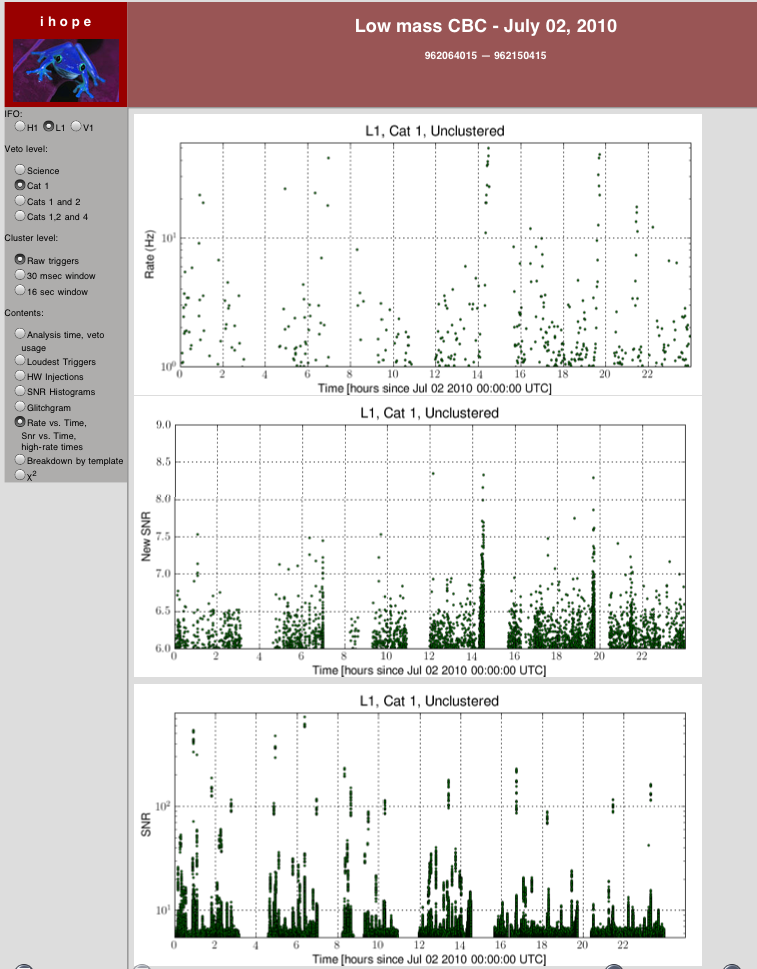
\includegraphics[height=7in]{figures/slide-loudest_events/example-daily_ihope_slide.png}}
\caption{A screen shot of a daily \ihope~page. This page is from the same day
as the loudest slide event shown in Figures \ref{fig:sample-minifup_slide} and
\ref{fig:sample-omega_slide}. It can be accessed from the loudest-events table
by clicking on the \texttt{sngl end time utc} column for the trigger. Shown is the
rate, New \ac{SNR} and \ac{SNR} of triggers as a function of time for L1 after
CAT1 vetoes have been applied. As evident from the side bar, there are several
other plots and lists available for all the detectors at various vetoes and
clustering windows. For more details on daily \ihope~see \cite{Pekowsky:thesis}.}
\end{figure}

\begin{figure}[p]
\label{fig:sample-elog-slide}
\center
\fbox{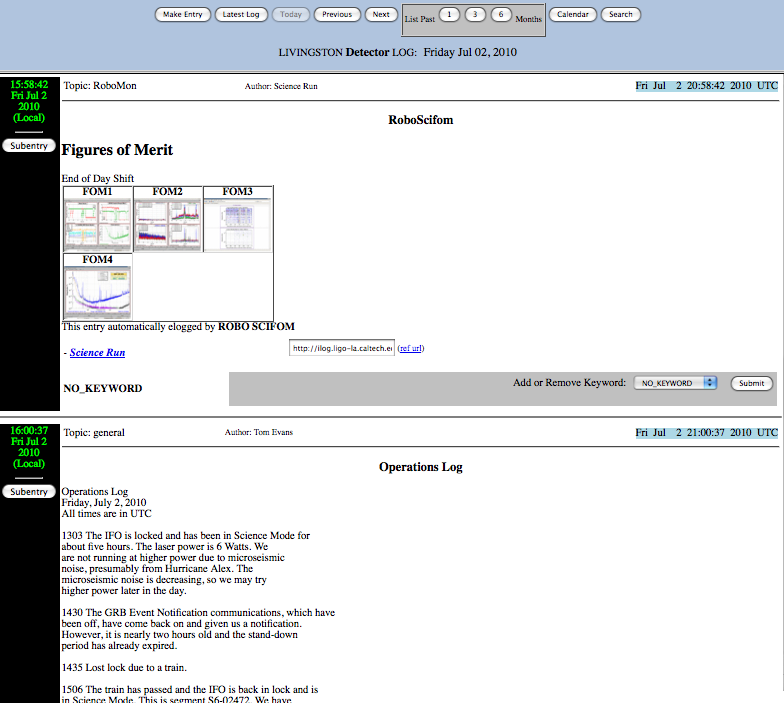
\includegraphics[width=6in]{figures/slide-loudest_events/sample-elog.png}}
\caption{A screen shot of a L1 e-log. The day shown is from the same day as the
loudest slide event shown in Figures \ref{fig:sample-minifup_slide} and
\ref{fig:sample-omega_slide}. It can be accessed from the loudest-events table
by clicking on the ``L1" in the \texttt{sngl ifo} column for the trigger. For a
further disucssion of the e-log page see section \ref{sec:printlc-minifups}.}
\end{figure}

\begin{figure}[p]
\center
\subfigure[All injections.]{\label{fig:sample-printmissed_ALLINJ}\fbox{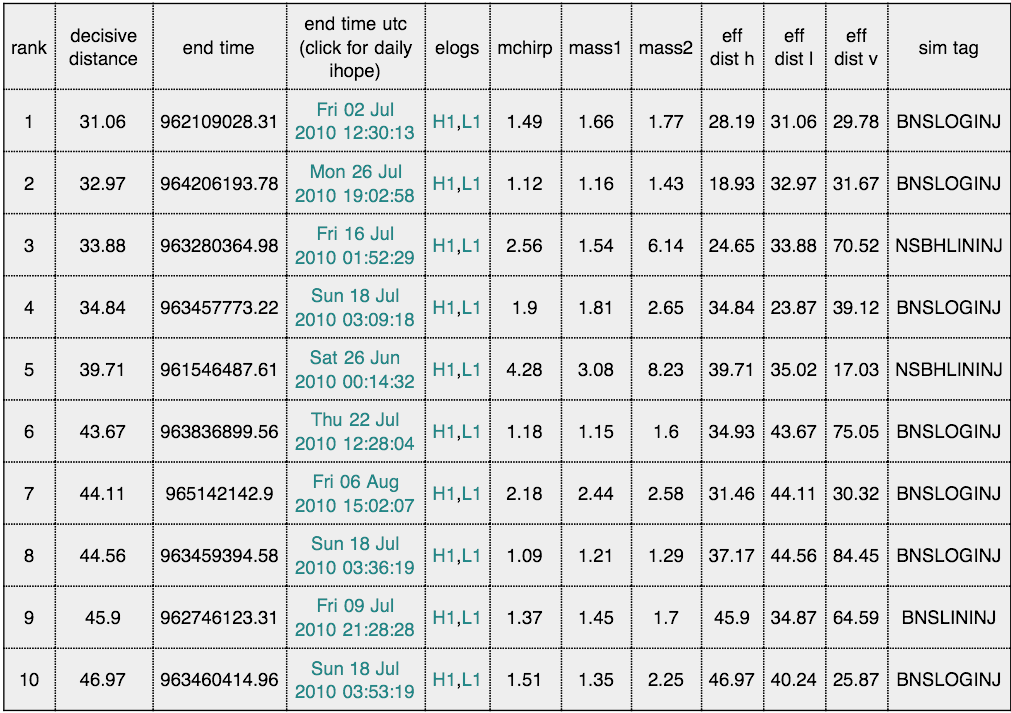
\includegraphics[width=6in]{figures/missed_injection-example/example-printmissed_ALLINJ.png}}}
\subfigure[The \texttt{BNSLOGINJ} table.]{\label{fig:sample-printmissed_BNSLOGINJ}\fbox{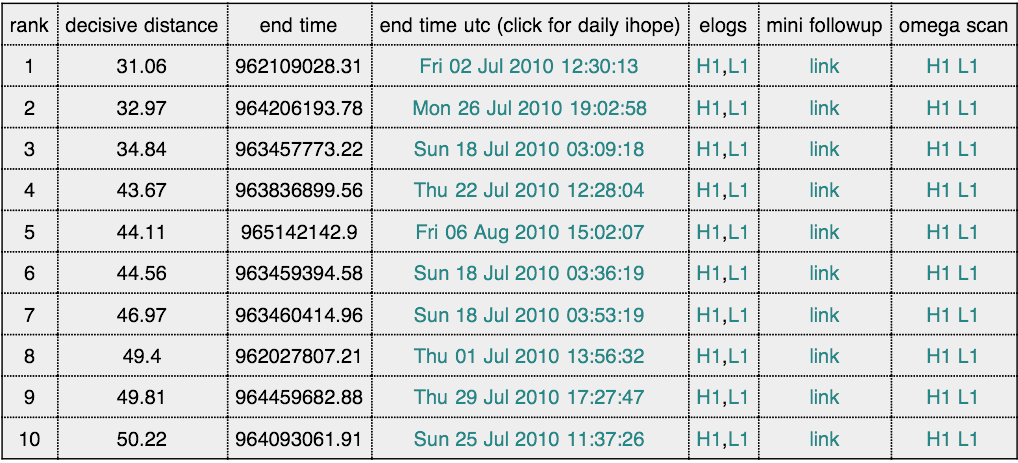
\includegraphics[width=6in]{figures/missed_injection-example/example-printmissed_BNSLOGINJ.png}}}
\label{fig:sample-printmissed}
\caption{Example tables produced by \texttt{PrintMissed} when run in Pipedown.
The top table shows the 10 closest missed injections out of all of the
injection runs. The bottom table shows the 10 closest missed injections in the
\texttt{BNSLOGINJ} run. Note that in the second table, MiniFollowup and Omega
scan links have been added. See section \ref{sec:printmissed-printsims} for
more information.}
\end{figure}

\begin{figure}[p]
\center
\subfigure[A screen shot of the found/missed table produced by \texttt{MiniFollowups}.]{\label{fig:sample-minifup_missedinj-table}\fbox{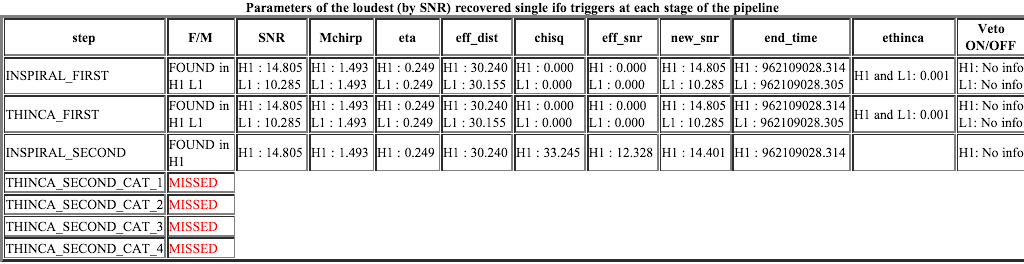
\includegraphics[width=6in]{figures/missed_injection-example/example-missedinj_minifup.png}}}
\subfigure[The \texttt{INSPIRAL\_FIRST} plot from the mini-followup page for this missed injection.]{\label{fig:sample-minifup_missedinj-plot}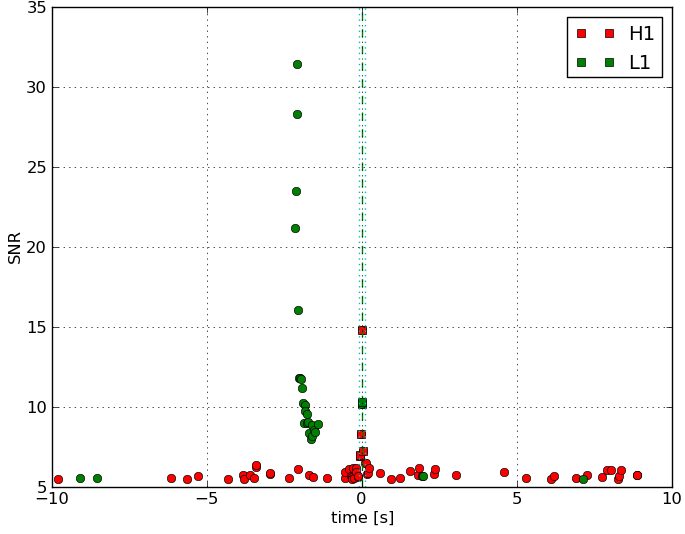
\includegraphics[width=5in]{figures/missed_injection-example/H1L1-BNSLOGINJ_CAT_4_VETO_BNSLOGINJ_map-INSPIRAL_FIRST-1_CLOSEST_MISSED_INJECTIONS_SUMMARY-961545543-3628944.png}}
\label{fig:sample-minifup_missedinj}
\caption{An example of the output produced by \texttt{MiniFollowups} when run
on a missed injection. The top figure is a screen shot of the found/missed
table that traces whether or not the injection was found, and with what
parameters, at each stage in the pipeline. The bottom figure shows the
\texttt{INSPIRAL\_FIRST} plot created for the event. As with the MiniFollowup
plots shown in Figure \ref{fig:sample-minifup_hardware_inj-inspiral_first},
this plot shows the SNR versus time of single-detector triggers within $\pm
10\,$s of the injection. Here, a large spike in SNR is evident in L1 just prior
to the injection. This followup is for the closest missed injection shown in
the tables shown in Figure \ref{fig:sample-printmissed}.}
\end{figure}

\begin{figure}[p]
\center
\subfigure[The H1 Omega scan.]{\label{fig:sample-omega_missedinj-H1}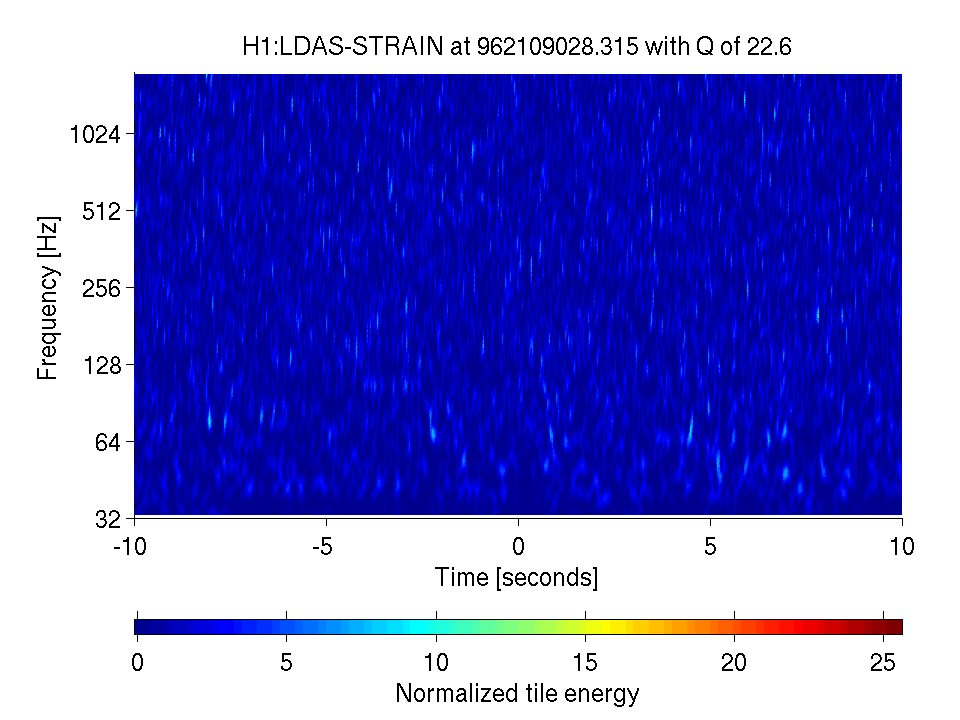
\includegraphics[width=4.25in]{figures/missed_injection-example/962109028_314747572_H1_LDAS-STRAIN_20_00_spectrogram_whitened.png}}
\subfigure[The L1 Omega scan.]{\label{fig:sample-omega_missedinj-L1}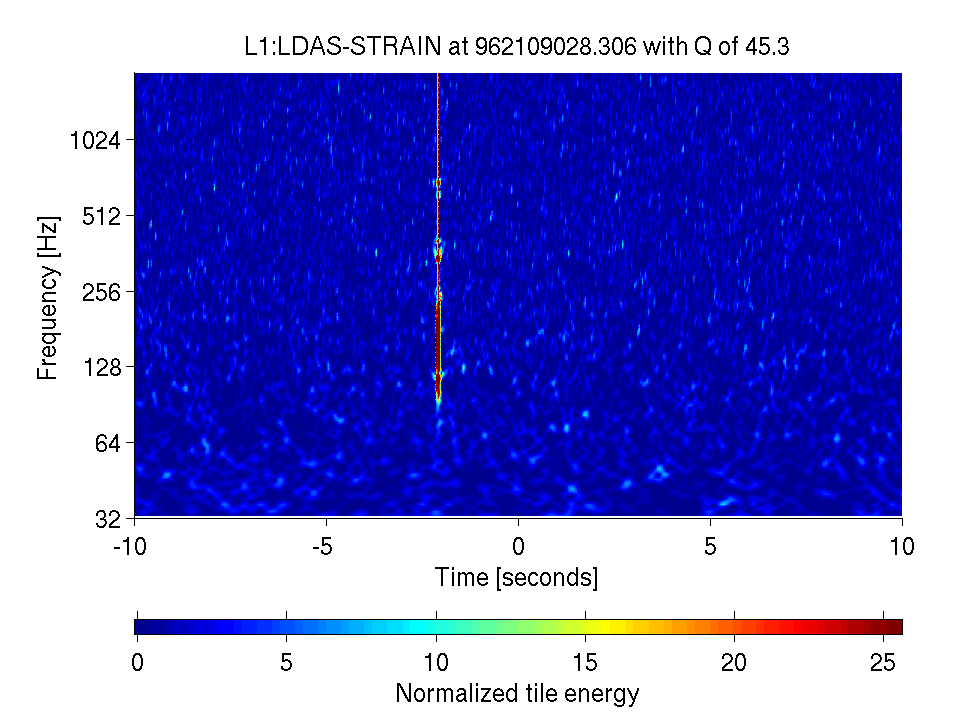
\includegraphics[width=4.25in]{figures/missed_injection-example/962109028_306081057_L1_LDAS-STRAIN_20_00_spectrogram_whitened.png}}
\label{fig:sample-omega_missedinj}
\caption{The Omega scans of the missed \texttt{BNSLOGINJ} injection detailed in
Figure \ref{fig:sample-minifup_missedinj}. The H1 scan is clean, but the L1
scan shows a short-duration broadband glitch $\sim2\,$s before the injection's
end time (which is placed at $0\,$s on the spectrograms). The presence of this
glitch is most likely reason why the injection was missed. Note that the H1
(and possibly the L1) \ac{SNR} of the injection is large enough to be seen in
Omega scan. Nothing is seen because Omega scans do not currenlty show software
injections.}
\end{figure}

\begin{figure}[p]
\center
\subfigure[All injections.]{\label{fig:sample-printsims_ALLINJ}\fbox{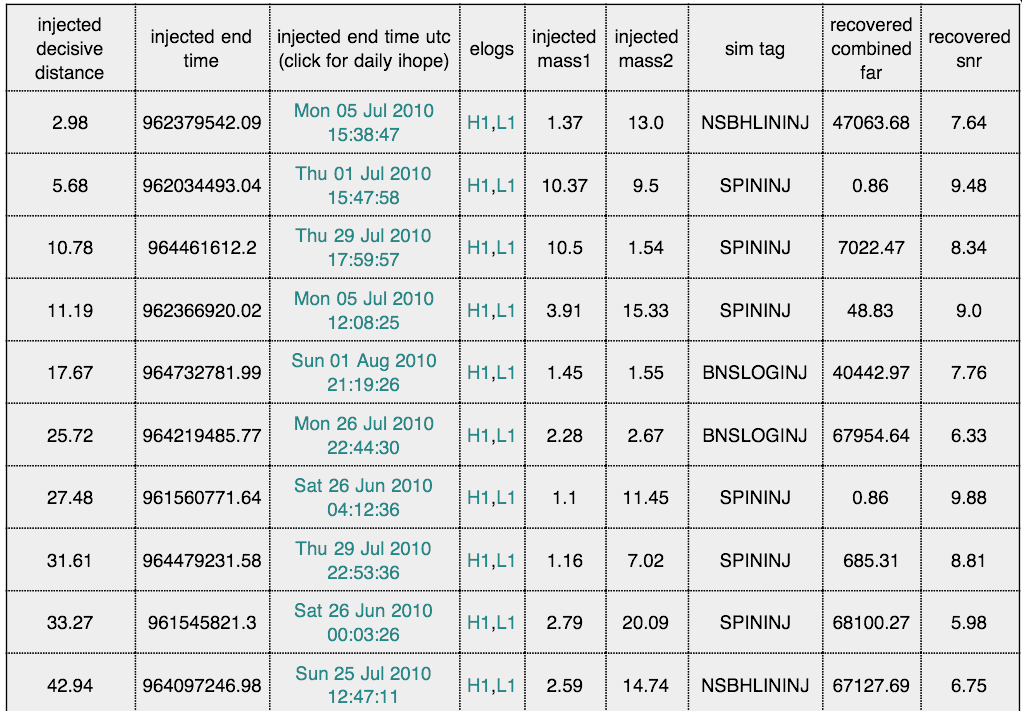
\includegraphics[width=5in]{figures/example-printsims_ALLINJ.png}}}
\subfigure[The \texttt{BNSLOGINJ} table.]{\label{fig:sample-printsims_BNSLOGINJ}\fbox{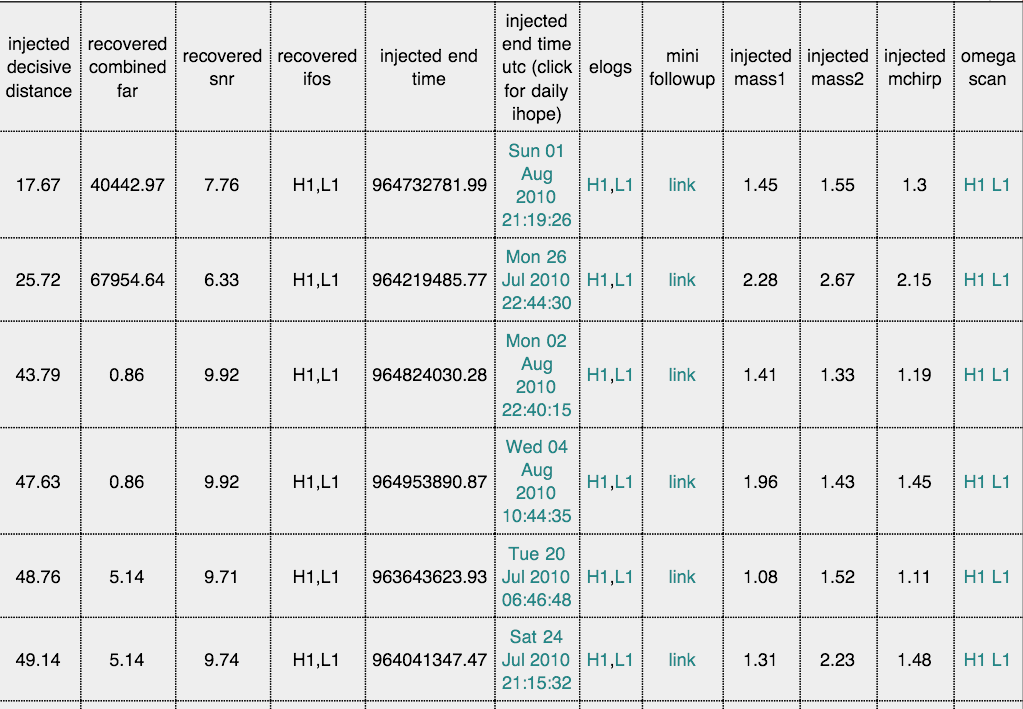
\includegraphics[width=5in]{figures/example-printsims_BNSLOGINJ.png}}}
\label{fig:sample-printsims}
\caption{An example of the tables produced by \texttt{PrintSims} when run in
Pipedown. The top table shows a portion of the quiestest found table for all
the injection runs. The bottom table shows a portion of \texttt{BNSLOGINJ}
table. Note that in the latter table, MiniFollowup and Omega scan links have
been added. See section \ref{sec:printmissed-printsims} for more details.}
\end{figure}

\begin{figure}
\label{fig:sample_ihope_page}
\begin{center}
\fbox{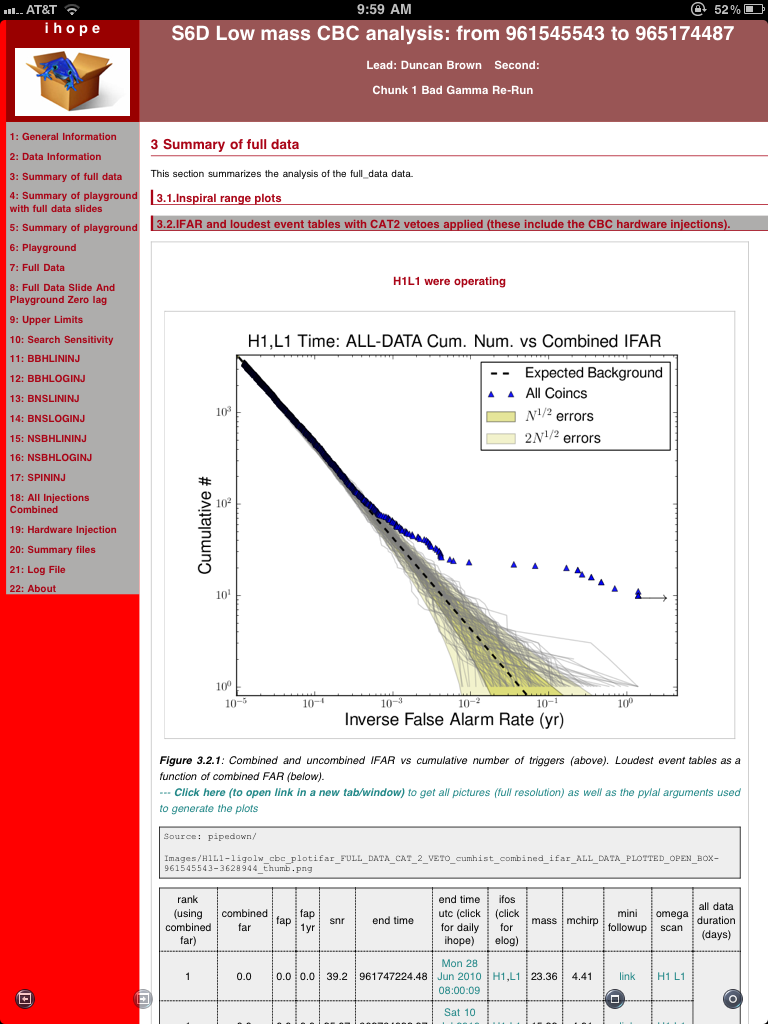
\includegraphics[height=7in]{figures/IhopePage-example.png}}
\end{center}
\caption{A screen shot of an \ihope~page. This is the final page that is
created after \ihope~has completed. It summarizes all of the data and plots
generated by \ihope~and provides links to auxillary pages to further followup
triggers. For more details, see section \ref{sec:ihope_page}.}
\end{figure}
